% ******************************* PhD Thesis Template **************************
% Please have a look at the README.md file for info on how to use the template

\documentclass[a4paper,12pt,times,numbered,print,index]{Classes/PhDThesisPSnPDF}

% ******************************************************************************
% ******************************* Class Options ********************************
% *********************** See README for more details **************************
% ******************************************************************************

% `a4paper'(The University of Cambridge PhD thesis guidelines recommends a page
% size a4 - default option) or `a5paper': A5 Paper size is also allowed as per
% the Cambridge University Engineering Deparment guidelines for PhD thesis
%
% `11pt' or `12pt'(default): Font Size 10pt is NOT recommended by the University
% guidelines
%
% `oneside' or `twoside'(default): Printing double side (twoside) or single
% side.
%
% `print': Use `print' for print version with appropriate margins and page
% layout. Leaving the options field blank will activate Online version.
%
% `index': For index at the end of the thesis
%
% `draftclassic': For draft mode without loading any images (same as draft in book)
%
% `draft': Special draft mode with line numbers, images, and water mark with
% timestamp and custom text. Position of the text can also be modified.
%
% `abstract': To generate only the title page and abstract page with
% dissertation title and name, to submit to the Student Registry
%
% `chapter`: This option enables only the specified chapter and it's references
%  Useful for review and corrections.
%
% ************************* Custom Page Margins ********************************
%
% `custommargin`: Use `custommargin' in options to activate custom page margins,
% which can be defined in the preamble.tex. Custom margin will override
% print/online margin setup.
%
% *********************** Choosing the Fonts in Class Options ******************
%
% `times' : Times font with math support. (The Cambridge University guidelines
% recommend using times)
%
% `fourier': Utopia Font with Fourier Math font (Font has to be installed)
%            It's a free font.
%
% `customfont': Use `customfont' option in the document class and load the
% package in the preamble.tex
%
% default or leave empty: `Latin Modern' font will be loaded.
%
% ********************** Choosing the Bibliography style ***********************
%
% `authoryear': For author-year citation eg., Krishna (2013)
%
% `numbered': (Default Option) For numbered and sorted citation e.g., [1,5,2]
%
% `custombib': Define your own bibliography style in the `preamble.tex' file.
%              `\RequirePackage[square, sort, numbers, authoryear]{natbib}'.
%              This can be also used to load biblatex instead of natbib
%              (See Preamble)
%
% **************************** Choosing the Page Style *************************
%
% `default (leave empty)': For Page Numbers in Header (Left Even, Right Odd) and
% Chapter Name in Header (Right Even) and Section Name (Left Odd). Blank Footer.
%
% `PageStyleI': Chapter Name next & Page Number on Even Side (Left Even).
% Section Name & Page Number in Header on Odd Side (Right Odd). Footer is empty.
%
% `PageStyleII': Chapter Name on Even Side (Left Even) in Header. Section Number
% and Section Name in Header on Odd Side (Right Odd). Page numbering in footer

\usepackage{algorithm}
\usepackage{algorithmic}
\usepackage{graphicx}
\usepackage{url}
\usepackage{color}
\usepackage{flushend}

\newtheorem{theorem}{Theorem}[section]
\newtheorem{lemma}[theorem]{Lemma}
\newtheorem{hypothesis}[theorem]{$\mathcal{H}$}
\newtheorem{proposition}[theorem]{Proposition}
\newtheorem{corollary}[theorem]{Corollary}

\newenvironment{proof}[1][Proof]{\begin{trivlist}
\item[\hskip \labelsep {\bfseries #1}]}{\end{trivlist}}
\newenvironment{definition}[1][Definition]{\begin{trivlist}
\item[\hskip \labelsep {\bfseries #1}]}{\end{trivlist}}
\newenvironment{example}[1][Example]{\begin{trivlist}
\item[\hskip \labelsep {\bfseries #1}]}{\end{trivlist}}
\newenvironment{remark}[1][Remark]{\begin{trivlist}
\item[\hskip \labelsep {\bfseries #1}]}{\end{trivlist}}

% tombstones for the end of proof
\newcommand{\qed}{\nobreak \ifvmode \relax \else
      \ifdim\lastskip<1.5em \hskip-\lastskip
      \hskip1.5em plus0em minus0.5em \fi \nobreak
      \vrule height0.75em width0.5em depth0.25em\fi}

\newcommand\hyptref[1]{$\mathcal{H}$[\ref{#1}]}
\newcommand\propref[1]{$\mathcal{P}$[\ref{#1}]}
\newcommand\prop[1]{(\mathcal{P}_{#1})}




% ********************************** Preamble **********************************
% Preamble: Contains packages and user-defined commands and settings
% ******************************************************************************
% ****************************** Custom Margin *********************************

% Add `custommargin' in the document class options to use this section
% Set {innerside margin / outerside margin / topmargin / bottom margin}  and
% other page dimensions
\ifsetCustomMargin
  \RequirePackage[left=37mm,right=30mm,top=35mm,bottom=30mm]{geometry}
  \setFancyHdr % To apply fancy header after geometry package is loaded
\fi

% ******************************************************************************
% ****************************** Allow space at bottom of page *********************************
\raggedbottom

% *****************************************************************************
% ******************* Fonts (like different typewriter fonts etc.)*************

% Add `customfont' in the document class option to use this section

\ifsetCustomFont
  % Set your custom font here and use `customfont' in options. Leave empty to
  % load computer modern font (default LaTeX font).
  %\RequirePackage{helvet}

  % For use with XeLaTeX
  %  \setmainfont[
  %    Path              = ./libertine/opentype/,
  %    Extension         = .otf,
  %    UprightFont = LinLibertine_R,
  %    BoldFont = LinLibertine_RZ, % Linux Libertine O Regular Semibold
  %    ItalicFont = LinLibertine_RI,
  %    BoldItalicFont = LinLibertine_RZI, % Linux Libertine O Regular Semibold Italic
  %  ]
  %  {libertine}
  %  % load font from system font
  %  \newfontfamily\libertinesystemfont{Linux Libertine O}
\fi

% *****************************************************************************
% **************************** Custom Packages ********************************

% ************************* Algorithms and Pseudocode **************************

\usepackage{amsmath}
\usepackage{empheq}
\usepackage{amssymb}
\usepackage{algorithm}
\usepackage{algpseudocode}
\usepackage{graphicx}
\usepackage{float}
\usepackage{placeins}
%\usepackage{url}
\usepackage{color}
\usepackage{flushend}
\usepackage{overpic}
\usepackage[table]{xcolor}
\usepackage{multirow}
%\usepackage{ulem}
\usepackage{natbib}
\usepackage{bibentry}
\nobibliography*

\usepackage{pgfplots}
\usepackage[utf8]{inputenc}

\usepackage{tikz}
\usetikzlibrary{shapes.geometric, arrows}

\pgfplotsset{compat=1.9}

%\usepgfplotslibrary{external}
%\tikzexternalize

%\usepackage[colorlinks = true,
            %linkcolor = blue,
            %urlcolor  = blue,
            %citecolor = blue,
            %anchorcolor = blue]{hyperref}
%\newcommand{\colorhref}[3][blue]{\href{#2}{\color{#1}{#3}}}%
\usepackage{hyperref}
% ********************Captions and Hyperreferencing / URL **********************

% Captions: This makes captions of figures use a boldfaced small font.
%\RequirePackage[small,bf]{caption}

\RequirePackage[labelsep=space,tableposition=top]{caption}
\renewcommand{\figurename}{Fig.} %to support older versions of captions.sty


% *************************** Graphics and figures *****************************

%\usepackage{rotating}
%\usepackage{wrapfig}

% Uncomment the following two lines to force Latex to place the figure.
% Use [H] when including graphics. Note 'H' instead of 'h'
%\usepackage{float}
%\restylefloat{figure}

% Subcaption package is also available in the sty folder you can use that by
% uncommenting the following line
% This is for people stuck with older versions of texlive
%\usepackage{sty/caption/subcaption}
\usepackage{subcaption}

% ********************************** Tables ************************************
\usepackage{booktabs} % For professional looking tables
\usepackage{multirow}

%\usepackage{multicol}
%\usepackage{longtable}
%\usepackage{tabularx}


% *********************************** SI Units *********************************
\usepackage{siunitx} % use this package module for SI units


% ******************************* Line Spacing *********************************

% Choose linespacing as appropriate. Default is one-half line spacing as per the
% University guidelines

% \doublespacing
% \onehalfspacing
% \singlespacing


% ************************ Formatting / Footnote *******************************

% Don't break enumeration (etc.) across pages in an ugly manner (default 10000)
%\clubpenalty=500
%\widowpenalty=500

%\usepackage[perpage]{footmisc} %Range of footnote options


% *****************************************************************************
% *************************** Bibliography  and References ********************

%\usepackage{cleveref} %Referencing without need to explicitly state fig /table

% Add `custombib' in the document class option to use this section
\ifuseCustomBib
   \RequirePackage[square, sort, numbers, authoryear]{natbib} % CustomBib

% If you would like to use biblatex for your reference management, as opposed to the default `natbibpackage` pass the option `custombib` in the document class. Comment out the previous line to make sure you don't load the natbib package. Uncomment the following lines and specify the location of references.bib file

%\RequirePackage[backend=biber, style=numeric-comp, citestyle=numeric, sorting=nty, natbib=true]{biblatex}
%\bibliography{References/references} %Location of references.bib only for biblatex

\fi

% changes the default name `Bibliography` -> `References'
\renewcommand{\bibname}{References}


% ******************************** Roman Pages *********************************
% The romanpages environment set the page numbering to lowercase roman one
% for the contents and figures lists. It also resets
% page-numbering for the remainder of the dissertation (arabic, starting at 1).

\newenvironment{romanpages}{
  \setcounter{page}{1}
  \renewcommand{\thepage}{\roman{page}}}
{\newpage\renewcommand{\thepage}{\arabic{page}}}


% ******************************************************************************
% ************************* User Defined Commands ******************************
% ******************************************************************************

% *********** To change the name of Table of Contents / LOF and LOT ************

%\renewcommand{\contentsname}{My Table of Contents}
%\renewcommand{\listfigurename}{My List of Figures}
%\renewcommand{\listtablename}{My List of Tables}

\def\note{\textcolor{red}}

\newcommand{\Figref}[2]{Fig.~\ref{#1}#2}
\newcommand{\Eqref}[1]{(\ref{#1})}
\newcommand{\compare}[2]{\textcolor{red}{#1} \textcolor{blue}{#2}}
\newcommand{\diff}[2]{\dfrac{\partial #1}{\partial #2}}
\newcommand{\norm}[1]{\left\| #1 \right\|}
\newcommand{\reduce}[2]{\hspace{-#2pt} #1 \hspace{-#2pt}}
\newcommand{\ipspace}{\mathfrak{P}}
\DeclareMathOperator*{\minimize}{min.}
\DeclareMathOperator{\plog}{plog}
\DeclareMathOperator{\dist}{dist}
\DeclareMathOperator*{\argmin}{arg\ min.}

% Reset MathCal to default
\DeclareMathAlphabet{\mathcal}{OMS}{cmsy}{m}{n}

% define widecheck
%% code from mathabx.sty and mathabx.dcl
\DeclareFontFamily{U}{mathx}{\hyphenchar\font45}
\DeclareFontShape{U}{mathx}{m}{n}{
      <5> <6> <7> <8> <9> <10>
      <10.95> <12> <14.4> <17.28> <20.74> <24.88>
      mathx10
      }{}
\DeclareSymbolFont{mathx}{U}{mathx}{m}{n}
\DeclareFontSubstitution{U}{mathx}{m}{n}
\DeclareMathAccent{\widecheck}{0}{mathx}{"71}
\DeclareMathAccent{\wideparen}{0}{mathx}{"75}

\def\cs#1{\texttt{\char`\\#1}}
% ********************** TOC depth and numbering depth *************************

\setcounter{secnumdepth}{2}
\setcounter{tocdepth}{2}


% ******************************* Nomenclature *********************************

% To change the name of the Nomenclature section, uncomment the following line

\renewcommand{\nomname}{Symbols}
\usepackage{etoolbox}
\renewcommand\nomgroup[1]{%
  \item[\bfseries
  \ifstrequal{#1}{S}{Spaces}{%
  \ifstrequal{#1}{N}{Number Sets}{%
  \ifstrequal{#1}{Z}{Abbreviations/Acronyms}{%
  \ifstrequal{#1}{R}{Robotics-related Symbols}{%
  \ifstrequal{#1}{P}{Optimization-related Symbols}{%
  \ifstrequal{#1}{X}{Other Symbols}{%
  \ifstrequal{#1}{O}{Operators}{}}}}}}}%
]}
% ********************************* Appendix ***********************************

% The default value of both \appendixtocname and \appendixpagename is `Appendices'. These names can all be changed via:

%\renewcommand{\appendixtocname}{List of appendices}
%\renewcommand{\appendixname}{Appndx}

% *********************** Configure Draft Mode **********************************

% Uncomment to disable figures in `draftmode'
%\setkeys{Gin}{draft=true}  % set draft to false to enable figures in `draft'

% These options are active only during the draft mode
% Default text is "Draft"
%\SetDraftText{DRAFT}

% Default Watermark location is top. Location (top/bottom)
%\SetDraftWMPosition{bottom}

% Draft Version - default is v1.0
%\SetDraftVersion{v1.1}

% Draft Text grayscale value (should be between 0-black and 1-white)
% Default value is 0.75
%\SetDraftGrayScale{0.8}


% ******************************** Todo Notes **********************************
%% Uncomment the following lines to have todonotes.

%\ifsetDraft
%	\usepackage[colorinlistoftodos]{todonotes}
%	\newcommand{\mynote}[1]{\todo[author=kks32,size=\small,inline,color=green!40]{#1}}
%\else
%	\newcommand{\mynote}[1]{}
%	\newcommand{\listoftodos}{}
%\fi

% Example todo: \mynote{Hey! I have a note}


% ************************ Thesis Information & Meta-data **********************
% Thesis title and author information, refernce file for biblatex
% ************************ Thesis Information & Meta-data **********************
%% The title of the thesis
\title{Numerical optimization on non-Euclidean manifolds and its use in robotics posture generation}
%\texorpdfstring is used for PDF metadata. Usage:
%\texorpdfstring{LaTeX_Version}{PDF Version (non-latex)} eg.,
%\texorpdfstring{$sigma$}{sigma}

%% Subtitle (Optional)
%\subtitle{Using the CUED template}

%% The full name of the author
\author{Stanislas Brossette}

%% Department (eg. Department of Engineering, Maths, Physics)
\dept{Department of Engineering}

%% University and Crest
\university{Université de Montpellier}
% Crest minimum should be 30mm.
\crest{
\includegraphics[width=0.2\textwidth]{University_of_Montpellier_seal.png}}
%% Use this crest, if you are using the college crest
%% Crest long miminum should be 65mm
%\crest{\includegraphics[width=0.45\textwidth]{University_Crest_Long}}

%% College shield [optional] 
% Crest minimum should be 30mm.
%\collegeshield{\includegraphics[width=0.2\textwidth]{CollegeShields/Kings}}

%% You can redefine the submission text:
% Default as per the University guidelines:
% ``This dissertation is submitted for the degree of''
%\renewcommand{\submissiontext}{change the default text here if needed}

%% Full title of the Degree
\degreetitle{Doctor of Philosophy}

%% College affiliation (optional)
%\college{King's College}

%% Submission date
% Default is set as {\monthname[\the\month]\space\the\year}
%\degreedate{September 2014} 

%% Meta information
\subject{LaTeX} \keywords{{LaTeX} {PhD Thesis} {Engineering} {University of
Cambridge}}


% ***************************** Abstract Separate ******************************
% To printout only the titlepage and the abstract with the PhD title and the
% author name for submission to the Student Registry, use the `abstract' option in
% the document class.

\ifdefineAbstract
 \pagestyle{empty}
 \includeonly{Declaration/declaration, Abstract/abstract}
\fi

% ***************************** Chapter Mode ***********************************
% The chapter mode allows user to only print particular chapters with references
% Title, Contents, Frontmatter are disabled by default
% Useful option to review a particular chapter or to send it to supervisior.
% To use choose `chapter' option in the document class

\ifdefineChapter
 \includeonly{Chapter3/chapter3}
\fi


%%%%%%%%%%%%%%%%%%%%%
%  Custom Commands  %
%%%%%%%%%%%%%%%%%%%%%
\def\note{\textcolor{red}}

\newcommand{\Figref}[2]{Fig.~\ref{#1}#2}
\newcommand{\compare}[2]{\textcolor{red}{#1} \textcolor{blue}{#2}}
\newcommand{\diff}[2]{\dfrac{\partial #1}{\partial #2}}
\newcommand{\norm}[1]{\left\| #1 \right\|}
\DeclareMathOperator*{\minimize}{min.}


% ******************************** Front Matter ********************************
\begin{document}

\frontmatter

\begin{titlepage}
  \maketitle
\end{titlepage}


\include{Dedication/dedication}
\include{Declaration/declaration}
% ************************** Thesis Acknowledgements **************************

\begin{acknowledgements}

I would like to thank my Ph.D supervisor, Abderrahmane Kheddar, for giving me the opportunity to work in his team, and for his advices and support all along the course of my Ph.D.

I am very thankful to my Ph.D co-supervisor, Adrien Escande, without whom this work would never have gone this far.
Thank you for your precious advices, for your support, and for your patience.

It is a great honor for me to have Ronan Boulic and Nacim Ramdani review this dissertation, and to have this thesis examined by Philippe Fraisse, Jean-Paul Laumond and Pierre-Brice Wieber.

I would like to thank the AIST and Eiichi Yoshida for hosting me in Japan.

I express my gratitude to Oskar von Stryk from Darmstadt University for giving me the opportunity to participate with their team in the pre-finals DARPA Robotics Challenge, and to Francesco Nori for giving me the opportunity to explore a new application of my work.

I would like to thank and acknowledge several people with whom I interacted, had fruitful conversations, and who helped me in different ways during this work:
Herv\'e Audren,
Benjamin Chr\'etien,
Gr\'egoire Duchemin,
Giovanni De Magistris,
Gowrishankar Ganesh,
Pierre Gergondet,
Francois Keith,
Thomas Moulard and
Joris Vaillant.

I am very thankful to my family, for supporting me, motivating me and believing in me all this time.

Finally, I would like to dedicate this thesis to my unconditionally loving girlfriend, Airi Nakajima, and to thank her for her patience and priceless support all along this Ph.D.

\end{acknowledgements}

% ************************** Thesis Abstract *****************************
% Use `abstract' as an option in the document class to print only the titlepage and the abstract.
\begin{abstractpage}
  \vspace{-5em}
  \begin{abstract}{english}
    Humanoid robots are complex poly-articulated structures with non-linear kinematics and dynamics.
    Finding viable postures to realize set-point task objectives under a set of constraints (intrinsic and extrinsic limitations) is a key issue in the planning of robot motion and an important feature of any robotics framework.
    It is handled by the so called posture generator (PG) that consists in formalizing the viable posture as the solution of a nonlinear optimization problem.
    We present several extensions to the state-of-the-art by exploring new formulations and resolution methods for posture generation problems.
    We reformulate the notion of contact constraints by adding variables to enrich the optimization problem and allow the solver to decide the shape of intersection of contact polygons, or of the location of a contact point on a non-flat surface.
    We present a reformulation of the posture generation problem that encompasses non-Euclidean manifolds natively, and presents a more elegant and efficient mathematical formulation of it.
    To solve such problems, we implemented a new SQP solver that is particularly suited to handle non-Euclidean manifolds structures.
    By doing so, we have a better mastering in the way to tune and specialize our solver for robotics problems.

    \textbf{Keywords:} posture generation; humanoid robotics; nonlinear optimization; manifolds.

    \begin{center}\Large{\bf R\'esum\'e}\end{center}
    Un robot humano\"ide est un syst\`eme poly-articul\'e complexe dont la cin\'ematique et la dynamique sont gouvern\'ees par des \'equations non-lin\'eaires.
    Trouver des postures viables qui minimizent une t\^ache objectif tout en satisfaisant un ensemble de contraintes (intrins\`eques ou extrins\`eques) est un probl\`eme central pour la planification de mouvement robotique et est une fonctionnalit\'e importante de tout logiciel de robotique.
    Le g\'en\'erateur de posture (PG) a pour r\^ole de trouver une posture viable en formulant puis r\'esolvant un probl\`eme d'optimisation non-lin\'eaire.
    Nous \'etendons l'\'etat de l'art en proposant de nouvelles formulations et m\'ethodes de r\'esolution de probl\`emes de g\'en\'eration de posture.
    Nous enrichissons la formulation de contraintes de contact par ajout de variables au probl\`eme d'optimisation, ce qui permet au solveur de d\'ecider automatiquement de la zone d'intersection entre deux polygones en contact ou encore de d\'ecider du lieu de contact sur une surface non plane.
    Nous pr\'esentons une reformulation du PG qui g\^ere nativement les vari\'et\'es non Euclidiennes et nous permet de formuler des probl\`emes math\'ematiques plus \'el\'egants et efficaces.
    Pour r\'esoudre de tels probl\`emes, nous avons developp\'e un solveur non lin\'eaire par SQP qui supporte nativement les variables sur vari\'et\'es.
    Ainsi, nous avons une meilleure ma\^itrise de notre solveur et pouvons le sp\'ecialiser pour la r\'esolution de probl\`emes de robotique.

    \textbf{Mots-cl\'es:} g\'en\'eration de posture; robot humano\"ide; optimisation non-lin\'eaire; vari\'et\'es.
  \end{abstract}

\end{abstractpage}


% *********************** Adding TOC and List of Figures ***********************

\tableofcontents

\listoffigures

\listoftables

% \printnomenclature[space] space can be set as 2em between symbol and description
%\printnomenclature[3em]

\printnomenclature

% ******************************** Main Matter *********************************
\mainmatter

%*******************************************************************************
%*********************************** First Chapter *****************************
%*******************************************************************************

\chapter{Introduction}

\section{Introduction}
\section{State of the art}


%*******************************************************************************
%*********************************** First Chapter *****************************
%*******************************************************************************

\chapter{Posture Generation, state of the Art, Introduction}


\nomenclature[z-PG]{PG}{Posture Generation}
\nomenclature[z-IK]{IK}{Inverse Kinematics}
\nomenclature[z-dof]{dof}{degrees of freedom}


\graphicspath{{Chapter1/Figs/Vector/}{Chapter1/Figs/}}

\section{List of contributions}
\begin{itemize}
  \item Generalities, introduction
  \item Presentation of the existing methods
  \item From Inverse Kinematics to Generalized IK/posture Generation/pose estimation (addition of articular limits, forces, stability etc.
  \item Topology of the parametrization space (Free-flyer, q, f, other)
  \item Formulation as a non-linear constrained optimization problem
  \item Adrien \& Karim's formulations
  \item Formulation of several types of cost/constraints
  \begin{itemize}
    \item Contact with plane surface
    \item Collision avoidance
    \item Auto-Collision avoidance
    \item Static equilibrium: Newton/CoM projection
    \item Forces in friction cones
    \item Articular limits
    \item Torque limits
    \item Torque minimization
    \item Goal Posture
  \end{itemize}
  \item Reasons why it is not enough and why we needed a new PG
    \begin{itemize}
      \item Having an easier way to formulate problems
      \item Avoid having to de some gymnastic to remain on manifolds
      \item Automatic variable management
      \item Robustness
    \end{itemize}
  \item Utilization of posture generation in planning
\end{itemize}


%%%%%%%%%%%%%%%%%%%%%%%%%%
%  SECTION INTRODUCTION  %
%%%%%%%%%%%%%%%%%%%%%%%%%%

\section{Introduction}
\label{sec:introduction}

The ultimate goal of robotics is to make robots realize some tasks.
The tasks, as well as the robot used to fulfill them are various.
For example, it can be a robotic arm building a car in a factory, a surgeon robot operating on a human, a submarine robot exploring the wreckages of a ship, a humanoid robot exploring and fixing a destroyed nuclear plant.

\begin{figure}[ht]
  \centering
  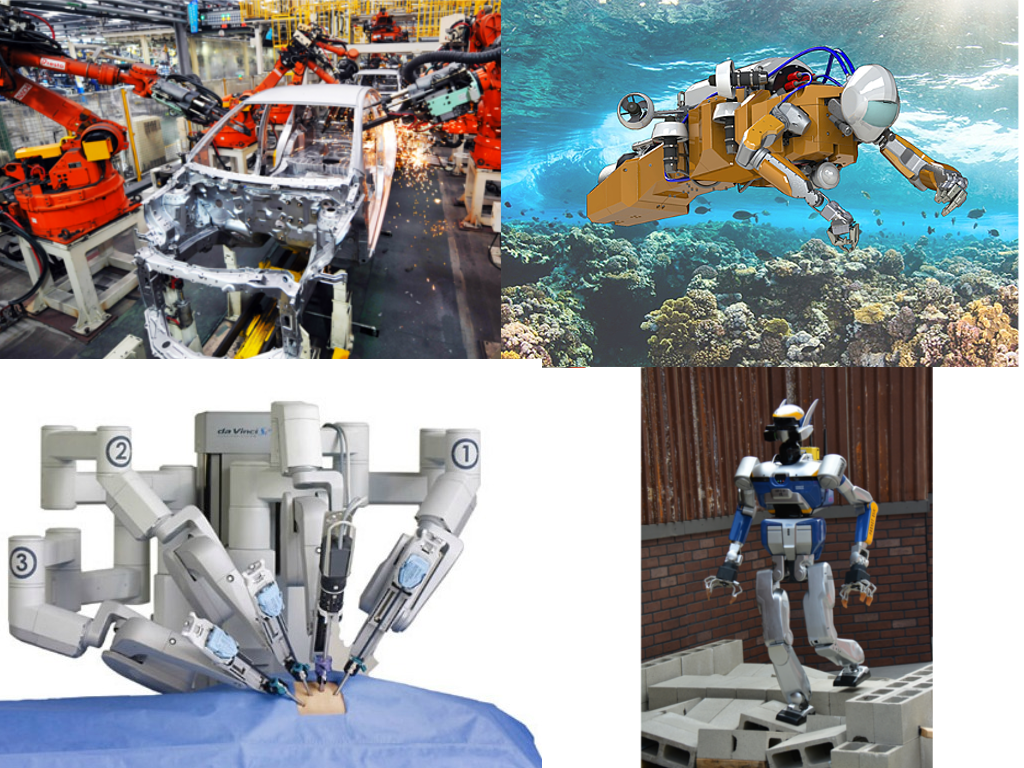
\includegraphics[width=0.9\textwidth]{various-tasks.png}
  \caption{Various robots doing various tasks}
  \label{fig:various}
\end{figure}

The DARPA Robotics Challenge has brought some light on the humanoid robots.
This competition brought together a large scope of robotics groups from universities, laboratories and private companies around a common goal: Make a robot succeed in several challenges without any human physical intervention.
The robots were expected to drive a car, open a door, climb stairs, cross debris, drill a hole in a wall, etc.
All those tasks can usually be broken down into sets of elementary tasks in human language.
Some typical examples of tasks for a robot can be "Put hand in contact with target", "Put foot on next step", "Avoid collision with that object", "Maintain stability" or "Look in that direction".
As is, those tasks do not mean anything for the robot.
A robot is made of a collection of bodies that are linked together by joints, that are actuated by motors.
A robots configuration consists of the position and orientation of its base body, and the configuration of each of its joints.
Satisfying a task requires that the joints of the robot reach a configuration for which the task is satisfied.
The action of satisfying a task comes down to moving from an initial configuration to a goal configuration, figuring out the trajectory to follow and actually following it are the jobs of the trajectory generation and the control of the robot.
Those are by themselves some complete fields of robotics, and they have one thing in common, they both need to be given an initial configuration, a final configuration and sometime some intermediate configurations.
Finding those configurations is the job of what we call the Posture Generation (PG), which is the main topic of this dissertation.
There are two types of robots. The fixed-base robots and the mobile robots.
The first type of robots have fixed basis, which mean that the area that they can reach is predefined by their geometry and are usually fully-actuated.
Which means that the robot has as many dof as actuators, Thus, for any joint configuration, a unique robots position is achieved.
On the contrary, mobile robots are under actuated, which means that the robot has more dof than actuators.
Each link of the robot is actuated, but the position of the basis of the robot is the result of the configuration of the joints and of the contacts that the robot makes with the environment.
A mobile robot's position depends on the location of its contacts with the environment.
For biped robots evolving on a flat surface, a footstep planner can be used to decide of the sequence of steps to take so the robot can walk to its goal.

Humanoid robots are expected to move and achieve tasks in ways similar to humans.

On flat surfaces, they can walk based on a cyclic motion and the locations of footsteps can be generated by a footstep planner using some simplified models to maintain the robots stability.
In cumbersome and unstructured environments, we humans move in a non-gaited acyclic way: we choose appropriate parts of our body to create contacts with the surrounding environment in order to support the motion of the remaining parts while avoiding obstacles.
A whole motion is a sequence of contact creations and releases.

Since we are biped, we mostly use our feet to move.
As the environment becomes more difficult to cross, hands may come into play together with feet to help with the motion.
Narrow passages may even require other parts of our body (knees, elbows, back...) to make contact in order to support the motion.

In the past few years, our team has dedicated considerable efforts in proposing a general multi-contact motion planner to solve such cases of non-gaited acyclic planning.
Given a humanoid robot, an environment, a start and a final desired postures, the planner generates a sequence of contact stances allowing any part of the humanoid to make contact with any part of the environment to achieve motion towards the goal.
The planner's role is to grow a tree of contact stances iteratively, from a given posture, it tries to removes one of its contacts or to add a new one.
The tree grows, following some heuristics until the solution is reached.
A typical experiment with a HRP-2 robot achieving such an acyclic motion is presented in~\cite{escande:iser:2008}, and the planner is thoroughly described in~\cite{escande:ras:2013}.
Extensions of this multi-contact planner to multi-agent robots and objects gathering locomotion and manipulation are presented in~\cite{bouyarmane:ar:2012}, and preliminary validations with some DARPA challenge scenarios, such as climbing a ladder, ingress/egress a utility car or crossing through a relatively constrained pathway are presented in~\cite{bouyarmane:humanoids:2012}.
\cite{hauser:issr:2007} presents a different approach to multi-contact planning based on probabilistic roadmap and random sampling of the configuration space.
Another way of planning a multi-contact scenario, which is actually the most popular, is to do it by hand, the user chooses iteratively which contacts to add and remove until the goal is reached.

Planning the sequence of contacts to achieve is a necessary step in devising a motion for a robot.
Once the key stances of the motion have been identified by the planner, they can be used by the controller or the trajectory planner and finally the motion can be achieved by the robot.

All the aforementioned planning method rely on the fact that we have a tool to decide if a proposed set of contact is feasible or not for the robot.
The tool used for finding a robot configuration that satisfies a set of constraints like the geometric constraints of contact is called a "Posture Generator" (PG) and the development of that tool is the main topic of this dissertation.

The mission of a posture generator is, for a poly articulated system, to find a configuration so that the system satisfies a set of constraints.
For simple systems, with simple constraints, like a 6 dof robotic arm having to reach a point with its end effector, some closed-form expressions can usually be devised.
But computing robot configuration to meet the requirements of a given set of tasks, within a viable state, is a recurrent problem whose complexity grows with that of the robot.
When the robotic problem studied becomes too complex for closed-form formulas, it is formulated as a non-linear optimization program and solved using state of the art optimization algorithms.

Because it is a key element for many robotics application, the posture generator is a very important element of any robotics framework.
It needs to be efficient at finding a solution when one exists and at figuring when a problem is not feasible.
The speed of generating a multi-contact sequence is directly related to the quality of the posture generator.

If we consider a problem of posture generation on a mobile robot with $n$ joints, the configuration space of the joints of the robot is $\mathbb{R}^n$ and the configuration space of the position and orientation of its base body is $SE(3) = \mathbb{R}^3\times SO(3)$.
Thus, the variable that describes the configuration of the robot in the optimization problem lives in $\mathbb{R}^3\times SO(3) \times \mathbb{R}^n$.
$SO(3)$ is by nature a non-Euclidean manifold, it cannot be parameterized on an open subset of Euclidean space without having to deal with problems of gimbal lock.
The gimbal lock is a singularity that happens when parameterizing $SO(3)$ on $\mathbb{R}^3$, with Euler angles, for example, and when two axis of rotation become aligned, in that situation, 2 elements of the parameterization correspond to the same rotation.
Thus, one degree of freedom is lost.
It is possible to parameterize $SO(3)$ without having to face singularities by parameterizing it over another non-Euclidean manifold.
The most common ones being the unit quaternion space $\mathcal{H}$, and the $3\times 3$ rotation matrix.
Most of the solvers available make the assumption that the search space is Euclidean, which makes is complicated to use quaternion or rotation matrix efficiently.
To put it simply, for the unit quaternion parameterization, a variable on $SO(3)$ is represented by 4 variables and an equality constraint

\begin{equation}
  q\in\mathcal{H} = \{q\in\mathbb{R}^4:||q||=1\}
\end{equation}

Although, there exist some emerging methods and algorithms to solve optimization problems on non-Euclidean manifolds with no substantial extra cost and guaranteeing a good coverage of the manifolds without facing parameterization singularities and with the minimal number of parameters.
One of the particularity in our approach of posture generation is that we develop, extend and use one such optimization algorithm on manifolds to solve robotics problems.

\subsection{Posture Generation}
\label{sub:posture_generation}

\subsection{Optimization}
\label{sub:optimization}

\section{Problem Definition}
\label{sec:problem_definition}

We consider a robot $\mathit{R}$ with $n$ degrees of freedom (dof), its joint configuration can be described by a point on

\section{From Inverse Kinematics to Posture Generation}
\label{sec:from_inverse_kinematics_to_posture_generation}

The problem of finding a configuration of a poly articulated system to satisfy some geometric constraints has been widely studied for decades under the name of Inverse Kinematics (IK).
IK is an important tool in many fields like robotics, computer graphics and animation.




%%%%%%%%%%%%%%%%%%%%%%%%%
%  SECTION FORMULATION  %
%%%%%%%%%%%%%%%%%%%%%%%%%

\section{Formulation}

Here we present the basic formulation of a PG problem.

The free-flyer, the articular space and the forces being the usual variables.

Presentation of all the constraints and their formulation
\begin{itemize}
  \item Joint limits
  \item Auto-collision
  \item Collisions with environment
  \item Contacts with environment
  \item Stability
  \item Torque limits
\end{itemize}


%*******************************************************************************
%*********************************** First Chapter *****************************
%*******************************************************************************

\chapter{Numerical Optimization: Introduction}
\label{chapter:optimization}

\nomenclature[x-R]{$\mathbb{R}$}{Real space}
\nomenclature[x-S]{$\mathit{S}$}{Variable space}
\nomenclature[x-M]{$\mathcal{M}$}{A Manifold}
\nomenclature[x-T]{$T_x\mathcal{M}$}{The tangent space of manifold $\mathcal{M}$ at point x}
\nomenclature[a-F]{$F$}{The set of linearized feasible directions}
\nomenclature[a-f]{$f$}{Objective function}
\nomenclature[a-c]{$c_i$}{Constraint function}
\nomenclature[a-x]{$x$}{Optimization variable}
\nomenclature[a-xstar]{$x^*$}{Solution of the optimization problem}
\nomenclature[a-E]{${E}$}{Set of index for which constraints are equality constraints}
\nomenclature[a-I]{${I}$}{Set of index for which constraints are inequality constraints}
\nomenclature[x-L]{$\mathcal{L}(x,\lambda)$}{Lagrangian function of the optimization problem}
\nomenclature[G-o]{$\Omega$}{Feasible set}
\nomenclature[z-st]{s.t.}{subject to}
\nomenclature[z-KKT]{KKT}{Karush-Kuhn-Tucker first order optimality conditions}
\nomenclature[z-LICQ]{LICQ}{Linear Independence Constraints Qualification}
\nomenclature[z-QP]{QP}{Quadratic Programming}
\nomenclature[z-IQP]{IQP}{Inequality constrained Quadratic Programming}

\ifpdf
    \graphicspath{{Chapter1/Figs/Raster/}{Chapter1/Figs/PDF/}{Chapter1/Figs/}}
\else
    \graphicspath{{Chapter1/Figs/Vector/}{Chapter1/Figs/}}
\fi

\section{List of contributions}
\begin{itemize}
  \item \sout{Introduction to optimization}
  \item \sout{Notions of unconstrained optimization}
  \item \sout{Notions of Constrained Optimization}
  \item \sout{KKT}
  \item Line Search
  \item Trust Region
  \item Filter
  \item Merit function
  \item SQP
  \item Restoration phase
  \item \sout{Hessian Approximation: BFGS, SR1}
\end{itemize}

%********************************** First Section *********************************
\section{Introduction}
In modern science, optimization has a very important place.
Mechanical engineers optimize the shape of stuctural parts.
Investors optimize the profit of a portfolio while minimizing the risks of loss.
Chemists optimize the efficiency and speed of reactions.
When it comes to robotics, optimization is everywhere.
From the design of a robot to its actuation.
Any positioning of a robot requires the computation of the articular parameters of each joint of the robot, finding such parameters might be possible by using analytical methods for very simple robots, but for robots as complex as humanoid robots, it is not possible.
Most often, an optimization process is used.

The goal of an optimization algorithm is to find an optimal solution $x^*$ to a problem.
Optimal in the sense that the solution is an optimum of a given objective function $f$.
And solution of a problem in the sense that is satisfies a set of $m$ constraints $\{c_i,\ i\in [1,m]\}$.
Both the constraints and the objective function are defined on the variable space $\mathit{S}$, which is the space in which the variable $x$ lives and in which we search a solution $x^*$ to our problem.

In order to present the principles of optimization, in this chapter we will always consider that the variable space is $\mathit{S}=\mathbb{R}^n$.
We first consider unconstrained problems, that do not have any constraint and that only goal is to minimize a cost function.
That type of problem will not be used in the rest of our dissertation, therefore, we will just present them shortly.
We will then focus on constrained optimization problems and the numerous methods used in their resolution.
We will particularly detail one specific constrained problem resolution algorithm that is the Sequential Quadratic Program(SQP).
The extension of those methods to solving problems on more complex variable spaces that are the non Euclidean manifolds will be the topic of a further chapter of this dissertation.

\section{Unconstrained Optimization}

An unconstrained optimization problem consists in minimizing an objective function without any constraint.
This problem that we denote $\mathcal{P}$ can be formulated as follows:

\begin{equation}
  \min_{x\in\mathbb{R}^n}\ {f(x)}
\label{eq:unconstrainedOptim}
\end{equation}

In order to solve this problem, we want to design an iterative algorithm that, starting from an initial guess $x_0$, will converge toward the solution $x^*$.
The objective function is not necessarily completely known.
In the sense that we cannot always have an explicit formula, often, the function $f$ is computed by another program that is able to compute $f(x)$, $\nabla_x f(x)$ and sometimes $\nabla_{xx} f(x)$ for a given value of $x$.
In order to have an efficient algorithm, we want to avoid any unnecessary computation of $f(x)$ and its derivatives.
We will denote the values taken by $x$ along the iterations as $x_0$, $x_1$, $x_2$,\ldots $x_i$.
And $f(x_i)$ is denoted $f_i$.

Since our knowledge of the objective function is only partial, it would not be possible to guarantee that a point $x^*$ is a global solution:

\begin{equation}
  \text{$x^*$ is a global solution of $\mathcal{P}$ on $\mathit{S}$ } \equiv \forall x \in \mathit{S}, f(x^*) \leq f(x)
\end{equation}

Though, we can find a local solution $x^*$ of $\mathcal{P}$ (a local minimizer of $f$) such that:

\begin{equation}
  \text{There exist a neighborhood } \mathit{N}\text{ of }x^*\text{ such that
  }\forall x\in \mathit{N}, \ f(x^*) \leq f(x)
\end{equation}

That is the kind of solution that we are looking for and that our algorithms should find.

Under the assumption that the objective function is smooth and sufficiently continuous ($\mathcal{C}_2$), then we have the following sufficient conditions for the optimality of $x^*$ as presented in \cite{nocedal:book:2006}:

\begin{theorem}
  If $\nabla^2f$ is continuous in an open-neighborhood of $x^*$ and that $\nabla f(x^*)=0$ and $\nabla^2 f(x^*)$ is positive definite.
  Then $x^*$ is a strict local minimizer of $f$.
  \label{optimalityTheorem}
\end{theorem}

%\subsection{Globalization methods}

%During the resolution of an optimization problem, the algorithm will generate a
%sequence of iterates $x_k$ starting from the initial iterate $x_0$ (Which is
%usually provided by the user). During the step $k$ of the optimization process,
%the solver, the current point is $x_k$ and we try to find $x_{k+1}$ such that
%$f(x_{k+1}) < f(x_k)$. There are several strategies to do that but we will only focus
%on 2 of them that are the most popular, the line-search and trust-region
%methods.

%\subsubsection{The Line-Search Strategy}
%In the Line-Search strategy, given a point $x_k$, a descent direction $p_k$ from this
%point is chosen and then a length of step is calculated to minimize the
%following 1-dimentional problem:
%\begin{align}
  %\min_{\alpha \in \mathbb{R}^+} f(x_k + \alpha.p_k)
%\label{eq:lineSearchNLP}
%\end{align}

%Once the best value of $\alpha$ has been found, the next iterate is computed:
%$x_{k+1} = x_{k} + \alpha p_k$ and the same process is repeated until a
%satisfying solution is found.

%It is not always necessary to find the optimal value of $\alpha$, especially if
%that is expensive. Indeed, $\alpha$ is only used to calculate the next iterate,
%from which another $p_k$ and $\alpha$ will be calculated. And in the end, the
%imprecision on the computation of $\alpha$ will be errased in the other steps of
%the resolution.

%There are several ways to choose a descent direction from an iterate $x_k$. The
%most obvious one is probably the steepest descent direction $-\nabla f_k$. This
%method provides the direction along which f decreases most rapidly and only
%requires the evaluation of the first derivative of $f$, but that method can
%become extremely slow on complicated problems. Another popular approach is the
%Newton method, in which the objective function is approximated to the second
%order

%\begin{equation}
  %f(x_k+p) = f_k + p^T\nabla f_k + p^T\nabla^2f_k p
%\end{equation}

%Then the chosen descent direction is the optimum of that approximated function,
%the Newton direction.
%\begin{equation}
  %p^N_k = -(\nabla^2 f_k)^{-1} \nabla f_k
%\end{equation}
%The choice of this descent direction implies that the $\nabla^2f_k$ is positive
%definite, in which case an adaptation of the definition of $p_k$ is required. Or
%an approximation $B_k$ of $\nabla^2f_k$ that guaranties definite positiveness can be
%used. For example, the symmetric-rank-one(SR1) formula and the BFGS(Broyden,
%Fletcher, Goldfarb, Shanno) formula. Then the step becomes

%\begin{equation}
  %p_k = -B_k^{-1}\nabla f_k
%\end{equation}

%\subsubsection{The Trust-Region Strategy}
%The Trust-Region Strategy works in an opposite way than the line-search one in
%the sense that during a line-search step, a direction is chosen, and based on
%that direction, a step-length is chosen. Whereas with a Trust-Region approach, a
%maximum step-length is chosen, and based on it, the descent direction and lenght
%are chosen.
%The principle of the trust region is that along the optimization process, a
%model of the problem is constructed and enriched at every step and at each step,
%the next iterate is the optimum of the model, with the constraint that the step
%to get there lies inside the trust-region. For example, let us considere that
%the trust region is a sphere of center $x_k$ and radius $\rho_k$, then the
%constraint on $p_k$ is $\|p_k\| \leq \rho_k$. A usual model to take for the
%objective function is the quadratic model with approximated Hessian
%\begin{equation}
  %m_k(p) = f(x_k+p) = f_k + p^T\nabla f_k + p^TB_k p
%\end{equation}
%And the optimization problem to solve at each step of the optimization is

%\begin{align}
  %\min_{p} & \quad f_k + p^T\nabla f_k + p^TB_k p \nonumber\\
%\text{s.t.}&
%\quad \|p\| \leq \rho_k
%\label{eq:trustRegionNLP}
%\end{align}

%Once the solution $p_k$ to this quadratic problem is found, its quality is
%estimated by evaluating the value of $f(x_k+p_k)$. If the actual decrease of $f$
%is satisfying (compared to the decrease predicted by the model) then the step is
%accepted and the size of the trust-region can be increased. Otherwise, the step
%is refused, the trust-region radius is reduced and a new step from $x_k$ is
%computed on that smaller trust region.

\section{Constrained Optimization}

Solving a constrained optimization problem consists in minimizing a cost function while satisfying a set of constraints.

A general formulation for such problems (that we denote $\mathcal{P}$) is:

\begin{equation}
  \label{formulation_NLCP}
  \mathcal{P} \equiv
  \left\{
  \begin{array}{l}
    \min\limits_{x\in\mathbb{R}^n}{f(x)}\\
    \text{ s.t. }
    \left\{
    \begin{array}{l}
      c_i(x) = 0,\ \forall i\in{E}\\
      c_i(x) \geq 0,\ \forall i\in{I}\\
    \end{array}
    \right.
  \end{array}
  \right.
\end{equation}

Where $f$ and $c_i$ are real valued functions on a subset of $\mathbb{R}^n$.
$f$ is the objective function. And $c_i$ are the constraint functions.
${I}$ and ${E}$ are sets of index such that $c_i,\ i\in{E}$ are the equality constraints, and $c_i,\ i\in{I}$ are the inequality constraints.

We define the feasible set $\Omega$ that contains all the feasible points (points satisfying the constraints) of $\mathcal{P}$ \ref{formulation_NLCP}.

\begin{equation}
  \Omega = \left\{ x\in \mathbb{R}^n:\ \forall i\in {E},\ c_i=0,\ \forall i\in{I},\ c_i \geq0\right\}
\end{equation}

The formulation \ref{formulation_NLCP} can then be rewritten as:
\begin{equation}
  \label{formulation_NLCP_compact}
  \mathcal{P} \equiv \min_{x\in\Omega}{f(x)}
\end{equation}

In the general case, the problem \ref{formulation_NLCP_compact} has multiple local solutions.
And finding the global minimizer of $f$ in $\Omega$ is a difficult problem that we do not treat in this thesis.
Our goal is to find a local minimizer $x^*$ of $f$ in $\Omega$.

\subsection{Optimality conditions}

\paragraph{First-Order Optimality Conditions}

The First Order Optimality Condition (Karush-Kuhn-Tucker Condition) is a necessary condition verified by all solutions of problem \ref{formulation_NLCP}.

We introduce the Lagrangian function of \ref{formulation_NLCP}:
\begin{equation}
  \mathcal{L}(x,\lambda) = f(x) + \sum_{i\in E\cup I}\lambda_i c_i(x)
\end{equation}

Any given constraint $c_i$ is said to be active at $x$ if $c_i(x)=0$.
In particular, for any feasible point $x$, all equality constraints $c_i,\ i\in E$ are active. 
An inequality constraint $c_i,\ i\in I$ is inactive if $c_i(x)>0$ and active if $c_i(x) = 0$

\begin{definition}  
  \label{active_set}
  The active set $\mathit{A}(x)$ at a feasible point $x$ is the set of all the indexes of active constraint.
  \begin{equation}
    \mathit{A}(x)=E\cup\{i\in I: c_i(x) = 0\}
  \end{equation}
\end{definition}

Most optimization algorithms make the assumption that at the solution, the constraints satisfy the Linear Independence Constraints Qualification (LICQ)

\begin{definition}
  Given a point $x$ and an active set $\mathit{A}(x)$, the LICQ holds if the set of active constraint gradient $\{\nabla c_i(x),\ i\in \mathit{A}(x)\}$ is linearly independent
\end{definition}

In particular, if any gradient of a constraint is null, then the LICQ does not hold. 
The LICQ should be taken into account during the formulation of a problem.

\begin{theorem}(First-Order Necessary Conditions)\\
  \label{KKT_conditions}
  Suppose that $x^*$ is a local solution of \ref{formulation_NLCP}, that the functions $f$ and $c_i$ are continuously differentiable, and that the LICQ holds at $x^*$.
  Then there is a Lagrange multiplier vector $\lambda^*$, with components $\lambda_i^*$, $i\in E\cup I$, such that the following conditions are satisfied at $(x^*,\lambda^*)$
  \begin{equation}
  \begin{array}{ll}
    \nabla_x\mathcal{L}(x^*,\lambda^*) = 0 &, \\
    c_i(x^*) = 0 &,\ \forall i\in E\\
    c_i(x^*) \geq 0 &,\ \forall i\in I\\
    \lambda_i^* \geq 0 &,\ \forall i\in I\\
    \lambda_i^* c_i(x^*)=0 &,\ \forall i \in E\cup I\\
  \end{array}
  \end{equation}
\end{theorem}

In many cases, the main goal of an optimization algorithm is to find a point that satisfies the KKT conditions.

\paragraph{Second-Order Optimality Conditions}

\begin{definition}
  Given a feasible point $x$, and the active set $\mathit{A}(x)$, the  set of linearized feasible directions $F(x)$ is:
  \begin{equation}
    F(x)=\left\{d\left|
        \begin{array}{ll}
          d^T\nabla c_i(x) = 0&,\ \forall i\in E \\
          d^T\nabla c_i(x) \geq 0&,\ \forall i\in \mathit{A}(x)\cap I \\
        \end{array}
        \right.
    \right\}
  \end{equation}
\end{definition}

And at a KKT solution $(x^*,\lambda^*)$ the critical cone $C(x^*, \lambda^*)$ is:

\begin{equation}
  C(x^*,\lambda^*) = \{w\in F(x^*)|\nabla c_i(x^*)^Tw=0, \forall i\in\mathit{A}(x^*)\cap I \text{ with } \lambda_i^*>0\}
\end{equation}

The critical cone contains the linearly feasible directions for which it is not clear from first derivative information alone if $f$ will increase or decrease.

Once the KKT condition is reached for a point $(x^*, \lambda^*)$.
For a direction $w$ of $F(x^*)$ for which $w^T\nabla f(x^*)=0$, it is impossible to tell from first derivative information only, if an increment in this direction will have a positive effect on the problem resolution.
Thus it is possible that the KKT constaint is not enough to determine if a point is a solution or just a stationary point.

The Second-Order Sufficient Conditions allow to discriminate local solutions from stationary points:

\begin{theorem}
  Suppose that for some feasible point $x^*\in \mathbb{R}^n$ there is a Lagrange multiplier vector $\lambda^*$ such that the KKT conditions are satisfied. Suppose also that
  \begin{equation}
    w^T\nabla_{xx}^2\mathcal{L}(x^*,\lambda^*)w>0,\ \forall w\in C(x^*,\lambda^*),\ w\neq 0
  \end{equation}
  Then $x^*$ is a strict local solution for \ref{formulation_NLCP}
\end{theorem}

In particular, this condition is always verified if $\nabla_{xx}^2\mathcal{L}(x^*,\lambda^*)$ is positive definite.

\section{Resolution of a Non Linear Constrained Optimization Problem}

In the previous section, we presented some theoretical tools to describe the solution of an NLCP that only use the derivative terms of order one and two of the problem's functions.
Here we present some methods for acually solving such problems.
There exists many different algorithms to solve an NLCP.
But all have in common to be iterative processes.
In which we start from an initial guess $x_k$ for $x^*$.
From the first and (sometimes) second-order informations on the functions $f$ and $c_i$ that constitute the problem \ref{formulation_NLCP}, we find a suitable increment $z$ such tha $x_k+z$ is closer to the solution than $x_k$.
And we iterate that operation until a point $x_k$ sufficiently close to a solution is found.
By sufficiently close to a solution we mean that this point satisfies the optimality conditions with a good enough precision.

The resolutions algorithms differ mostly by the method chosen to generate a satisfactory increment $z$. We will list here some of the most popular methods:

\paragraph {The penalty method} combines the cost and constraints function in a penalty function that, as its name indicates, penalizes the violation of constraints, without completely proscribing it.
The penalty function can be written as follows, using the notation $[y]^- = \max\{0, -y\}$:

\begin{equation}
  \label{penalty_function}
  p(\mu, x) = f(x) + \mu \sum_{i\in E}|c_i(x)| + \mu \sum_{i\in I} [c_i(x)]^-
\end{equation}

With this approach, an unconstrained optimization approach can be used.
The minimum of $p(\mu,x)$ varies with the penalty parameter $\mu$.
By increasing $\mu$ to $\infty$, we penalize the violation of the constraints with increasing severity until reaching a solution $x^*$.

\paragraph{The interior point method} generates steps by solving a relaxed constrained problem where slack variables are introduced to relax inequality constraints.
The problem to solve only contains equality, boundary constraints and a cost function a cost function that prevents the slack variables from getting too close to 0:

\begin{equation}
  \min_{x,s}{ f(x)- \mu\sum_{i\in I} \log(s_i)}
  \text{ subject to }
  \left\{
    \begin{array}{l}
     c_i = 0,\ i\in E\\
     c_i - s_i = 0,\ i\in I\\
     s_i \geq 0,\ i\in I
  \end{array}
  \right.
\end{equation}

\paragraph{The Sequential Quadratic Programming (SQP)} is a method in which, at each iterate $(x_k, \lambda_k)$, the increment $z$ is found by solving a Quadratic Programming (QP).
The QP is an approximation of the KKT conditions \ref{KKT_conditions} of the actual problem \ref{formulation_NLCP} to the first order:

\begin{equation}
  \label{approx_QP}
  \begin{array}{ll}
    \min\limits_{z\in \mathbb{R}^n}{} & \frac{1}{2}z^T\nabla_{xx}^2\mathcal{L}(x_k, \lambda_k)z + \nabla f(x_k)^Tz \\
    \text{subject to } & \nabla c_i(x_k)^Tz+c_i(x_k)=0,\ i\in E \\
                       & \nabla c_i(x_k)^Tz+c_i(x_k)\geq 0,\ i\in I
  \end{array}
\end{equation}

Given $z^*$ the solution of \ref{approx_QP}, it can be tempting to directly take the next iterate as $x_{k+1} = x_k + z^*$.
But using that method as is can be problematic as the length of the iterate needs not be bounded.
Thus it is possible to generate a very large step that satisfies the QP.
The QP only approximates the original problem locally.
So taking a too big step can get us further from the solution than we previously were.
To paliate to that issue, mainly two methods are used:
\begin{itemize}
  \item The line-search method: The solution $z$ of \ref{approx_QP} is viewed as a direction and we search a parameter $\alpha\in [0;1]$ so that the next iterate $x_k + \alpha z$ is optimal for the original problem.
  \item The trust-region method adds a set of bound constraints to the QP \ref{approx_QP}. So that the length of the step is limited by the trust-region. The size $\rho$ of the trust region is modified along the iterations based on the estimated quality of the QP approximation. In that case, the QP becomes:
\begin{equation}
  \label{approx_QP_TR}
  \begin{array}{ll}
    \min\limits_{z\in \mathbb{R}^n}{} & \frac{1}{2}z^T\nabla_{xx}^2\mathcal{L}(x_k, \lambda_k)z + \nabla f(x_k)^Tz \\
    \text{subject to } & \nabla c_i(x_k)^Tz+c_i(x_k)=0,\ i\in E \\
                       & \nabla c_i(x_k)^Tz+c_i(x_k)\geq 0,\ i\in I\\
                       & |z|<\rho
  \end{array}
\end{equation}
\end{itemize}

\section{Sequential Quadratic Programming}
\label{sec:sequential_quadratic_programming}

The Sequential Quadratic Programming method is one of the most effective method to solve small and large scale non-linear constrained optimization problems.
It has the upper hand on other methods mostly when solving problem with highly non-linear constraints.

\subsection{Principle}
\label{sub:principle}

As we stated before, the main idea behind the SQP approach it to solve a subproblem that approximate linearly to the first order the KKT conditions.
For simplicity, we considere a problem without inequality constraints.
We denote $C$ the vector of equality constraints.
We denote $z_x$ and $z_\lambda$ the increments on $x$ and $\lambda$ respectively.
\begin{equation}
  \begin{array}{l}
    x_{k+1} = x_k + z_x\\
    \lambda_{k+1} = \lambda_k+z_\lambda\\
  \end{array}
\end{equation}

The problem is the following:
\begin{equation}
  \begin{array}{l}
    \min\limits_{x\in\mathbb{R}^n}{f(x)} \\
    \text{ subject to } C(x) = 0
  \end{array}
\end{equation}

Its KKT conditions are:
\begin{equation}
  \label{KKT_equ}
  \left\{
\begin{array}{ll}
  \nabla_x\mathcal{L}(x^*,\lambda^*) = 0\\
  C(x^*) = 0\\
\end{array}
\right.
\end{equation}

We denote with a subscript $y_k$ the value of the quantity $y$ evaluated at point $(x_k, \lambda_k)$.

The first order linearization of \ref{KKT_equ} gives:

\begin{equation}
  \label{KKT_1st_order}
  \begin{array}{l}

  \left\{
\begin{array}{l}
  \nabla_{xx}^2\mathcal{L}_k z_x + \nabla_{x\lambda}^2\mathcal{L}_k z_\lambda + \nabla_x\mathcal{L}_k  = 0\\
  \nabla_x C_k z_x + C_k = 0\\
\end{array}
\right. \\
\text{which is equivalent to:}\\
  \left\{
\begin{array}{l}
  \nabla_{xx}^2\mathcal{L}_k z_x + \nabla_{x}C_k (\lambda_k + z_\lambda) = - \nabla_{x}f_k\\
  \nabla_x C_k z_x = - C_k \\
\end{array}
\right. \\
\text{Or in matrix form:}\\
  \begin{pmatrix}
      \nabla_{xx}^2\mathcal{L}_k & \nabla_x C_k\\
      \nabla_x C_k & 0\\
  \end{pmatrix}
  \begin{pmatrix}
      z_x\\
      \lambda_{k+1}\\
  \end{pmatrix}
  =
  \begin{pmatrix}
      - \nabla_{x}f_k\\
      - C_k\\
  \end{pmatrix}
  \end{array}
\end{equation}

Solving this problem actually is equivalent to solving a QP problem of the following form:

\begin{equation}
  \begin{array}{ll}
    \min\limits_{z_x} &f_k + \nabla_x f_k ^T z_x + \frac{1}{2} z_x^T\nabla_{xx}^2\mathcal{L}_k z_x \\
    \text{s.t.} & \nabla_x C_k^T z_x + C_k = 0\\
  \end{array}
\end{equation}

The unique solution of this problem satisfies the following matrix equality:

\begin{equation}
  \begin{pmatrix}
      \nabla_{xx}^2\mathcal{L}_k & -\nabla_x C_k\\
      \nabla_x C_k & 0\\
  \end{pmatrix}
  \begin{pmatrix}
      z_x\\
      l_k\\
  \end{pmatrix}
  =
  \begin{pmatrix}
      - \nabla_{x}f_k\\
      - C_k\\
  \end{pmatrix}
\end{equation}

Note that this problem has a solution if the following assumptions hold:
\begin{itemize}
  \item The constraint Jacobian $\nabla_x C_k$ has full rank.
  \item The matrix $\nabla_{xx}^2\mathcal{L}_k$ is positive definite on the tangent space of the constraints:\\ $d^T\nabla_{xx}^2\mathcal{L}_k d \geq 0,\ \forall d\neq 0$ such that ${\nabla_x C_k}^T d = 0$.
\end{itemize}

Therefore, the problem raised by the linearization of the KKT conditions to the first order can be solved as a QP problem.
Denoting the solution of the QP problem $(z_x, l_k)$, the solution to \ref{KKT_1st_order} is given by

\begin{equation}
  \begin{pmatrix}
      z_x\\
      \lambda_{k+1}\\
  \end{pmatrix}
  \leftarrow
  \begin{pmatrix}
      z_x\\
      -l_k\\
  \end{pmatrix}
\end{equation}

This development can easily be extended to treat the case of problems constrained with inequality constraints:

\begin{equation}
  \min_{x\in\mathbb{R}^n}{f(x)} \text{ subject to }
  \left\{
  \begin{array}{l}
    c_i(x) = 0,\ \forall i\in{E}\\
    c_i(x) \geq 0,\ \forall i\in{I}\\
  \end{array}
  \right.
\end{equation}

By solving the following Inequality-constrained Quadratic Problem(IQP) system at each iteration:

\begin{equation}
  \label{IQP}
  \begin{array}{ll}
    \min\limits_{z_x} &f_k + \nabla_x f_k ^T z_x + \frac{1}{2} z_x^T\nabla_{xx}^2\mathcal{L}_k z_x \\
    \text{s.t.} & \nabla_x {c_i}_k z_x + {c_i}_k = 0 ,\ \forall i\in E\\
                & \nabla_x {c_i}_k z_x + {c_i}_k \geq 0 ,\ \forall i\in I\\
  \end{array}
\end{equation}

The main difficulty in solving that QP \ref{IQP} comes from finding the optimal active set $\mathit{A}_k$.
It is a necessary but costly operation.
Especially when starting from a random active set $\mathit{A}_0$.
The process is mostly based on a try and guess approach guided by euristics(that may vary with different resolution algorithms).

To find the optimal active set, the QP starts from a random active set $\mathit{A}_0$ ignore the non-active constraints and try to solve the QP with the remaining active constraints.
At a step $k$ of the resolution of the IQP, all the constraints in the active set $\mathit{A}$ are treated as equality constraints and the others are simply ignored, the QP to solve becomes:

\begin{equation}
  \text{EQP} \equiv \left\{
  \begin{array}{ll}
    \min\limits_{z_x} &f_k + \nabla_x f_k ^T z_x + \frac{1}{2} z_x^T\nabla_{xx}^2\mathcal{L}_k z_x \\
    \text{s.t.} & \nabla_x {c_i}_k z_x + {c_i}_k = 0 ,\ \forall i\in \mathit{A}_k\\
  \end{array}
  \right.
\end{equation}

This EQP is solved, and its solution is checked against the constraints that were previously ignored.
If some of them are violated then the solution is not satisfactory and the active set is updated by adding one or several of the violated constraints to it.
This operation is repeated until there is no more constraints to be added.
Once all the constraints have been adde as active constraints to the EQP, the problem may be overconstrained.
To detect that, the Lagrange multipliers are computed and if some of them do not agree with the KKT conditions of the IQP \ref{IQP}, then one of them is removed from the active set and the resulting EQP is solved, and the process continues until a satisfactory solution is found.
The euristics used to choose which constraints to add or remove from the active set and to avoid cycling between active sets are out of the scope of this dissertation.

Once the SQP gets close to the solution, the set of active constraints should not change much from one iterate $x_k$ to the next one.
It is often useful to initialize the IQP's active set with the optimal active set of the previous iterate: $\mathit{A}_0(x_{k+1})\leftarrow\mathit{A}^*(x_k)$. Then the ${(k+1)}^{th}$ QP starts from an active set close to optimal and can be solved much faster.
That method is called the \textit{warm-start}.

The SQP approach to solving the problem \ref{formulation_NLCP} as presented above leans on the assumption that at each step, the QP generated is feasible,
which requires that the Hessian $\nabla_{xx}^2\mathcal{L}$ is positive definite on the tangent space of the active constraints.
That property is guarantied to hold near the solution, but not when starting from a remote point on a non-convex problem.
To quope with that issue, several methods exist.
In the next few section, we will present the globalisation methods that are the Line Search and Trust Region approaches, they ensure that the QP subproblem is always feasible.
Then we'll present some methods used to choose whether to accept of reject an iterate with the merit function and filter methods.
And finally we will discuss some Hessian approximation methods.

\subsection{Globalization methods}
\label{sub:globalization_methods}

As we stated above, the globalisation phase of an SQP optimization is meant to modify the step generated by the QP resolution in order to improve the the global convergence of the algorithm.
Either by multiplying the step found by the QP with a coefficient $\alpha$ in the Line-Search approach.
Or by bounding the norm of the step found in the QP by adding a boundary constraint on $z$ directly inside of the QP problem.

\subsubsection{The Line-Search Strategy}
In the Line-Search strategy, starting from a current iterate $x_k$ with a QP generated step $z$ solution of the linearized problem. We search a coefficient $\alpha$ such that $x_{k+1}=x_k+\alpha z$ is satisfactory.
A usual way to decide if a point is satisfactory is to use a Merit function.
A Merit function is somewhat similar to a penalty function.
In the sense that it estimates the quality of a point from the value of the cost function penalized by the violation of the constraints.
A typical merit function for a problem with only equality constraints can be written as:
\begin{equation}
  M(x,\mu) = f(x)+\mu \|c(x)\|_1
\end{equation}

If inequality constraints are present, a simple penalty function like \ref{penalty_function} would not be satisfactory because of the non-smoothness of the operator $[.]^-$.
To avoid that problem, slack variables can come in handy to replace the inequality constraints in the problem as follows:

\begin{equation}
  c_i(x)\geq 0\ \equiv
  \left\{
  \begin{array}{l}
    c_i(x)-s_i=0\\
    s_i\geq 0
  \end{array}
  \right.
\end{equation}


given a point $x_k$, a descent direction $p_k$ from this
point is chosen and then a length of step is calculated to minimize the
following 1-dimentional problem:
\begin{align}
  \min_{\alpha \in \mathbb{R}^+} f(x_k + \alpha.p_k)
\label{eq:lineSearch}
\end{align}

Once the best value of $\alpha$ has been found, the next iterate is computed:
$x_{k+1} = x_{k} + \alpha p_k$ and the same process is repeated until a
satisfying solution is found.

It is not always necessary to find the optimal value of $\alpha$, especially if
that is expensive. Indeed, $\alpha$ is only used to calculate the next iterate,
from which another $p_k$ and $\alpha$ will be calculated. And in the end, the
imprecision on the computation of $\alpha$ will be errased in the other steps of
the resolution.

There are several ways to choose a descent direction from an iterate $x_k$. The
most obvious one is probably the steepest descent direction $-\nabla f_k$. This
method provides the direction along which f decreases most rapidly and only
requires the evaluation of the first derivative of $f$, but that method can
become extremely slow on complicated problems. Another popular approach is the
Newton method, in which the objective function is approximated to the second
order

\begin{equation}
  f(x_k+p) = f_k + p^T\nabla f_k + p^T\nabla^2f_k p
\end{equation}

Then the chosen descent direction is the optimum of that approximated function,
the Newton direction.
\begin{equation}
  p^N_k = -(\nabla^2 f_k)^{-1} \nabla f_k
\end{equation}
The choice of this descent direction implies that the $\nabla^2f_k$ is positive
definite, in which case an adaptation of the definition of $p_k$ is required. Or
an approximation $B_k$ of $\nabla^2f_k$ that guaranties definite positiveness can be
used. For example, the symmetric-rank-one(SR1) formula and the BFGS(Broyden,
Fletcher, Goldfarb, Shanno) formula. Then the step becomes

\begin{equation}
  p_k = -B_k^{-1}\nabla f_k
\end{equation}

\subsubsection{The Trust-Region Strategy}
The Trust-Region Strategy works in an opposite way than the line-search one in
the sense that during a line-search step, a direction is chosen, and based on
that direction, a step-length is chosen. Whereas with a Trust-Region approach, a
maximum step-length is chosen, and based on it, the descent direction and lenght
are chosen.
The principle of the trust region is that along the optimization process, a
model of the problem is constructed and enriched at every step and at each step,
the next iterate is the optimum of the model, with the constraint that the step
to get there lies inside the trust-region. For example, let us considere that
the trust region is a sphere of center $x_k$ and radius $\rho_k$, then the
constraint on $p_k$ is $\|p_k\| \leq \rho_k$. A usual model to take for the
objective function is the quadratic model with approximated Hessian
\begin{equation}
  m_k(p) = f(x_k+p) = f_k + p^T\nabla f_k + p^TB_k p
\end{equation}
And the optimization problem to solve at each step of the optimization is

\begin{align}
  \min_{p} & \quad f_k + p^T\nabla f_k + p^TB_k p \nonumber\\
\text{s.t.}&
\quad \|p\| \leq \rho_k
\label{eq:trustRegion}
\end{align}

Once the solution $p_k$ to this quadratic problem is found, its quality is
estimated by evaluating the value of $f(x_k+p_k)$. If the actual decrease of $f$
is satisfying (compared to the decrease predicted by the model) then the step is
accepted and the size of the trust-region can be increased. Otherwise, the step
is refused, the trust-region radius is reduced and a new step from $x_k$ is
computed on that smaller trust region.

\subsection{Quasi-Newton Approximation}
\label{sub:quasi_newton_approximation}

In the SPQ algorithm, it is necessary to have access to the Hessian of the Lagrangian $\nabla_{xx}^2\mathcal{L}$ to be able to devise the QP subproblem to solve.
For some strategies like the Line-Search, it is necessary that $\nabla_{xx}^2\mathcal{L}$ is definite positive.
Sometimes the exact Hessian of the problem is not positive definite.
Also it is often difficult or computationally expensive to compute an exact Hessian of the Lagrangian.
Since we are following an iterative process, it is not necessary to have an exact knowledge of the Hessian and using an approximation of it is usually enough.
Also, an approximate Hessian is in most cases less expensive to compute than the exact one.

The idea behind computing an approximate Hessian is that, starting from an initial approximate Hessian $B_0$, we compute at each iteration an update to the approximate Hessian based on the values and first order derivatives of the Lagrangian.
This update aims at capturing some curvature information about the Hessian by evaluating the evolution of the gradient along the latest step.
At step $k$, the Hessian update is a function of $s_k$ and $y_k$:
\begin{equation}
  s_k = x_{k+1}-x_k,\ \ \ \
  y_k = \nabla_x\mathcal{L}(x_{k+1}, \lambda_{k+1}) - \nabla_x\mathcal{L}(x_{k}, \lambda_{k+1})
\end{equation}

The two most famous Hessian update strategies are called the BFGS (Broyden–Fletcher– Goldfarb–Shanno) and the SR1(Symmetric Rank 1) updates.
BFGS is a rank 2 update while SR1 is rank 1.

The most basic formulas for the BFGS update is the following:

\begin{equation}
  \label{BFGS}
  B_{k+1} = B_k - \frac{B_k s_k s_k^T B_k}{s_k^T B_k s_k} + \frac{y_k y_k^T}{s_k^T y_k}
\end{equation}

Note that using a BFGS update requires that $s_k$ and $y_k$ satisfy the curvature condition: $s_k^Ty_k>0$.
If that condition does not hold, then the value of $y_k$ is modified, wich gives rise to the Damped BFGS update, which guarantees to keep $B_k$ definite positive:

\begin{equation}
  \label{damped_BFGS}
\begin{split}
  \theta_k =
  \left\{
      \begin{array}{ll}
      1 & \text{if } s_k^Ty_k \geq 0.2s_k^TB_ks_k \\
      \frac{0.8s_k^TB_ks_k}{s_k^TB_ks_k-s_k^Ty_k} & \text{if } s_k^Ty_k \geq 0.2s_k^TB_ks_k \\
      \end{array}
      \right.\\
      r_k = \theta_k y_k + (1-\theta_k)B_ks_k\\
      B_{k+1} = B_k - \frac{B_k s_k s_k^T B_k}{s_k^T B_k s_k} + \frac{r_k r_k^T}{s_k^T r_k}
\end{split}
\end{equation}

The SR1 update is computed with the following formula:

\begin{equation}
  \label{SR1}
  B_{k+1} = B_k + \frac{(y_k-B_ks_k)(y_k-B_ks_k)^T}{(y_k-B_ks_k)^Ts_k}
\end{equation}

Both those formulas proved to be efficient in some cases. It is not yet clear in which cases one is better than the other.

\section{Conclusion}
This section gives a general introduction to Non-linear constrained optimization without regards for robotics or optimization on manifolds


\chapter{
  Posture generation and Optimisation on non-Eclidean manifolds
}

\section{Introduction}
\label{sec:Introduction}

\section{Optimisation on Manifolds Theory}
\label{sec:Optimisation on Manifolds Theory}

\section{Practical Implementation: PGSolver}
\label{sec:Practical Implementation}

\section{Posture Generation, variables and architecture}
\label{sec:posture_generation_variables_and_architecture}

\section{Problem Formulation}
\label{sec:problem_formulation}

\section{Simulation Results}
\label{sec:simulation_results}

\section{Parametrization of complex solids on S2}
\label{sec:parametrization_of_complex_solids_on_s2}

\section{Potential contacts}
\label{sec:potential_contacts}

\section{Optimization of the solvers parameter for a class of problems}
\label{sec:optimization_of_the_solvers_parameter_for_a_class_of_problems}

\chapter{
Chapter 4
}


%
%\DeclareGraphicsExtensions{.pdf,.png,.JPG}
%\graphicspath{pictures}

\chapter{
Point-Cloud Multi-Contact Planning for Humanoids:\\ Preliminary Results
}

%\author{ \parbox{3 in}{\centering Huibert Kwakernaak*
%         \thanks{*Use the $\backslash$thanks command to put information here}\\
%         Faculty of Electrical Engineering, Mathematics and Computer Science\\
%         University of Twente\\
%         7500 AE Enschede, The Netherlands\\
%         {\tt\small h.kwakernaak@autsubmit.com}}
%         \hspace*{ 0.5 in}
%         \parbox{3 in}{ \centering Pradeep Misra**
%         \thanks{**The footnote marks may be inserted manually}\\
%        Department of Electrical Engineering \\
%         Wright State University\\
%         Dayton, OH 45435, USA\\
%         {\tt\small pmisra@cs.wright.edu}}
%}


%%%%%%%%%%%%%%%%%%%%%%%%%%%%%%%%%%%%%%%%%%%%%%%%%%%%%%%%%%%%%%%%%%%%%%%%%%%%%%%%
\section{abstract}

We present preliminary results in porting our multi-contact non-gaited motion planning framework to operate in real environments where the surroundings are acquired using an embedded camera together with a depth map sensor. %We reconsider each module of our multi-contact planner in view of surrounding models given as 3D point clouds. In this context, two cases are possible: 1) the 3D point cloud is acquired from environments for which we know the objects that compose them; the problem can be turned into point-clouds/model superposition and we still use 3D models of the environment to plan; 2) the 3D point cloud is acquired from environments that we discover (e.g. disaster scenario), in this case we adapt the entire planner to work solely with 3D point clouds. That is, egocentric on-the-fly multi-contact planning, posture generator and collision avoidance based on 3D point clouds.
We consider the robot to have no a priori knowledge of the environment, and propose a scheme to extract the information relevant for planning from an acquired point cloud. This yield the basis of an egocentric on-the-fly multi-contact planner. We then demonstrate its capacity with two simulation scenarios involving an HRP-2 robot in various environment before discussing some issues to be addressed in our quest to achieve a close loop between planning and execution in an environment explored through embedded sensors.


%%%%%%%%%%%%%%%%%%%%%%%%%%%%%%%%%%%%%%%%%%%%%%%%%%%%%%%%%%%%%%%%%%%%%%%%%%%%%%%%
\section{Introduction}

Humanoid robots are expected to move and achieve tasks in ways similar to humans. In cumbersome and unstructured environments, we humans move in a non-gaited acyclic way: we choose appropriate parts of our body to create contacts with the surrounding environment in order to support the motion of the remaining parts while avoiding obstacles. A whole motion is a sequence of contact creations and releases. 

Since we are biped, we mostly use our feet to move. As the environment becomes more difficult to cross, hands may come into play together with feet to help with the motion. Narrow passages may even require other parts of our body (knees, elbows, back...) to make contact in order to support the motion. 

Recently, we have dedicated considerable efforts in proposing a general multi-contact motion planner to solve such cases of non-gaited acyclic planning. Given a humanoid robot, an environment, a start and a final desired postures, our planner generates a sequence of contact stances allowing any part of the humanoid to make contact with any part of the environment to achieve motion towards the goal. A typical experiment with a HRP-2 robot achieving such an acyclic motion is presented in~\cite{escande:iser:2008}, and the planner is thoroughly described in~\cite{escande:ras:2013}. Extensions of this multi-contact planner to multi-agent robots and objects gathering locomotion and manipulation are presented in~\cite{bouyarmane:ar:2012}, and preliminary validations with some DARPA challenge scenarios, such as climbing a ladder, ingress/egress a utility car or crossing through a relatively constrained pathway are presented in~\cite{bouyarmane:humanoids:2012}. In~\cite{escande:ras:2013} and~\cite{bouyarmane:ar:2012}, we describe works in multi-contact that are achieved by other colleagues in robotics.  

All of our previous works, namely the planning scenarios experimented on the HRP-2 humanoid robot, use perfect 3D models of the environment to plan motion. In fact, our previous experiments use model-based, off-line, multi-contact planning. The results are then experimented on the real environment only after a very careful calibration assuming no changes in the object's positions occur during the trials. To achieve dynamic motions that account for whole body motion, we still use off-line planning, see e.g. in~\cite{lengagne:ijrr:2013}. 

Practical implementation and use of our multi-contact planner will not be a plausible option if it cannot be extended to work with data acquired directly from the robot's embedded sensors. Namely, if the environments and composing object models are known, then the robot-environment careful calibration would be ideally done by the robot continuously. In contrast, if the environments and/or composing object models are not known, then the robot must acquire them progressively and build knowledge on which multi-contact planning can still be carried out. This paper examines the possibility to extend our multi-contact planner to work with information acquired by the humanoid embedded visual system, a camera with depth information, providing 3D point cloud data. We assume that we do not have the 3D models of the environment and composing objects. 

Although preliminary, our first trials show promising results. We describe the changes made on our multi-contact planner to work with partial 3D point maps, and present two case studies of successful multi-contact planning simulations on 3D point clouds with the HRP-2 humanoid robot. As a preliminary work, we dedicate a large part of our contribution for discussion.

\section{Background and motivation}

Our multi-contact planning (MCP) is made of several modules. 
\begin{figure}[!htb]
 \centering
 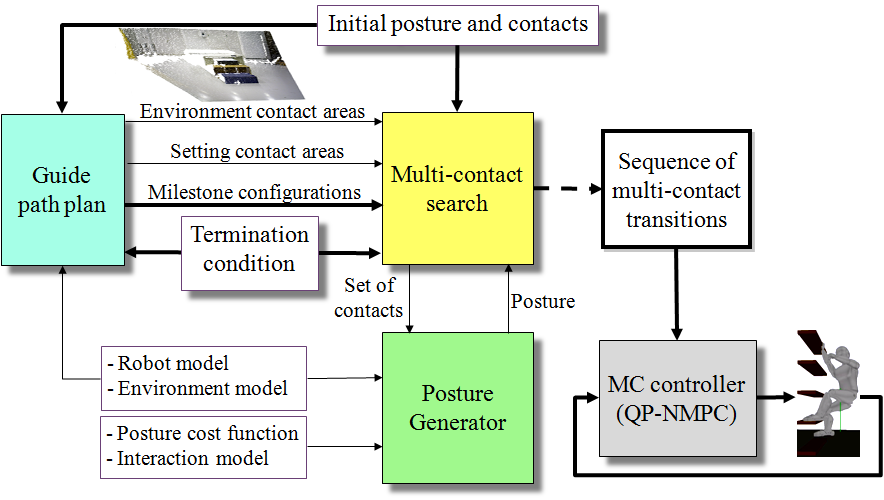
\includegraphics[width=\columnwidth]{papers/RAM2013/pictures/mcp.png}
 \caption{Multi-contact planner architecture.}
 \label{fig:mcp}
\end{figure}
The~\Figref{fig:mcp}{} illustrates the main components and their relation. The core of the planner consists in the multi-contact search and the posture generator. The former incrementally builds a tree of contact sets. The children of a node are obtained by adding or removing exactly one contact to its set. At each iteration of the search, the best leaf, according to a potential field, is expanded this way. The tentative sets of contacts are tested by the posture generator: for a given set of contacts, it attempts to find a configuration of the robot that satisfies these contacts while being statically stable, avoiding collision and staying within the robot's state and torques limits. This is done by automatically writing and solving a non-linear optimization problem. Upon success, the contact set is validated, and a new leaf is created. The goal is written as a set of constraints defining a sub-manifold of the configuration space. A node is the final node if its associated posture generation problem augmented by these constraints remains feasible. By backtracking from this final node to the initial root node, we obtain a sequence of nodes and thus a sequence of contact sets, that can be executed on the robot by a whole-body controller. We developed such a controller based on a quadratic programming (QP) formulation~\cite{bouyarmane:iros:2011}.

The potential field is derived from a crude path, made of a few key postures, that does not take contacts into account. Such a path is either user-defined or can be the output of a first dedicated planner~\cite{bouyarmane:icra:2009}.

The MCP relies largely on the 3D geometric models of the environment and robotic agents. In our previous work~\cite{escande:ras:2013,bouyarmane:ar:2012}, the geometric models are provided by the user. The contact transition for the robot are planned off-line and later executed by the robot assuming exactness of the models and their relative positioning. We aim at extending our MCP to deal directly with real data acquired by the robot. Subsequently, we must deal with two kinds of situations:
\begin{enumerate}
	\item the models of the objects in the environment are known: in this case adapting the MCP consists mainly in dealing with recognition, model superposition and handling uncertainties. In brief, once model superposition is achieved, we can use the 3D model for MCP as in~\cite{escande:ras:2013,bouyarmane:ar:2012}, yet some adjustments are needed.  
	\item the models of the hurdles and the environment are not known (e.g. disaster or outdoor environments, for example related to the Fukushima disaster that inspired the DARPA Robotic Challenge), MCP is to be achieved in an ego-centric way with models built from the robot's embedded sensors. This paper deals with this case and we describe how the MCP is modified to achieve this goal. In a nutshell, we construct planar surfaces from the 3D point clouds data and feed them to the MCP.
\end{enumerate}

In robotics, the use of 3D-based vision for recognition and navigation in environment known or partially unknown has first been used on mobile robots, evolving in flat environment, for example by coupling it with a SLAM system~\cite{whitty:acra:2012}. Another approach consists in extracting the surfaces from the point cloud, and then link them to the known environment or simply consider them as obstacles to be avoided~\cite{poppinga:iros:2008}. Since working on raw point clouds is costly because of the high number of data points, this extraction has also been enhanced~\cite{biswas:icra:2012} in order to be run in real-time. This approach has been recently experimented on a humanoid robot in~\cite{maier:humanoids:2012}, that combines two methods: the surface extraction from a point cloud, and the voxel-based 3D decomposition of the environment~\cite{nakhaei:humanoids:2008}. Still, since the robot only navigates in a flat environment, and does not realize manipulation tasks, the surfaces extracted from the 3D point cloud are down projected to a 2D plan, on which are based the navigation and collision avoidance processes.

The use of humanoid robots allows to navigate in more complex environment, and recently, some work has been done to make a humanoid robot go down a ramp~\cite{lutz:iros:2012} or climb stairs~\cite{osswald:iros:2012}. Yet, those methods use laser-based vision rather than point-cloud-based vision, so as to have a precise analysis of a known environment.

In this work, we aim at enabling a robot to analyze and plan a motion into a 3D environment. Hence, we use the surface extraction of a point cloud to directly have a global picture of the environment and determine the convex planar surfaces that the robot can use at its advantage to progress using the MCP. In our approach to make such an extension, we intentionally seek for technical solutions that minimize changes to be done on our existing MCP software.

\section{Building an understandable environment for our planner}

Our first concern is to build an environment that our multi-contact planner is able to ``understand'' and that can be extracted from a point cloud scene. 
%The simplest kind of entity that our planner would be able to deal with is an oriented rectangular plan surface. Though, it is clear that the real world cannot be precisely described by such things, so we add another level of detail to our world description by using convex polygonal planar surfaces. Therefore, starting from an acquired point cloud, we try to extract a relevant set of such geometrical entities that will be our first description of the surroundings of the robot. 

The simplest entity that our planner would be able to deal with and that could correctly describe the robot's environment is a set of convex polygonal planar surfaces. Therefore, starting from an acquired point cloud, we try to extract a relevant set of such geometrical entities that will be a first description of the surroundings of the robot.

In this section, we present the different steps we follow to create a set of relevant convex polygonal plane surfaces out of an acquired point cloud.
%\begin{itemize}
%\item Acquisition of the point cloud from a RGB and Depth sensor (see section~\ref{subsect:Acquisition})
%\item Filtering the point cloud(see section~\ref{subsect:Filtering})
%\item Plan extraction (see section~\ref{subsect:PlanExtract})
%\item Region growing segmentation(see section~\ref{subsect:region})
%\item Planar projection and hull convex generation (see section~\ref{subsect:PlanProjection})
%\item Re-orientation and transfer to the planner (see section~\ref{subsect:reorient})
%\end{itemize}

The~\Figref{fig:pipeline}{} illustrates the major steps of this point cloud treatment. We use Willow Garage's Point Cloud Library\footnote{\url{http://pointclouds.org/}} (PCL)~\cite{rusu:icra:2011} extensively for processing the point cloud.
\begin{figure*}[!htb]
	  \centering
	    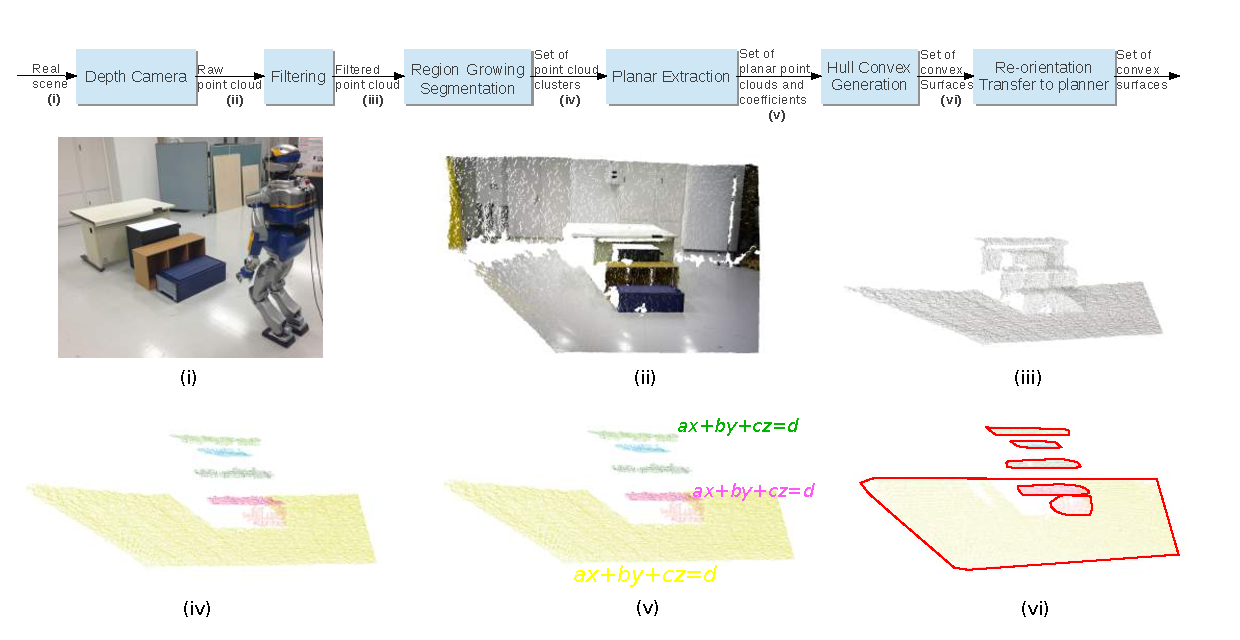
\includegraphics[width=\linewidth]{papers/RAM2013/pictures/complete_pipeline.pdf}
	    \caption{Top: flowchart describing the main elements of our algorithm and the type of data that is passed between them.\newline
	    \hspace*{27pt} Bottom: the data throughout the process, illustrated in the case of our first experiment (see Sec.~\ref{sec:plan1}).}
	    \label{fig:pipeline}
\end{figure*}


\subsection{Acquisition of point cloud from a RGB and depth sensor}
\label{subsect:Acquisition}

For our experiments, we use an Asus Xtion Pro camera, that provides a $640 \times 480$ pixel depth image, and the OpenNI Grabber. The obtained point cloud representing our scene contains points defined by their space coordinates and colors, and will be the entry of our point cloud treatment algorithm. We do not use the color information for now except for display purpose. It may however be useful in the future in matching object models with sensor data and to perform color-based region growing algorithms.

%\subsection{Parsing the .pcd file}
%
%This "initialization" step of our algorithm is staightforward; PCL implements some method to create a PointCloud object's
%instance directly out of a .pcd file.

\subsection{Filtering}
\label{subsect:Filtering}

In order to reduce the computation time and improve the efficiency of our point cloud treatment algorithm, it is necessary to reduce the overall size of the data set. We first remove all points further than 5 meters from the camera: such points are not reliable enough and thus a potential source of error for the following steps.
%We know that the data extracted from the Asus Xtion live camera are reliable only for points that are less than 5 meters away from it. Therefore, we eliminate all the 
%points that are further than that, since they would only be a source of error and wouldn't carry any valuable information.

We then downsample the cloud, since it is excessively dense for our purpose. To do so, we use a voxelized grid approach (using the {\tt pcl::VoxelGrid} class): we create a 3D voxel grid over the input point cloud data. Each voxel represents a group of points that are close enough from each other to be represented by a single point that would be their centroid. The centroid is chosen instead of the center of the voxel because it represents the real environment more accurately. Another advantage of this method is that the filter can easily be parametrized by choosing the size of the voxels. Those two steps allow us to greatly reduce the number of points in the data set. Typically, in our experiments, this divides the number of points by a factor 5 to 6.

\subsection{Region growing segmentation}
\label{subsect:region}

In order to divide a global point cloud scene into several sets of points that belong to the same flat area, we use a region growing algorithm~\cite{poppinga:iros:2008} (implemented in {\tt pcl::RegionGrowing} class). Its purpose is to merge the neighboring points that are close enough in terms of smoothness constraint. The output of this algorithm is a set of clusters representing sets of points that are considered to be a part of the same plane surface. This method is based on the comparison of the angles between the points' normals. 
%\note{\sout{This algorithm fits perfectly our needs, because it provides us with a list of sub-clouds (clusters), and each of those represents a flat area of the scene.}}
It is used right before the planar extraction algorithm in order to obtain an accurate list of points and plane models they represent. 

\subsection{Planar extraction}
\label{subsect:PlanExtract}

We use a plane segmentation to extract and group all the points that support a same plane model. Thus, we obtain a set of distinct point clouds. Indeed, this method finds the plane model that can carry the biggest set of points without regard for their proximity to each other. Then this first set of points is extracted from the initial point cloud and the algorithm can be applied to the remaining cloud recursively until the remaining cloud is small enough (in terms of number of points). For this purpose, we use the {\tt pcl::SACSegmentation} class.

This process works better on mostly flat point clouds (composed of a small number of large plane surfaces). Indeed, if it is applied to a point cloud that represents some stairs, instead of finding a set of points and a plane model for each step, it will most likely find a set of points and a plane model that represent the average slope of the stairs, and the reason for that is that the criteria of choice of a plane model is the greater number of points it bears, no importance is given to the proximity between the points of a planar set. That is why we apply the region growing algorithm~\ref{subsect:region}, that provides a list of clusters that represent the flat surfaces of the scene, before applying the planar extraction process on each of those clusters. 
It then computes a correct set of points and a plane model per region cluster.

\subsection{Planar projection and hull convex generation}
\label{subsect:PlanProjection}

The exact knowledge of all the data points contained in the plane model of a flat area is not necessary for our planning; we can reduce the point cloud to its convex hull without loss of information (except if the surface is concave, but this issue will be tackled in future works). In order to obtain the convex hull of each set of points, we first project every point of the set on its plane model ({\tt pcl::ProjectInliers} class) and then compute the 2D convex hull of the projected set of points ({\tt pcl::ConvexHull} class). After this step, each plane surface of the scene is represented by a frame composed of 3 vectors that are respectively a tangent, bi-tangent and normal vector of the plane model, an origin point that is the barycentre of the set of points and a small set of points that define its convex hull (the points' coordinates being calculated in the referential defined by the frame and the origin of the surface in order to make further calculations easier).

\subsection{Re-orientation and transfer to the planner}
\label{subsect:reorient}

Before sending the previously computed data to the planner, it is necessary to take into account the initial orientation of the camera. Indeed, if the camera was not aiming in a perfectly horizontal direction, then the entire point cloud would be misoriented. Therefore, it is necessary to re-orientate the surfaces before sending them to the planner. To do so, we simply apply a rotation matrix (that is computed from the initial camera orientation) to each of our data set's frame and origin to settle that problem. From there, the transfer of the surfaces to the planner can be done without any specific issue.

Re-orientation is done as a last step for the sake of performance: obviously we need to re-orient only a few frames, compared to an early re-orientation of the point cloud that would require to apply a transformation on thousands of points.

\section{Planning on point clouds}
\subsection{Convex surfaces inclusions}
We adjusted slightly our planner and posture generator to handle contacts between convex polygonal plane surfaces. The main modification made in the posture generator deals with properly writing the constraints that enforce the inclusion of one surface into another one. In our previous implementation, contacts are searched between rectangular patches attached to the robot body or the environment. Now any polygonal convex-shaped patch can be checked for inclusion in another; that is to say, the vertices of a convex 2D polygon are indexed counter-clockwise around its carrying plane surface's normal vector. A point that is inside the polygon is on the left side of all its edges. On the opposite, a point that is outside of the polygon will be on the right side of at least one of the polygon's edges. The following is the algorithm we use for the constraint generation:
\begin {algorithm}
\caption{Surface inclusion constraints for $S_i \subset S_j$}
\label{alg1}
\begin{algorithmic}
\STATE {Let $S_i$ and $S_j$ be two coplanar plane surfaces}
\STATE {$S_i = {p_0, p_1, \ldots, p_n}$ and $S_j = {q_0, q_1, \ldots, q_m}$}
\STATE {$\vec{N}$ is $S_i$'s normal vector}
\FOR{$k = 0 \to n$}
\FOR{$l = 0 \to m$}
\STATE { Constraint $: \left[\overrightarrow{q_lp_k}\times\overrightarrow{q_lq_{l+1}}\right].\vec{N} \leq 0$}
\ENDFOR
\ENDFOR
\end{algorithmic}
\label{algo:constraints}
\end{algorithm}

For a couple of coplanar surfaces $S_i$, $S_j$ respectively represented by $n$ and $m$ points, we create $n \times m$ constraints to ensure that the former is included in the latter one.

Once the surfaces are defined, it is possible to choose which ones are suitable for the robot to make contact with. Although it is not a mandatory step, it allows to reduce the exploration during the planning phase by removing undesired or inappropriate pairs of robot/environment surfaces. For the time being, this is determined by heuristics that are defined depending on the situation. For example, if we want the robot to walk on various surfaces, only surfaces that have a normal vector closely aligned with the gravity field would be selected as potential candidates (so as to eliminate the walls and other surfaces on which the robot cannot walk). Similarly, only surfaces located at a certain height can be considered for hand contact, etc.

\subsection{Collision detection}

In order to generate a feasible plan, we need to ensure that the robot avoids collisions with its environment and with itself. To do so, we consider each surface generated by our point cloud treatment algorithm as a thin 3D body. Basically, we extrude each surface by few centimetres in the direction opposite to its normal (provided that this normal is pointing toward the outside of the real body) and create a convex hull surface using {\tt QHull}~\cite{qhull:ACM:1996}. The collision avoidance is then computed by using the {\tt GJK} algorithm implemented efficiently for several convex shapes in~\cite{benallegue:icra:2009}.


\section{Results} 

In order to illustrate our method, we present two experiments in which the HRP-2 robot is asked to move $2$m forward. In both scenarios, this results in climbing on a table (The first one is $0.71$m-high and the second one is $0.53$m-high) with the help of various surrounding objects. The knowledge about the environment and surrounding objects is obtained from a point cloud captured by an ASUS Pro Xtion camera in one single shot. The camera was placed at the height of the robot's head, see~\Figref{fig:pipeline}{}.

All the computations of the following experiments are performed on a single thread of an Intel(R) Core(TM) i7-3840QM CPU at 2.80GHz, with 16Go of RAM.

\subsection{Plan 1: irregular stairs}
\label{sec:plan1}


In this first experiment, the robot has to walk up some irregular stairs made of several random pieces of furniture to reach its goal. The filtered point cloud contained 60286 points, that were split into 6 plane surfaces. The whole cloud processing was done in $2.7$ s. The planner computations generates a path of 11 nodes, some of which are depicted in~\Figref{fig:table-climbing-simulation-stair}{}. We notice that the robot climbs the stairs one by one without ever putting its two feet on the same step and without any noticeable problem.
In total, 23 nodes were generated and the planning time was $98.4$ s.

\begin{figure*}[!htb]
	\centering
	\renewcommand{\arraystretch}{0.2}
	\begin{tabular}{l c r}
	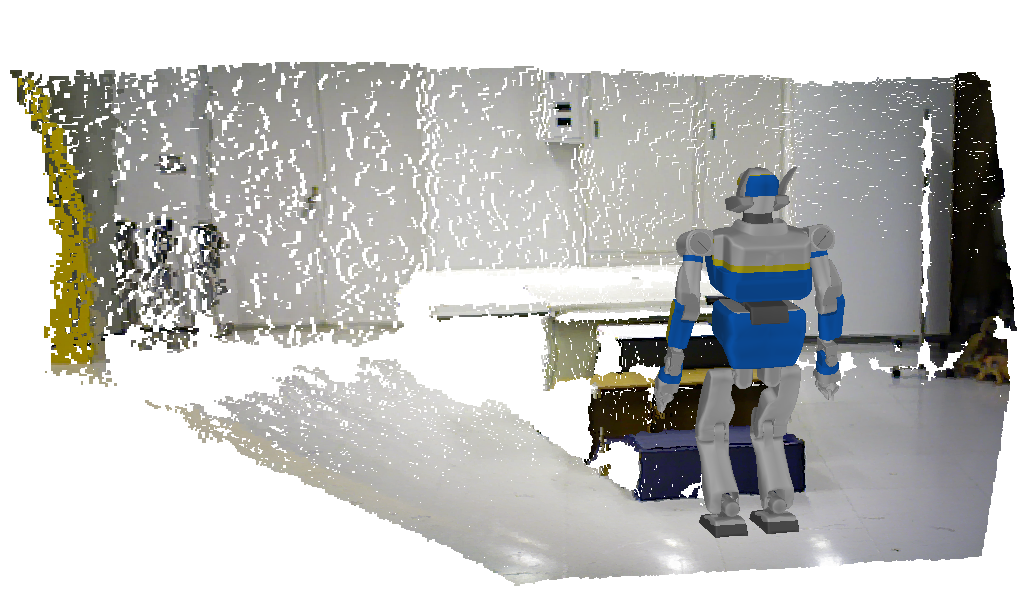
\includegraphics[width=.308\linewidth]{papers/RAM2013/pictures/Simu11Step0.png}&
	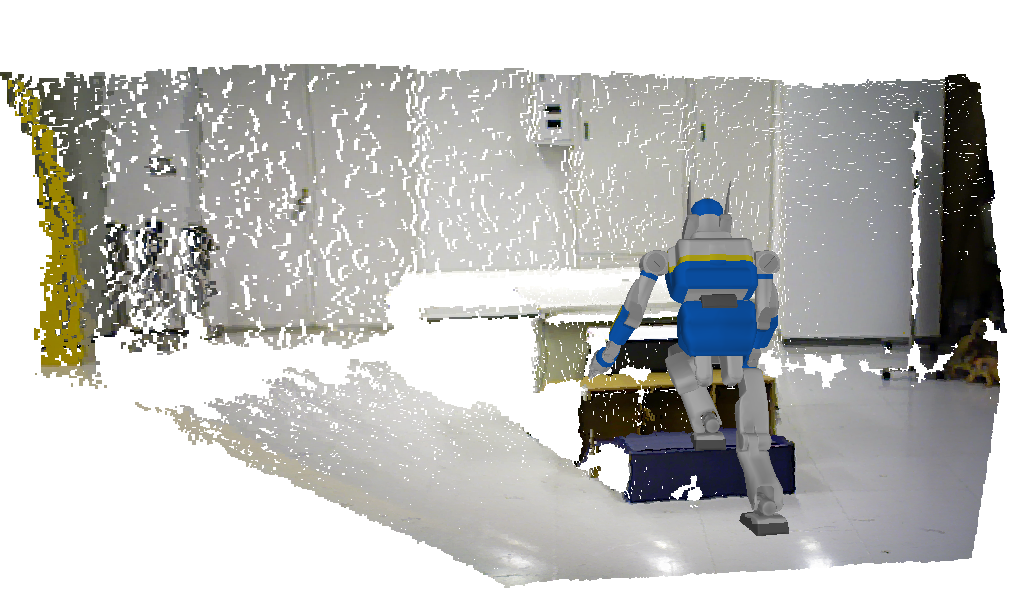
\includegraphics[width=.308\linewidth]{papers/RAM2013/pictures/Simu11Step3.png}&
	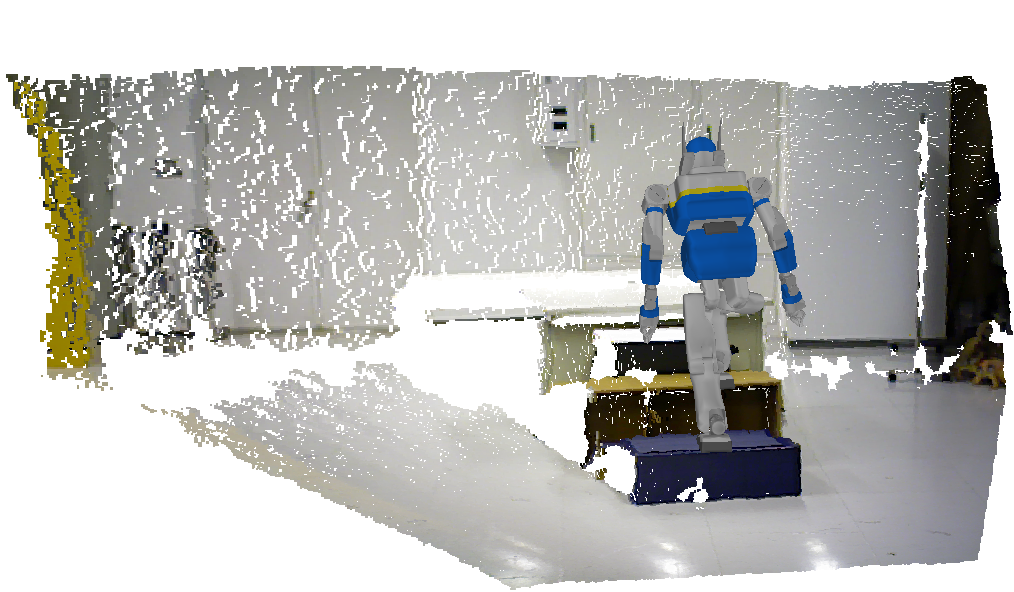
\includegraphics[width=.308\linewidth]{papers/RAM2013/pictures/Simu11Step5.png}\\
	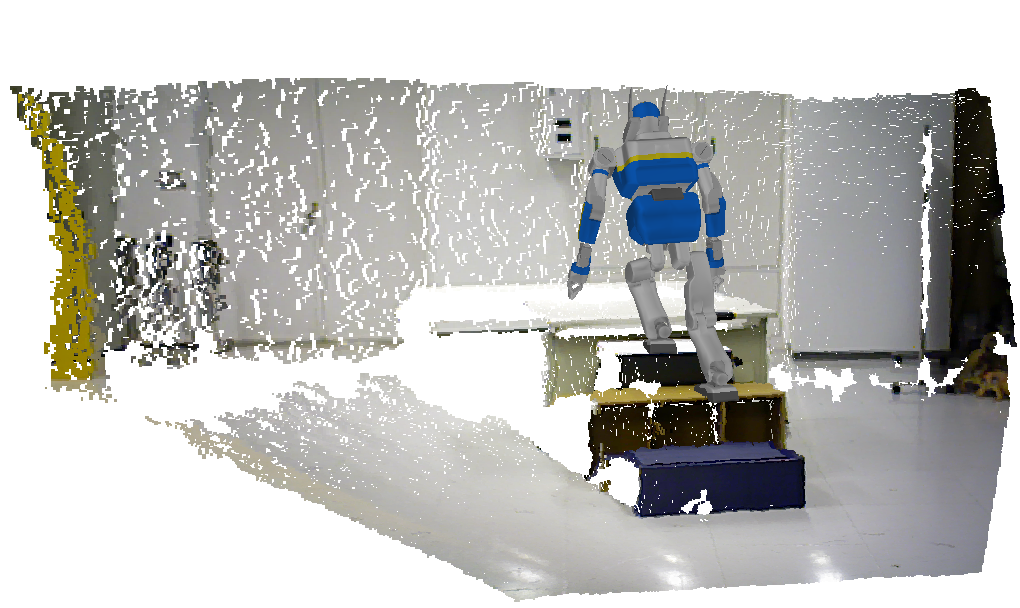
\includegraphics[width=.308\linewidth]{papers/RAM2013/pictures/Simu11Step7.png}&
	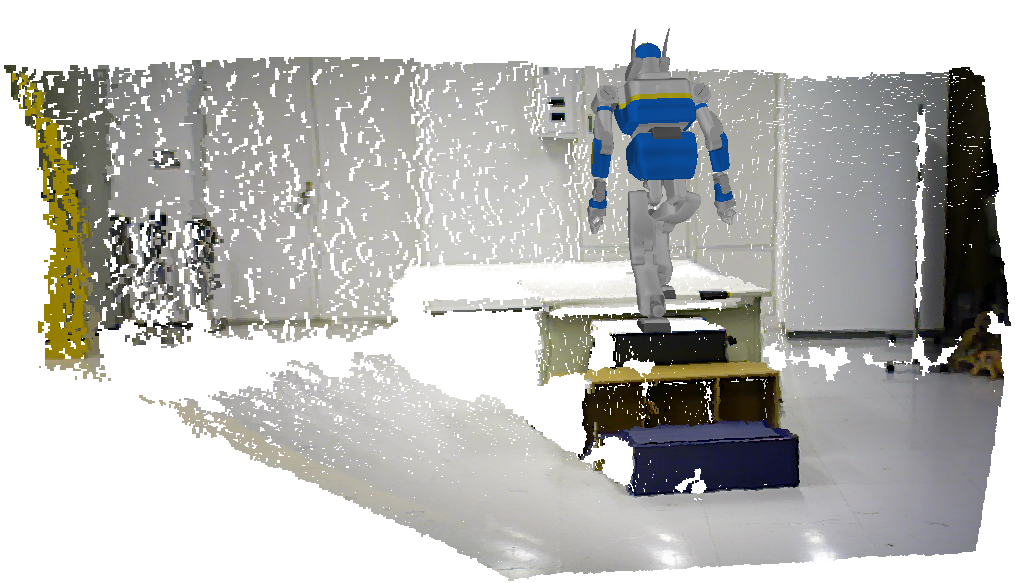
\includegraphics[width=.308\linewidth]{papers/RAM2013/pictures/Simu11Step9.png}&
	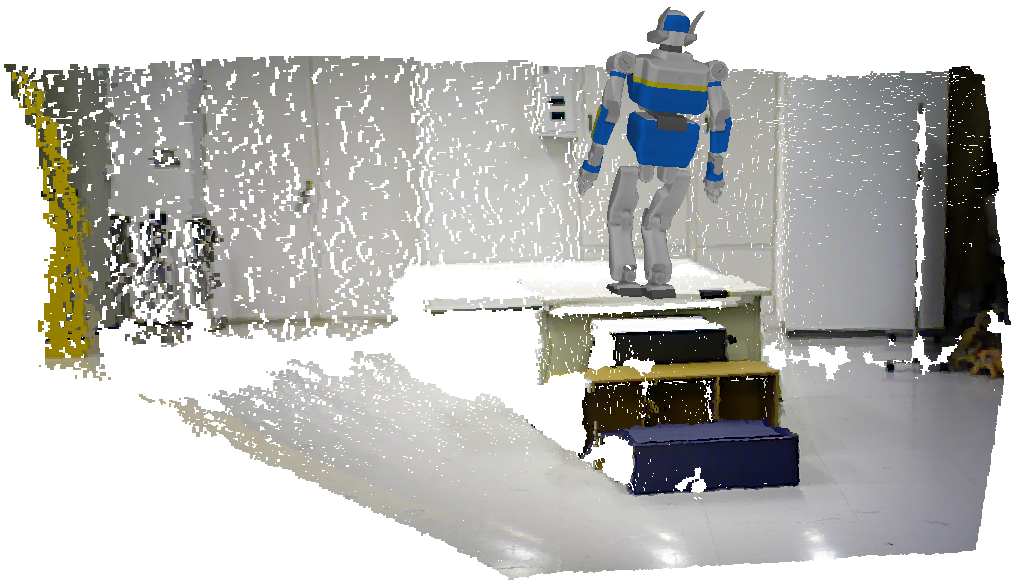
\includegraphics[width=.308\linewidth]{papers/RAM2013/pictures/Simu11Step10.png}\\
	\end{tabular}
	\caption{Table climbing simulation using irregular stairs. Of the 11 nodes of the path, we depicted the nodes 1, 4, 6, 8, 10 and 11.}
	\label{fig:table-climbing-simulation-stair}
\end{figure*}


\subsection{Plan 2: helping motion with the hand}
This second experiment was designed to showcase a more complex plan involving the use of the HRP-2 upper limbs. In this experiment, the filtered point cloud contained 66907 points, from which 11 surfaces were extracted. The whole cloud processing was done in $2.7$ s. The planner computation generates a path of 19 nodes, some of which are depicted in~\Figref{fig:crapahut-simulation}{}. To climb on the table, the robot uses its left arm and walks on an inclined slope before climbing a step at the end of the slope, once again, with the help of its left arm as support. In total, 40 nodes were generated and the planning time was $122.3$ s.

\begin{figure*}[!htb]
	\centering
	\renewcommand{\arraystretch}{0.2}
	\begin{tabular}{l c r}
		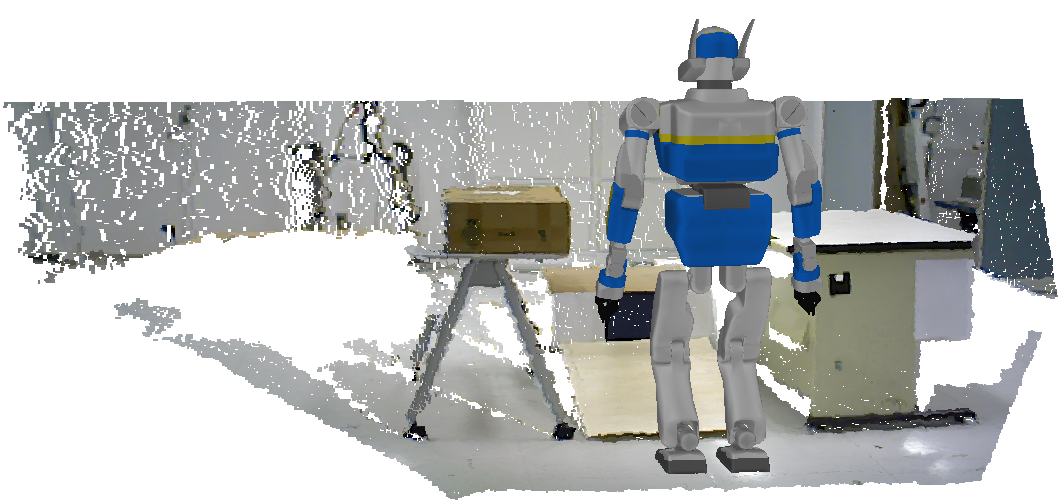
\includegraphics[width=.308\linewidth]{papers/RAM2013/pictures/Simu9Step0.png}&
		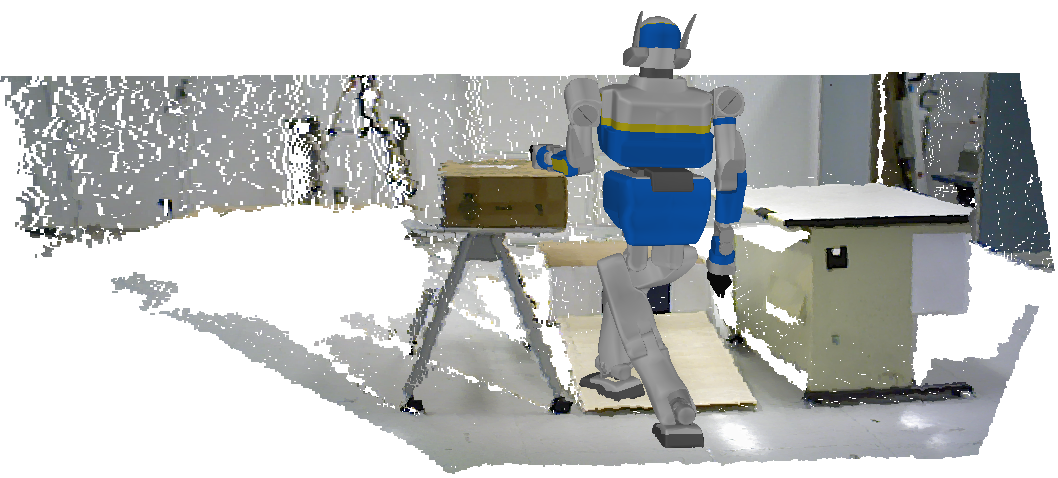
\includegraphics[width=.308\linewidth]{papers/RAM2013/pictures/Simu9Step6.png}&
		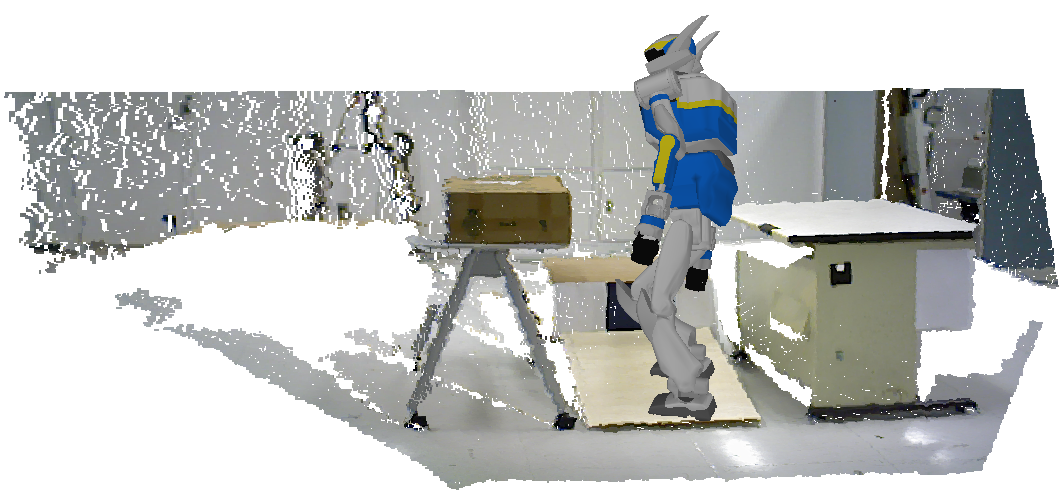
\includegraphics[width=.308\linewidth]{papers/RAM2013/pictures/Simu9Step11.png}\\
		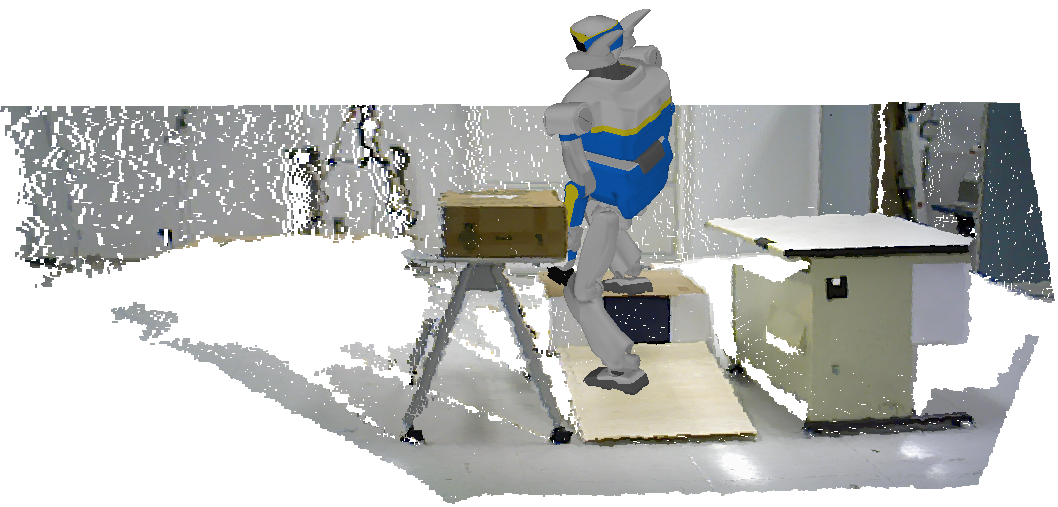
\includegraphics[width=.308\linewidth]{papers/RAM2013/pictures/Simu9Step14.png}&
		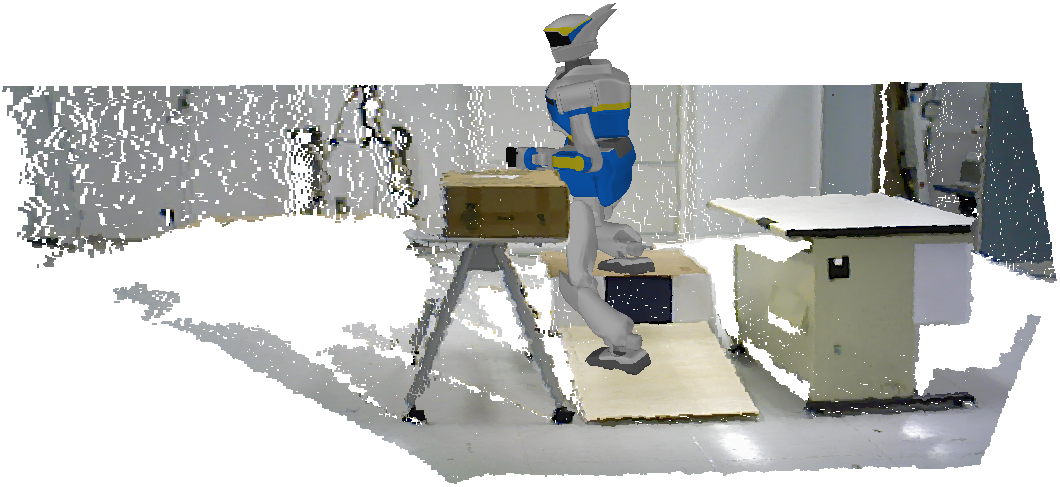
\includegraphics[width=.308\linewidth]{papers/RAM2013/pictures/Simu9Step16.png}&
		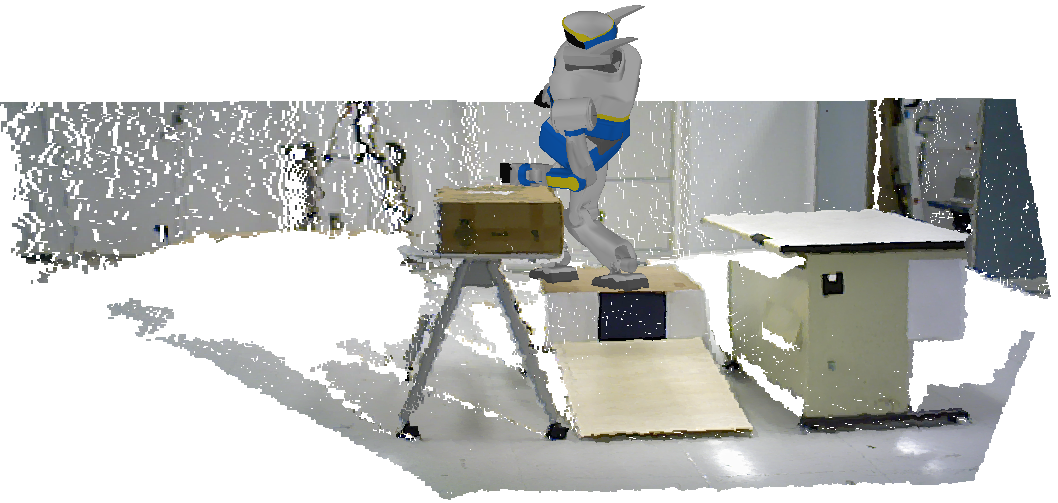
\includegraphics[width=.308\linewidth]{papers/RAM2013/pictures/Simu9Step17.png}\\
	\end{tabular}
	\caption{Slope and step climbing simulation. Of the 19 nodes of the path, we depicted the nodes 1, 7, 12, 15, 17 and 18.}
	\label{fig:crapahut-simulation}	
\end{figure*}


\section{Discussion}
This work is a first step toward a fully sensory-perception-based multi-contact planner. It raises several interesting questions on the way to adapt our MCP. 

One advantage of our approach is to avoid having to precisely position the robot in the environment prior to the plan execution. Yet, for now the positioning is done once and for all with the acquisition of the point cloud, before planning. When executing the plan, the robot might still deviate from it, for example a support might move, or a foot might contact a few centimetres away from where it was planned to, or the support might not be at its expected position because of measurement errors in the acquired point cloud. We thus need to close the loop between the planning and its execution. To do so, we need robust detection of discrepancies to be made by the robot. This can be achieved by combining point-cloud-based SLAM with contact sensing. Once the robot has acquired knowledge of its deviation or of the position error of the support, it has to adapt to it. This adaptation should not be time-consuming so as to not interrupt the execution for too long. A slight deviation can be recovered by simply positioning with care the next contacts and the closed-loop multi-contact controller shall work on guarded-motions basis. However, a bigger deviation might make the next contact stances infeasible. In this later case, re-planning the next contacts is necessary to go back to the plan. How many contacts have to be re-planned depends on the context. In difficult situations, changes in contacts might cascade up to requiring an entire re-planning. Recognizing the situation should be the task of a local planner that re-plans as few steps as possible. In case too much contacts must be reprocessed, the re-planning phase can be stopped before it ends and resumed at the next step.

This partial planning approach can also be seen in the context of semi-autonomous motion: an operator gives the overall direction with, for example, a joystick, and the planner reactively finds a sequence of a few contact sets to move as closely as possible in this desired direction. The operator is thus in charge of preventing the robot from getting stuck while the planner only concentrates on finding the correct contacts over a short time window.

Another question stems from the partial knowledge of the environment: it is not possible to give a guide path as we used to do with the 3D models. This guide path will necessarily be very crude, either a line to a desired position, or a plan in a known environment before it was changed (for example in the case of a disaster in a plant). The planning must then be driven also by the need of getting information about the environment, for example reaching a viewpoint allowing to see parts of the environment that were hidden before, filling empty spaces and possibly adding new supports on-the-fly. Planning is then only partial since necessary part of the environment might be unknown. 

Later on, the discovery of the environment might be improved by the use of other sensors. One can then imagine having the robot test for a contact to ensure a given surface is fit for support or that it is precisely at the position measured by vision. If the surface is not, this is another kind of discrepancy in the plan than needs to be handled by re-planning. 

\section{Conclusion}
We present preliminary results in extending our previous work in multi-contact planning to operate directly on environment that is built on-the-fly from a robot's embedded sensors. This first study makes use of depth camera and implemented modules from the PCL which extract planar surfaces that are fed to our MCP. We intentionally seek for technical implementations that minimize the changes on our existing MCP software and illustrate successful plans generated on the basis of 3D point clouds solely. 

The simulation results revealed that indeed our MCP does not require major adjustments to handle egocentric sensory data. Of course, this does not mean that we are fully satisfied since our results also suggest additional future work. 

First, although we choose to treat the case of not having 3D models, we believe that the implementation of an MCP with knowledge of the 3D model is necessary. For example, even in a disaster situations as in Fukushima nuclear power plants, the inside exploration videos available show that many objects kept their shape and were not totally destroyed (e.g. door, stairs, ladders, etc.). So having their model would then still permit our MCP to rely on 3D models to plan contacts for motion. PCL provides only partial information, it is then necessary to drive the planner by the mission objective and also a perceptual one (e.g. SLAM). Of course, our ultimate future plan is to handle uncertainties, control and planning recovery of discrepancies when they occur.

%\chapter{Integration of Non-Inclusive Contacts in Posture Generation}

\section{abstract}
In this paper we propose a simple way to formulate geometric contact formation to have an arbitrary intersection shape in a robotic (humanoid) posture generation problem. The contact shape is the outcome of our posture generator that is formulated as a non-linear optimization programming to fulfill a large variety of robot intrinsic limitations (e.g. joint and torque limits) and tasks (e.g. desired contact). Starting by defining convex areas of contact on the robot's body and the environment, that we call contact patches, we can generate contacts with arbitrary intersection of a pair of any of these predefined patches. Our geometric contact modeling writes very simply as additional constraints and variables added to the optimization problem, translating the search for an ellipse inscribed in the intersection of the pair of patches we want in contact. The result of our posture generator is then a configuration where contact patches are not necessarily included in one another. This allows our posture generator to propose contacts of different shapes with a non-predefined number of contact points (used later to compute reaction/contact forces). We illustrate the efficiency of our method in multi-contact posture generation with the HRP-2 and ATLAS humanoid robots with results that can not be generated automatically by existing methods.
%That is to say, the constraints formulating a new contact in the posture generator (that writes as a non-linear optimization problem), state that a surface is totally included into another. Moreover contact surfaces are modelled by four vertices only and are rectangular. This modelling has several limitations: (i) it excludes several viable solutions that the planar could exploit, (ii) it requires patching (by hand) the robot or the environment surfaces into somehow equivalent pieces of rectangles, (iii) do not allow singular contacts of type edge/plan (ladder) or rarely edge/edge and vertex/plan. The solution we provide solves this problem and extend our multi-contact planner possibilities to handle more complex scenarios without patching the robot or the environment surfaces and without limiting the number of contact points per surface of contact.


%%%%%%%%%%%%%%%%%%%%%%%%%%%%%%%%%%%%%%%%%%%%%%%%%%%%%%%%%%%%%%%%%%%%%%%%%%%%%%%%
\section{Introduction}
\label{sec:intro}

Generating viable robotic postures is a common problem encountered in sampling-based planning techniques and simulation of virtual characters. Generating desired initial, intermediary or finale posture configurations requires defining static task goals (e.g. reach a target point in 6D) to be done under intrinsic constraints such as joint limits, torque limits, avoiding non-desired self-collisions... and perceptual or extrinsic ones such as keeping an object in the embedded camera field-of-view, avoiding non-desired collisions with surrounding objects, etc. A common task objective assigned to virtual characters, avatars, or humanoid robots is to contact one or more of its links with the environment (e.g. feet touching the ground). Since our main applications target humanoid robots, we consider here posture generation problems inherent to these robots. However, the formalism applies to any kind of robots achieving contacts with its surroundings or itself.

Our problem is to generate multi-contact viable postures. As far as humanoids are concerned, we may add to the previously cited constraints, equilibrium and non-sliding. This paper is dedicated to the focused issue of how contact constraints can be written geometrically. Generating postures often uses state-of-the-art enhanced inverse kinematics or general-purpose non-linear optimization programming (where inverse kinematics can be seen as a particular solver case).  

%\begin{figure}
%\centering
%\begin{subfigure}{.5\columnwidth}
%  \centering
%  \setlength\fboxsep{0pt}
%  \setlength\fboxrule{1pt}
%  \fbox{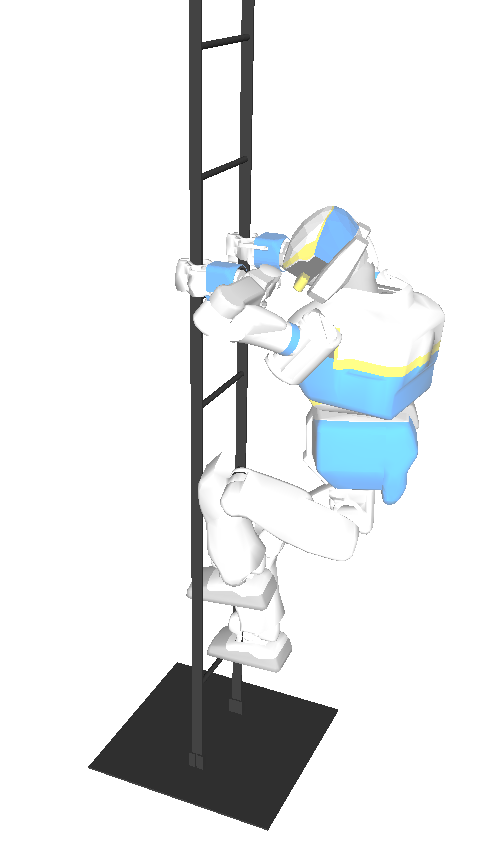
\includegraphics[width=\linewidth]{figure/hrp2_ladder_jrl.png}}
%  \label{fig:hrp2_jrl}
%\end{subfigure}%
%\begin{subfigure}{.5\columnwidth}
%  \centering
%  \setlength\fboxsep{0pt}
%  \setlength\fboxrule{1pt}
%  \fbox{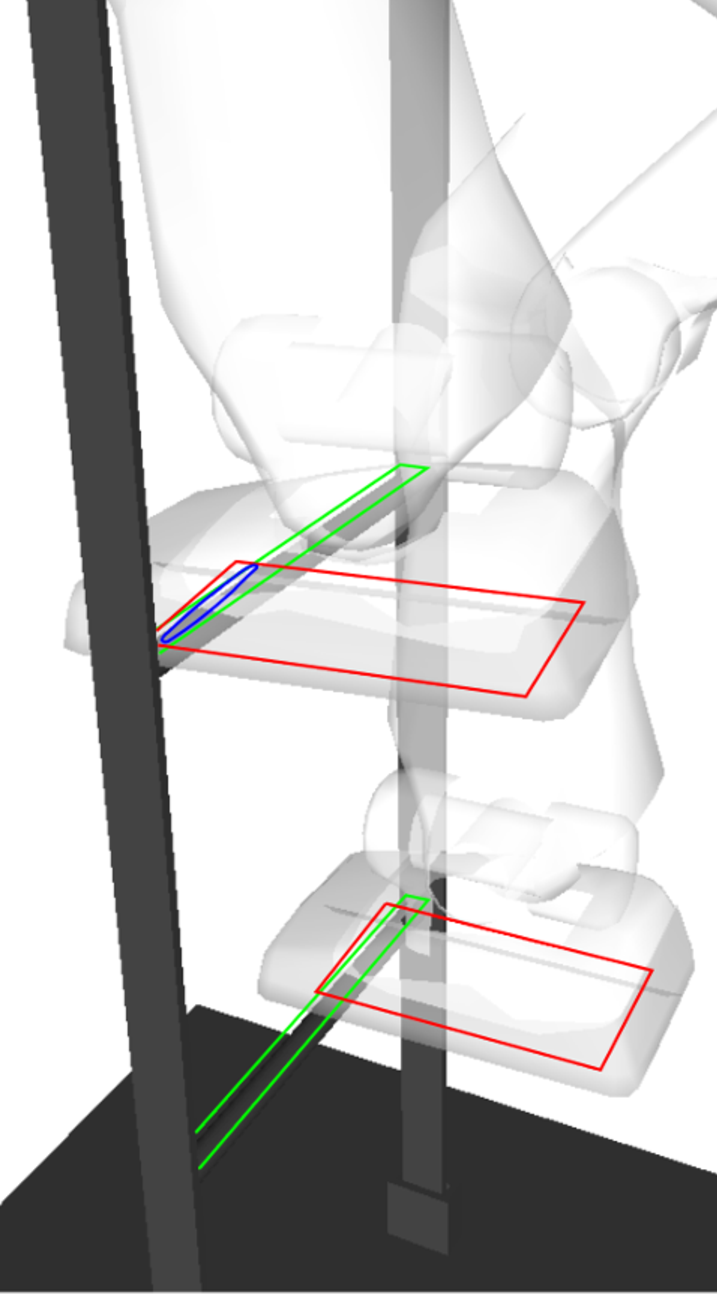
\includegraphics[width=\linewidth]{figure/hrp2_ladder_jrl_zoom.pdf}}
%  \label{fig:hrp2_jrl_zoom}
%\end{subfigure}
%\caption{Using non-inclusive contacts for ladder climbing\\(green/red: contact polygons; blue: contact ellipse)}
%\label{fig:hrp2_jrl_complete}
%\end{figure}  

\begin{figure}
\centering
  \centering
  \setlength\fboxsep{0pt}
  \setlength\fboxrule{1pt}
  \fbox{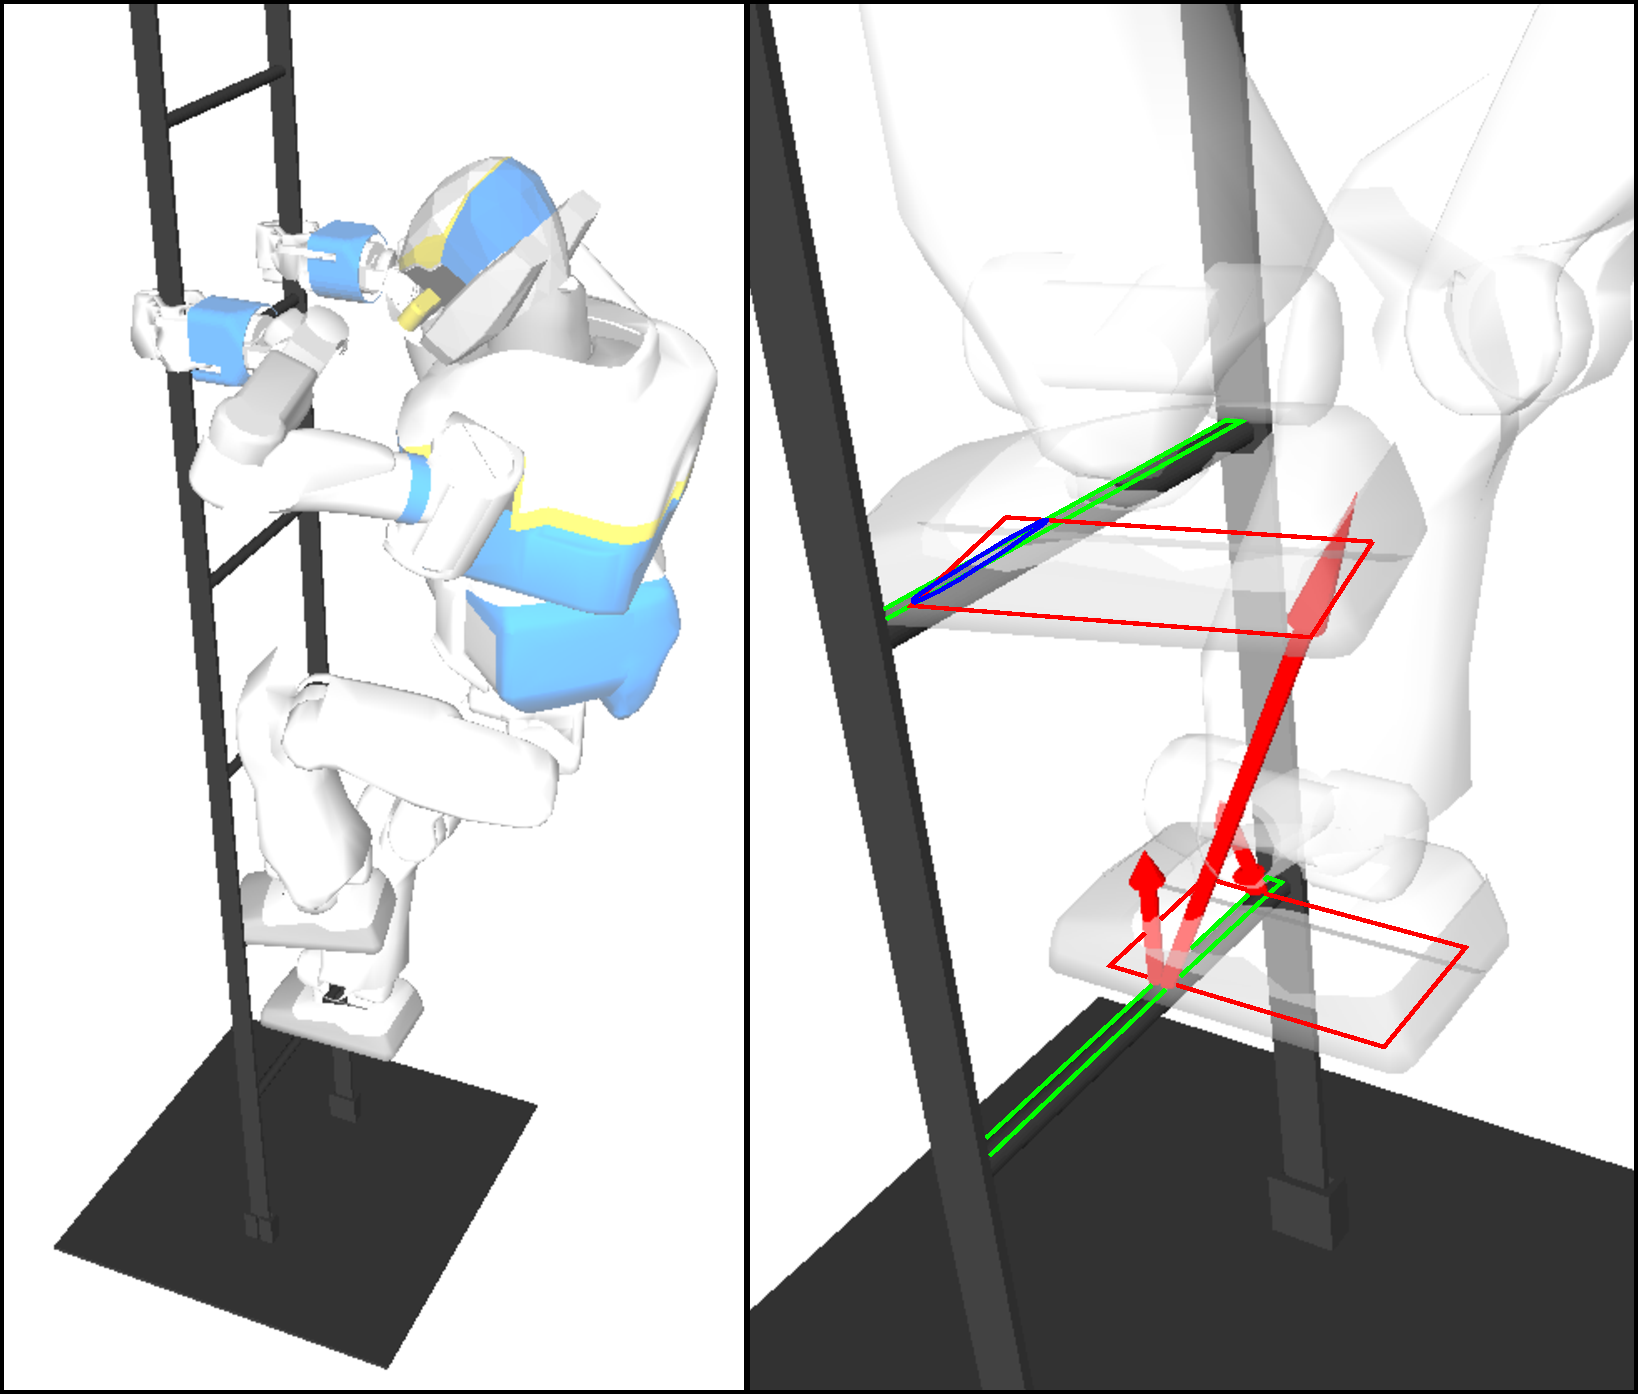
\includegraphics[width=.95\linewidth]{papers/IROS2014/figure/hrp2_ladder_jrl_5_combo.pdf}}
\caption{Using non-inclusive contacts for ladder climbing (green/red: contact polygons; blue: contact ellipse; red arrows: contact forces resultants)}
\label{fig:hrp2_jrl_complete}
\end{figure}  

In general, desired contacts write as hard constraints to fulfill in an optimization problem. Yet, we need to write the maths for, say, put the gripper on the wall and the left foot on the ground. In general, the maths of a gripper is a complex geometric description, so is often that of the environment. A contact is generally defined by a pair of points (one on each object in contact) and a pair of normal vectors. A hard contact constraint boils down to finding a posture in which the predefined authorized contact points and normal of each body match~\cite{zhang:TePRA:2013}\cite{hauser:IJRR:2008}. Likewise, in~\cite{osswald:iros:2011}, the position of the feet of the NAO robot is manually tuned in order to obtain statically stable position during the climbing of a spiral staircase. In~\cite{Chestnutt:2009:BNR:1733023.1733314}, the surface in contact is chosen according to two criteria: the position of the force sensors of the feet, and the type of contact desired. In~\cite{sentis:itro:2010}, the problem of contact discovery in not considered. In~\cite{mordatch:acm:2012}, two surfaces are considered in contact as soon as the center point of one of them touches the other one and their normals match. Although used in many papers, it is not difficult to see that this definition of contact excludes a series of possibilities that would have been obtained if the predefined points were placed in different configurations within their respective patches. Once the contact is established, one determines the intersection of contacting surfaces in order to find points on which reaction forces are to be computed. Several approaches require fixing the number of contact points or to have inclusive contact (i.e. one patch is fully included in the other)~\cite{bouyarmane:ar:2012}.

We provide a simple solution that relaxes hard contact constraints and gets rid of predefining the contact points by allowing them to travel within the patches. We consider that a contact is valid if the intersection between two distinct patches has an area greater than a given threshold. To enforce this, we require this intersection to contain an ellipse whose surface can possibly be maximized. Convex patches allow writing the inscription constraints easily by means of half-spaces. We finally implement our solution and present some examples for complex multi-contact posture generations with the HRP-2 and ATLAS robots, as shown in~\Figref{fig:hrp2_jrl_complete}. 


\section{Contact geometry formulation}

For our formulation, we consider a situation where a set of contacts between the robot and its environment are already made, and therefore fixed, and we want to add a new contact to this set. This doesn't induce any loss of generality since it just comes down to adding the contacts one by one.
To ensure that the new contact can be reached in a quasi-static way, we look for a configuration where the new contact is ``barely" made: the position of contact is reached, but that contact does not support any contact forces (this is a necessary step to generate a sequence of quasi-static transitions). We call it a geometric contact. Let us consider that the contact to add is defined by two flat surfaces $S_1$ and $S_2$ which are respectively delimited by two convex polygons $P_1$ and $P_2$. For this contact to be valid, it is obviously necessary that the intersection $P_1 \cap P_2$ is not empty. We propose a method in which the size of the contact area is approximated by the size of an ellipse that is inscribed in it. If such an ellipse is found and is of a sufficient size, then the contact is valid. This allows to consider contacts between surfaces that do not necessarily include each other.

An important remark is that the number of sides of the intersection polygon is not known a priori and, as shown on~\Figref{fig:polygon-inter}{}, this number can change depending on the configuration. Each time this number changes, the gradient of the area of the intersection is discontinuous. This is an issue for integrating any constraint or objective based on the area because we use a solver for smooth optimization problems. This issue could be dealt with by using non-smooth optimization routines, but such algorithms are slower and less available, and our posture generator is not designed to use them.
\begin{figure}[!htb]
 \centering
 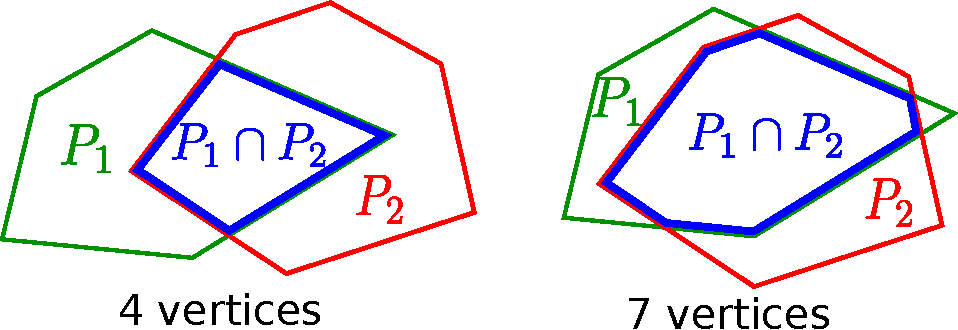
\includegraphics[width=0.8\columnwidth]{papers/IROS2014/figure/polygon-inter.pdf}
 \caption{Topological instability of $P_1 \cap P_2$}
 \label{fig:polygon-inter}
\end{figure}
Moreover, supposing that we want to write constraints based on the sides of the contact area, then, the number of constraints would change with the number of vertex of $P_1 \cap P_2$. The large majority of the optimization softwares cannot deal with a non-constant number of constraints. The solution proposed in section~\ref{sec:ellipse} overcomes these issues by defining a set of constraints that is independent from the topology of the intersection area.

\section{Posture generation}
\label{sec:pg}

The posture generation process aims at finding a posture that satisfies a set of tasks $\left\{ \mathcal{T}_i \right\}$ and that minimizes a cost function $\mbox{\emph{Cost}}$ by solving the following problem:
\begin{align}
\min_{\bf q, \bf f, \tau} & \quad \mbox{\emph{Cost}}({\bf q,f,\tau}) \nonumber\\
\text{s.t.}&
\left\{
\begin{array}{lr}
q_i^- \le q_i \le q_i^+\ \ \forall i=1,...,n \\
\tau_i^- \le \tau_i \le \tau_i^+\ \ \forall i=1,...,n \\
\epsilon_{ij} \le d(r_i({\bf q}), r_j({\bf q})),\ \ \forall(i,j)\in\mathcal{I}_{auto} \\
\epsilon_{ik} \le d(r_i({\bf q}, O_k)),\ \ \forall(i,k)\in\mathcal{I}_{coll}\\
\tau + J({\bf q})^T{\bf f} = {\bf g(q)}\\
s({\bf q,f})\le 0,\\
g_i({\bf q,f,\tau}) = 0\ \ \forall\mathcal{T}_i,\\
h_i({\bf q,f,\tau}) \le 0\ \ \forall\mathcal{T}_i.
\end{array}\right.
\label{eq:PG}
\end{align}
where the optimization variables $\bf q$, $\bf f$ and $\tau$ stand for the configuration, contact forces and joint torques of the robot.
Those constraints are illustrated in~\Figref{fig:PG}{} and are, in order of appearance:
\begin{itemize}
\item Joint limits
\item Torque limits
\item Auto-collisions, with $d(X,Y)$ the signed distance between objects $X$ and $Y$ and $r_i(\bf q)$ is the i-th body of the robot at configuration $\bf q$. $\mathcal{I}_{auto}$ is the set of pairs of bodies to monitor.
\item Collisions with the environment, $O_k$ being the k-th object in the environment and $\mathcal{I}_{coll}$ the set of pairs to monitor
\item Equation of static stability, with $J$ the Jacobian matrix of all points where the contact forces are applied, and $\bf g$ the gravity term.
\item Stability constraints describing the friction cones
\item Equality constraints describing the task $\mathcal{T}_i$
\item Inequality constraints describing the task $\mathcal{T}_i$
\end{itemize}

\begin{figure}[!htb]
 \centering
 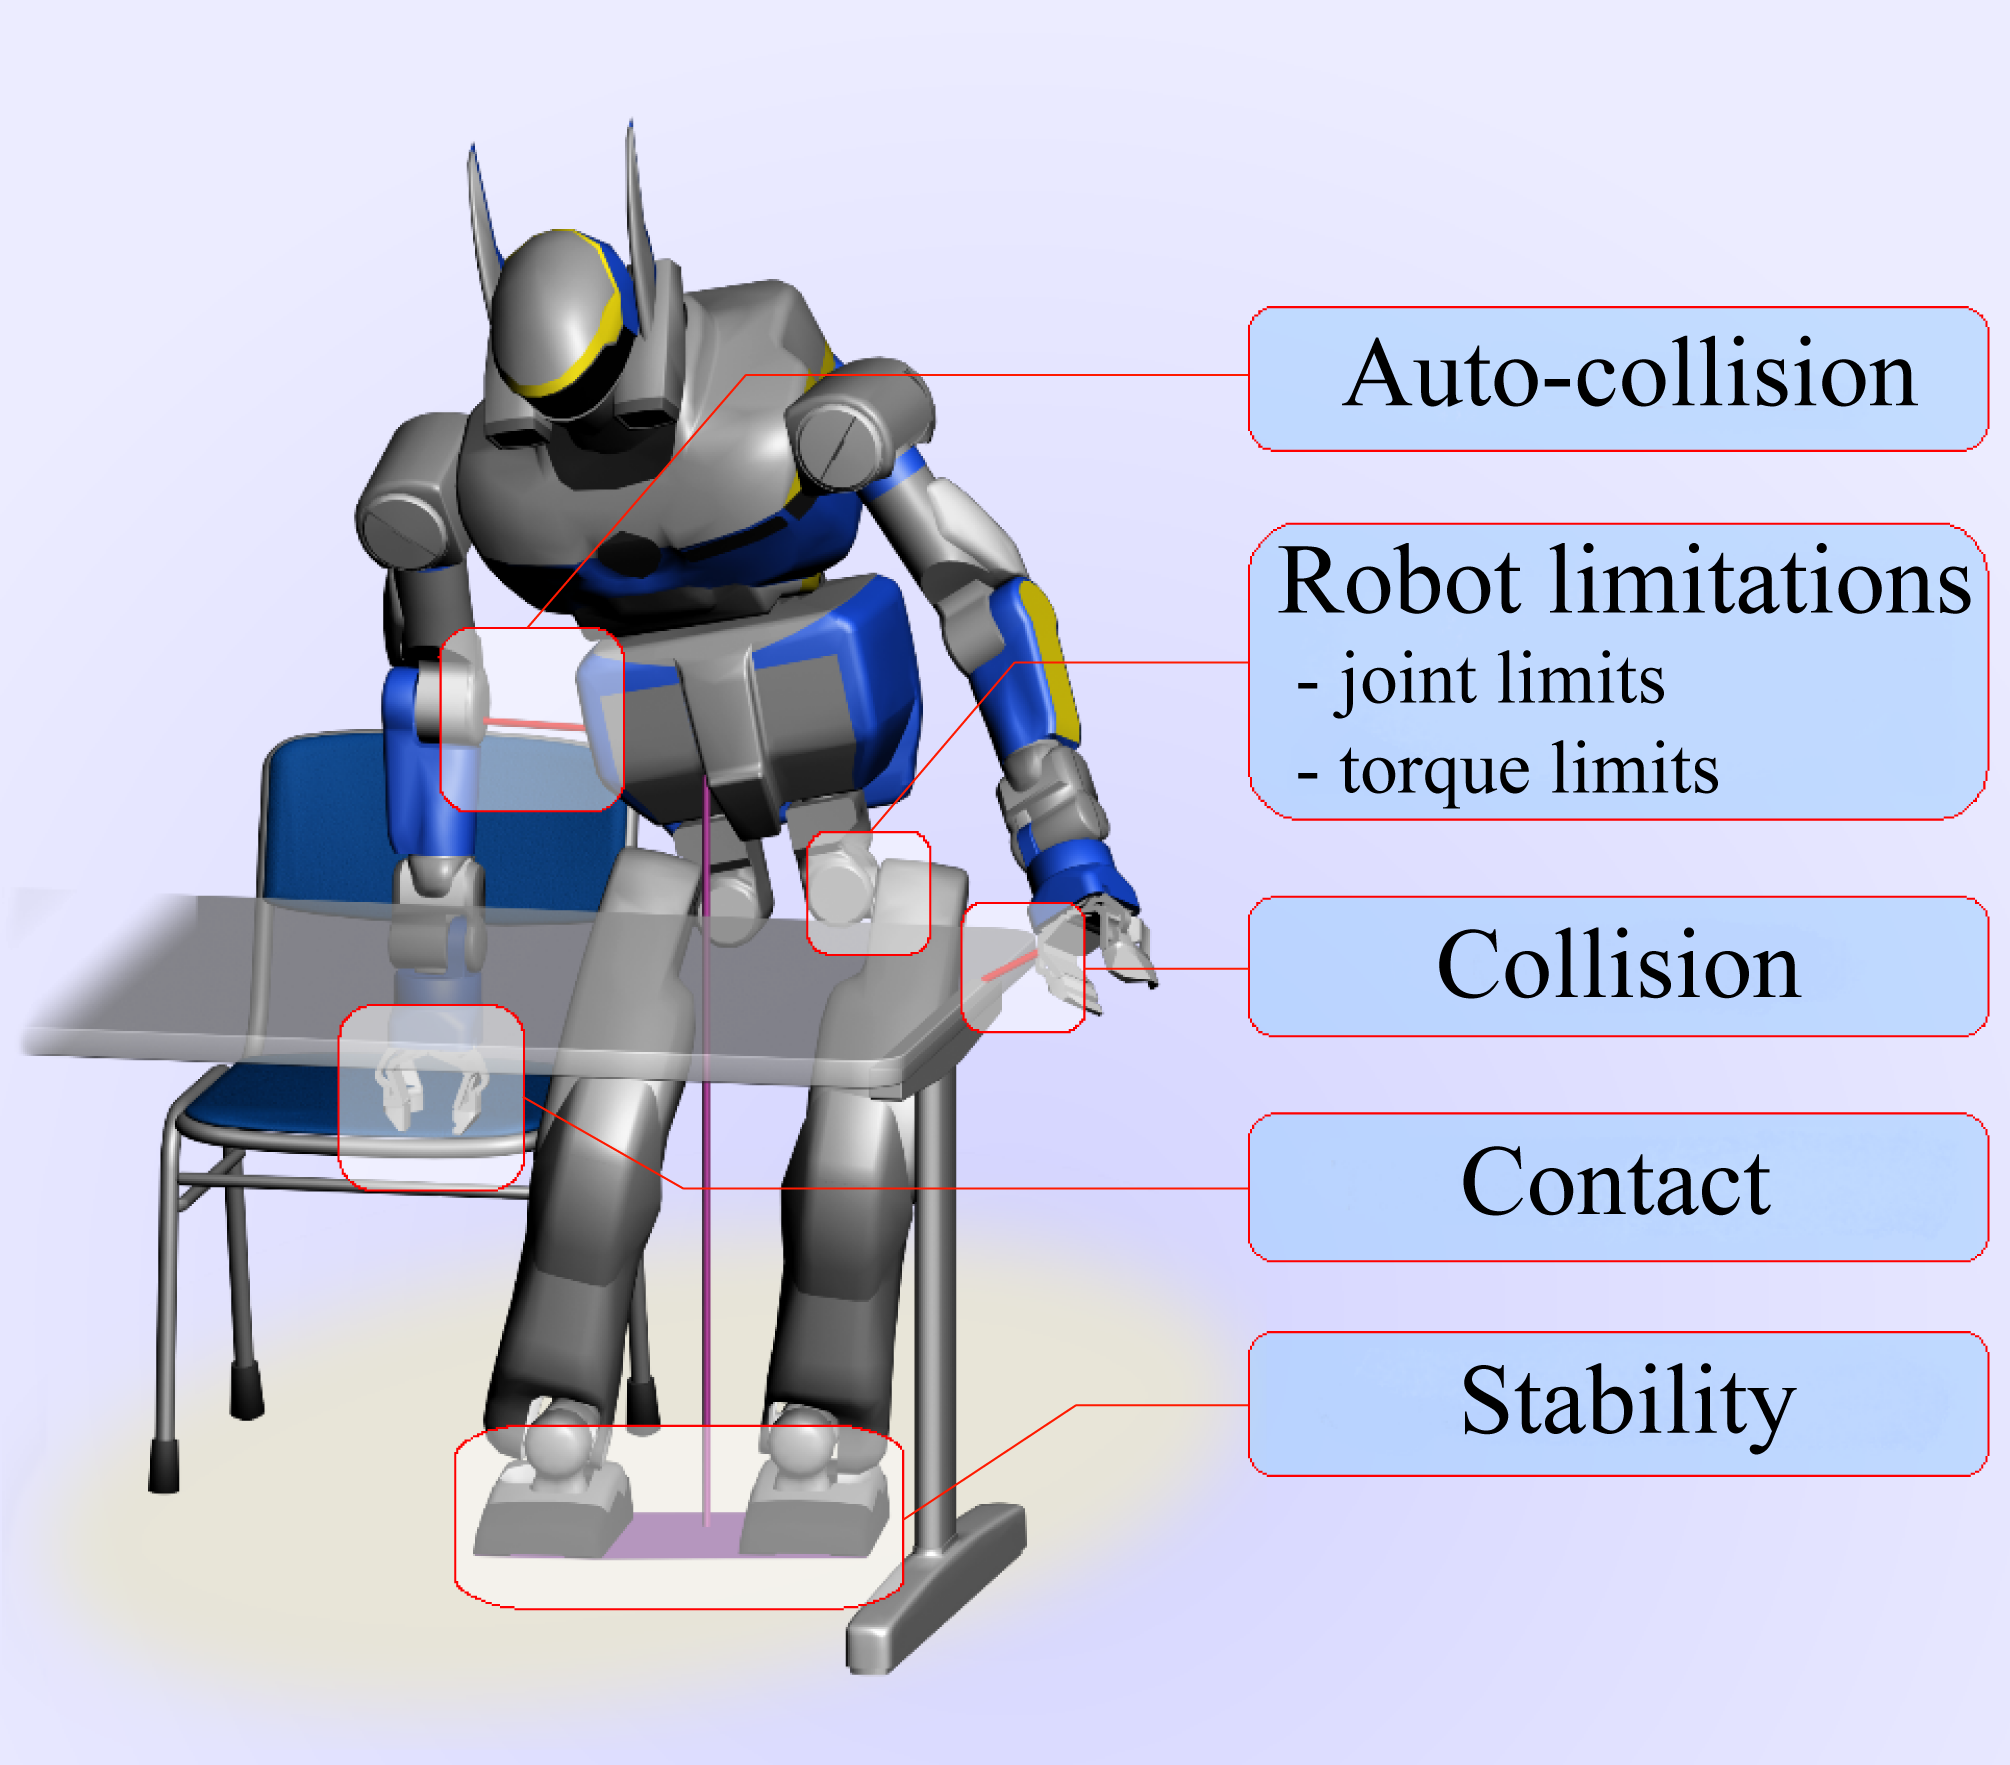
\includegraphics[width=.9\linewidth]{papers/IROS2014/figure/PG.png}
 \caption{Posture Generation's usual constraints}
 \label{fig:PG}
\end{figure}

A usual task $\mathcal{T}_i$ in the posture generation is to ensure that two surfaces are in contact. We consider 2 polygons $P_1$ and $P_2$ described in 2 frames $\mathcal{F}_1$ and $\mathcal{F}_2$, respectively. Each frame is defined by an origin point ${\bf O_i} = (o_i^x, o_i^y, o_i^z)$ and 3 orthogonal vectors $[{\bf T_i, B_i, N_i}]$. In those frames, the polygons are described as a set of $n_i$ bi-dimensional points $[p_i^0, p_i^1,\ldots, p_i^{n_i-1}]$ lying in the $[{\bf O_i, T_i, B_i}]$ plane.
To ensure the contact between those two surfaces, it is necessary that the planes defined by $[{\bf O_1, T_1, B_1}]$ and $[{\bf O_2, T_2, B_2}]$ are coplanar. This is expressed by the set of equations~(\ref{eq:coplanarity}). Those equations define a floating contact, where the co-planarity is ensured and the surfaces can translate along $\bf T_1$ and $\bf B_1$ and rotate around $\bf N_1$.
\begin{equation}
\left\{
\begin{array}{lr}
{\bf (O_2-O_1).N_1} = 0 \\
{\bf T_2.N_1} = 0 \\
{\bf B_2.N_1} = 0 \\
{\bf -N_2.N_1} \le 0
\end{array}
\right.
\label{eq:coplanarity}
\end{equation}

However, this is not sufficient since nothing ensures that the intersection of $P_1$ and $P_2$ is not empty.
Up to now, to avoid the problems described in section~\ref{sec:background}, we were requiring that one of the two polygons was completely included into the other (which restricted the contact configuration possibilities) or by defining a fixed contact position by hand, in which case the non-emptiness is ensured by the user. The next section presents a more general formulation
%The inclusion of the polygon $P_i$ in the polygon $P_j$ is imposed by making sure that each vertex of $P_i$ is on the left side of every edge of $P_j$, that is, assuming that both polyg polygonsons are described counter-clockwise around the ${\bf N}$ vector of the frame to which they are attached, the algorithm \ref{alg:inclusion} summarizes that constraint.
%\begin {algorithm}
%\caption{Surface inclusion constraints for $S_i \subset S_j$}
%\begin{algorithmic}
%\STATE {Let $S_i$ and $S_j$ be two coplanar plane surfaces}
%\STATE {$S_i = {p_0, p_1, \ldots, p_n}$ and $S_j = {q_0, q_1, \ldots, q_m}$}
%\STATE {$\vec{N}$ is $S_i$'s normal vector}
%\FOR{$k = 0 \to n$}
%\FOR{$l = 0 \to m$}
%\STATE { Constraint $: %\left[\overrightarrow{q_lp_k}\times\overrightarrow{q_lq_{l+1}}\right].\vec{N} \leq 0$}
%\ENDFOR
%\ENDFOR
%\end{algorithmic}
%\label{alg:inclusion}
%\end{algorithm}

\section{Non inclusive contact constraints}
\label{sec:ellipse}
\subsection{Main Idea}
\label{subsec:idea}
We present our main contribution: a smooth formulation of the non empty intersection between two contact surfaces. We assume that co-planarity of $S_1$ and $S_2$ is obtained by using the constraints presented in the previous section. Here we focus on the intersection of the two polygons $P_1$ and $P_2$, respectively describing the contours of $S_1$ and $S_2$.
As we pointed out earlier, a problem with computing the area of intersection of two polygons comes from the fact that depending on their positions in space, the number of edges of their intersection can change (cf.~\Figref{fig:polygon-inter}{}), which induces discontinuity of the gradient of the area and change of the number of constraints associated with this contact.

To avoid dealing with these changes of topology, we consider using an ellipse $\mathcal{E}$ included in $P_1 \cap P_2$ to estimate the area of the intersection. Since $P_1$ and $P_2$ are convex polygons, then $P_1 \cap P_2$ is also a convex polygon. A convex polygon can be seen as an intersection of half-planes based on the lines supporting its edges. Thus, an ellipse is inside a convex polygon if it lies entirely in the corresponding half-planes. Having the ellipse be included in the intersection of two polygons is equivalent to having it included in both polygons:
\begin{equation}
\mathcal{E} \subset P_1 \cap P_2 \ \Longleftrightarrow \ 
\mathcal{E} \subset P_1 \ \ \wedge \ \  \mathcal{E} \subset P_2
\end{equation}
Even if the number of edges of $P_1 \cap P_2$ can change, the numbers of edges of $P_1$ and $P_2$ respectively are fixed. 
%\begin{wrapfigure}{r}{0.4\columnwidth}
%  \begin{center}
%    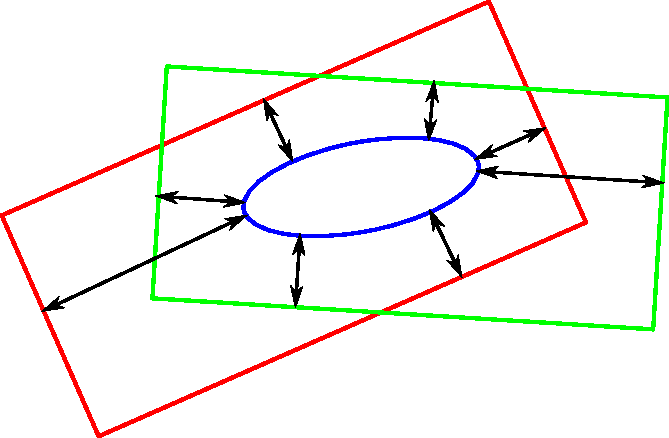
\includegraphics[width=0.4\columnwidth]{papers/IROS2014/figure/distance.pdf}
%    \caption{Distance ellipse-polygons}  
%  \end{center}
%  \label{fig:distance}
%\end{wrapfigure}
%Therefore, if we ensure that the ellipse $\mathcal{E}$ is on the left side of each segment defining $P_1$ and $P_2$, then it is inside $P_1 \cap P_2$. 
To assert that an ellipse lies in a half-plane, we need a function that is positive when the ellipse is in it (with zero value when the ellipse is on the edge) and negative if not. The signed distance to the line defining the half-space is a good candidate (distance ellipse-line if the ellipse is in the half-plane, opposite of the penetration distance if not), but actually, any pseudo-distance does the job. And a sufficient condition for the ellipse to be inside the polygons intersection is that the pseudo-distance between the ellipse and each edge of both polygons is positive (see~\Figref{fig:distance}{}). By considering each edge separately as opposed to the (pseudo-)distance of the ellipse to a whole polygon, we can write smooth constraints with a simple pseudo-distance function. We develop such a pseudo-distance in the next subsection. 
%In order to measure the fact that a point is on the left side of an oriented segment we use a signed distance $d_s$, this signed distance is positive and equal to a usual distance when the point is on the left side of the segment and is negative and equal to the opposite of the usual distance when the point is on the right side of the segment. 
% and algorithm~\ref{alg:ellipse-in-intersection} where $d_s$ stand for the pseudo-distance.
%\begin {algorithm}
%\caption{Inclusion of ellipse $\mathcal{E}$ in polygon intersection}
%\begin{algorithmic}
%\STATE {Let $P_1$ and $P_2$ be two coplanar convex polygons}
%\STATE {Let {\bf V} be an empty vector}
%\FORALL{Edge E in $P_1$}
%\STATE {Add $d_s(\mathcal{E}, E)$ to {\bf V}}
%\ENDFOR
%\FORALL{Edge E in $P_2$}
%\STATE {Add $d_s(\mathcal{E}, E)$ to {\bf V}}
%\ENDFOR
%\IF {{\bf V}$\succ 0$ (all terms of {\bf V} are positive)}
%\STATE {Return $\mathcal{E} \subset P_1 \cap P_2$}
%\ELSE
%\STATE {Return $\mathcal{E} \not\subset P_1 \cap P_2$}
%\ENDIF
%\end{algorithmic}
%\label{alg:ellipse-in-intersection}
%\end{algorithm}
%
\begin{figure}[!htb]
 \centering
 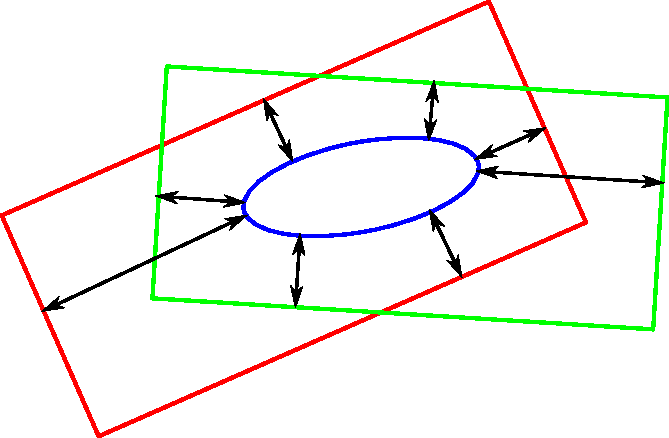
\includegraphics[width=0.4\columnwidth]{papers/IROS2014/figure/distance.pdf}
 \caption{Distance between $\mathcal{E}$ and $P_1 \cap P_2$}
 \label{fig:distance}
\end{figure}

\subsection{Pseudo-distance}
\label{subsec:formulation}
To estimate the constraint of inclusion of the ellipse $\mathcal{E}$ in both polygons $P_1$ and $P_2$, we need to compute the signed distance between $\mathcal{E}$ and each segment of the polygons. Computing the distance between an ellipse and a line is not straightforward, whereas the distance between a line and a circle is very easy to compute. Also, we note that in the frame $F_\mathcal{E}$ defined by the ellipse's axes and pseudo-radius, the ellipse is a circle of radius $r_{\mathcal{E}}=1$ (The x-unit along the first axis of the ellipse is $r_x$, the first radius of the ellipse, the y-unit along the second axis of the ellipse is $r_y$, the second radius). The transformation from the original frame $F_0$ in which the ellipse and the polygons are described to the ellipse's frame $F_\mathcal{E}$ is just the composition of a rotation and a scaling of the space along the axes of the ellipse with a scaling vector $[\frac{1}{r_x}, \frac{1}{r_y}]$. The effect of such a transformation applied to an ellipse and two polygons is shown in~\Figref{fig:pseudo-distance}{}. %Also, those transformations will not modify the validity of our constraint, indeed, the distance between $\mathcal{E}$ and any segment $E$, computed in $F_\mathcal{E}$, is a pseudo-distance in $F_0$. Therefore, we still get all the information needed to ensure the inclusion of $\mathcal{E}$ in $P_1 \cap P_2$.
We thus defined the following pseudo-distance from an ellipse to a half-plane as the signed Euclidean distance from the corresponding unit circle to the transformed half-plane in the frame $F_\mathcal{E}$.

\begin{figure}[!htb]
 \centering
 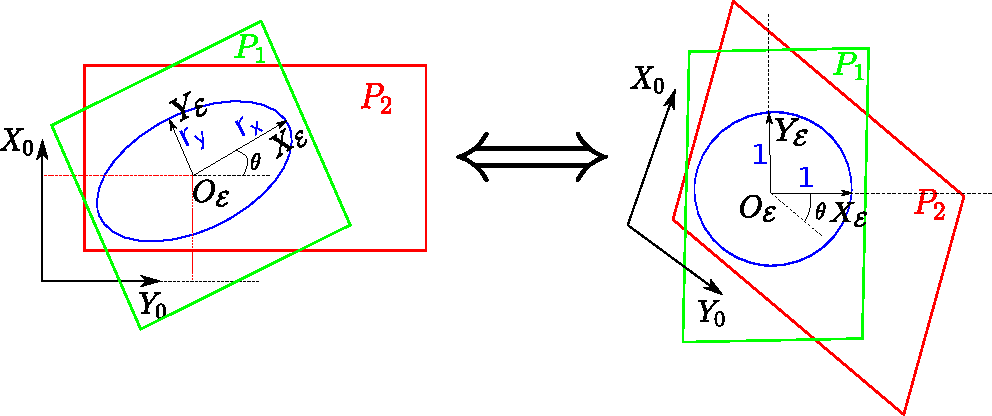
\includegraphics[width=\linewidth]{papers/IROS2014/figure/pseudo-distance.pdf}
 \caption{Transformation from $F_0(O_0, X_0, Y_0)$ to $F_\mathcal{E}(O_\mathcal{E},X_\mathcal{E},Y_\mathcal{E})$}
 \label{fig:pseudo-distance}
\end{figure}

Now let us consider a single segment $p_i p_j$ and an ellipse $\mathcal{E}$ defined in $F_0$.
The expression of a vector ${\bf v}_{F_0}^T = [v_x, v_y]_{F_0}$ in $F_\mathcal{E}$ is obtained by applying the formula~(\ref{eq:F0-to-FE})
\begin{equation}
{\bf v}_{F_\mathcal{E}} =
\begin{pmatrix}
\frac{1}{r_x} & 0 \\
0 & \frac{1}{r_y}
\end{pmatrix}
.\begin{pmatrix}
\cos(\theta) & \sin(\theta) \\
-\sin(\theta) & \cos(\theta)
\end{pmatrix}
.{\bf v}_{F_0}
\label{eq:F0-to-FE}
\end{equation}
In $F_\mathcal{E}$, the distance between the circumference of $\mathcal{E}$ and the segment $p_i p_j$ is: 
\begin{equation}
	d_s(\mathcal{E}, p_i p_j) = \frac{ \left(\overrightarrow{p_i p_j}\right)_{F_\mathcal{E}} \times \left(\overrightarrow{p_i O_\mathcal{E}}\right)_{F_\mathcal{E}}}{\| \overrightarrow{p_i p_j}\|_{F_\mathcal{E}}}-r_{\mathcal{E}}
\end{equation}
where $\times$ denotes the cross product and $O_{\mathcal{E}}$ is the center of the ellipse.

To avoid numerical problems when the segment $p_i p_j$ is small, (see sec.~\ref{subsec:singular cases}), it is preferable to multiply this distance by $\| \overrightarrow{p_i p_j}\|_{F_\mathcal{E}}$ before using it as a constraint. Then we get the following constraint: 
\begin{equation}
	-\left(\overrightarrow{p_i p_j}\right)_{F_\mathcal{E}} \times \left(\overrightarrow{p_i O_\mathcal{E}}\right)_{F_\mathcal{E}}+\| \overrightarrow{p_i p_j}\|_{F_\mathcal{E}} r_{\mathcal{E}} \leq 0
\label{eq:pseudo-distance}
\end{equation}

The combination of these equations~(\ref{eq:F0-to-FE}) and (\ref{eq:pseudo-distance}) applied for each edge of the polygons gives us all the necessary tools to develop a set of constraints that ensures that an ellipse is in the intersection of two polygons.


\subsection{Modification of the optimization problem}
To include the above idea in our posture generation, we need to modify the optimization problem~(\ref{eq:PG}) as follows.
Each non inclusive geometrical contact adds five variables to the optimization vector, corresponding to the position, orientation and radiuses of the ellipse ($x$, $y$, $\theta$, $r_x$ and $r_y$). One constraint of ellipse inclusion (as described above) is added to the problem for each edge of the polygons. The parameters $r_x$ and $r_y$ are given lower positive bounds to ensure that the ellipse is not empty. The existence of a contact between $S_1$ and $S_2$ is thus transformed into the existence of $r_x$ and $r_y$ respecting their bounds.
In summary, this kind of constraint adds 5 variables and $card(P_1)+card(P_2)$ constraints to the optimization problem, while the ``usual" inclusion constraint adds 0 variable and $card(P_1)card(P_2)$ constraints.
The existence of the contact can alternatively be enforced by imposing a minimum area for the ellipse.

\subsection{Maximization of the contact area}
\label{subsec:optim-ellipse-area}

%The previous section showed how to write a constraint describing the inclusion on any ellipse in the intersection of polygons. But it does not guarantee anything about the size of this ellipse nor about the size of the contact area. 
The formulation in the above section only ensures the existence of a contact of minimal size.
However, one could want to make sure to find a contact area as large as possible, so that it is more likely to be able to support strong forces and ensure strong friction forces, which is helpful to ensure the stability of the robot. Therefore, it seems appropriate to try and maximize the area of contact between two polygons. As explained before, computing the area of the intersection surface is not a good practice in our case. But we know that the ellipse computed as above gives a lower bound of the contact area.
\begin{equation}
\mathcal{E} \subset P_1 \cap P_2 \Longrightarrow  \mathcal{A}(\mathcal{E}) \le \mathcal{A}(P_1 \cap P_2)
\end{equation}
with $\mathcal{A}(X)$ being the area of $X$.\newline
Therefore we can maximize the size of the ellipse in order to maximize the contact area. This is readily obtained by minimizing the value $\mbox{\emph{Cost}} = -\pi r_x r_y$ in the modified problem~(\ref{eq:PG}).
%This method can be applied by adding the opposite of the ellipse area multiplied by an appropriate weight factor to the cost function of the posture generator. 
%Finding a suitable weight factor for this term of the cost function can be really difficult, because the range of value of the ellipse's area goes from $0$ to $\min (\mathcal{A}(P_1), \mathcal{A}(P_2))$, and this upper bound can be very small compared to other costs of the cost function. Then the area of the ellipse becomes negligible and is not maximized. So we decided to use the cost described in equation~\ref{eq:cost-ellipse} to maximize the area of contact. With this expression, we can be sure that the range of this cost is between $0$ and $W_\mathcal{E}$ which is chosen beforehand by the user.
In case there are other cost functions, the above cost can be added to them with a desired weight. This requires however to scale properly the cost so as to have a meaningful and easy-to-tune weight: the range of value of the ellipse's area goes from $0$ to $\mathcal{A}(P_1 \cap P_2) \leq \min (\mathcal{A}(P_1), \mathcal{A}(P_2))$. This latter quantity can be small (a typical area of contact of a humanoid robot is about $0.01m^2$, some environment surfaces can be smaller). To get a basic cost (before weighting) of magnitude around $1$, we use the following scaling:
\begin{equation}
\text{cost}(\mathcal{E}) = - \frac{ \pi r_x r_y}{ \min (\mathcal{A}(P_1), \mathcal{A}(P_2))}
\label{eq:cost-ellipse}
\end{equation}
This cost's absolute value will always be less than $1$, but not much less around the optimum, in most cases.

%That type of cost can be useful for posture generations in which the user can adjust the weight of the different costs to get the best result, but it would not be fit to be used for a whole multi contact planning because that would require too much human work to adjust the weight factor for each leaf of the planning. Then, another method must be used to ensure an acceptable size of the contact area. The simplest way to do that would be to impose a constraint that would set a lower bound to the radius of the ellipse $r_x^{\min} \le r_x$ and $r_y^{\min} \le r_y$

\subsection{Using a non inclusive contact to maintain stability}
\label{subsec:stability}
The method we presented so far allows finding a configuration in which a new non-inclusive contact is added, but this contact does not bear any force. It is found as a geometrical contact, but will eventually have to bear some forces, and thus, become a stability contact.
Usually, for a stability contact, each vertex of the contact area is considered as the application point of a force that has to be in a friction cone. Since our method allows dealing with surfaces that are intersecting each other, the contact surface is not known beforehand. Therefore, as soon as a non inclusive contact is going to be used for the stability, we compute the intersection of the two polygons $P_1$ and $P_2$ that are involved, and that intersection $P_1 \cap P_2$ is the contact surface, and its vertices will bear the forces. We do not present here the algorithm to compute the intersection of two convex polygons, as it can be found in the literature easily.
%Since this computation is done outside of the posture generation, it does not imply any numerical problems.

\subsection{Extension to singular cases}
\label{subsec:singular cases}
Our method can be extended to be used to approximate singular situations, such as finding an optimal contact with a linear or even punctual surface. This is done by giving a slight width to the point or the line. This approximation is physically grounded:
%The main problem with that kind of approach is that it is not possible to deal with a perfectly linear surface, that's why we call "line" a very thin rectangle and "point" a very small square. 
in terms of real contacts, linear or punctual contacts do not exist. In fact, since all objects are deformable, even slightly, the contact area between two objects cannot be a perfect line, and must have a non-null area. Which justifies that linear and punctual contacts can be modeled as thin contact surfaces. By defining such a surface, we impose partly the orientation of the contact.
%A problem we encountered with that extension is that if the contact area is thin, then the ellipse  found inside this area will be thin too and thus have a small area. This lead to some conditioning problems and at first the solver would stop without optimizing the size of the ellipse. That was due to the fact that the area of the ellipse was negligible compared to the other costs involved in the cost function. That is why we divided the area of the ellipse by $\min (\mathcal{A}(P_1), \mathcal{A}(P_2))$ to get the equation~\ref{eq:cost-ellipse} in the first place.
Here again, one must be careful with numerical issues. Dealing with small numbers (here we would like to take width of a fraction of centimeter) may induce conditioning problems. Also, having two close parallel constraints of opposite direction (i.e. $g(x)\leq \alpha$ and  $-g(x)\leq \alpha$ with $\alpha$ small) is not a good practice in optimization as it will lead the solver to take small steps. Therefore, it is best to apply a scaling to the constraints by applying a geometrical scaling to $P_1$ and $P_2$ in the appropriate direction.\newline
Likewise, constraints on the area of the ellipse should be based on the same formulation as in equation~(\ref{eq:cost-ellipse}).

\section{Simulation results}
\label{sec:simu}

We dedicated considerable efforts in proposing a general multi-contact motion planner to solve cases of non-gaited acyclic planning. Given a humanoid robot, an environment, a start and a final desired postures, our planner generates a sequence of contact stances allowing any part of the humanoid to make contact with any part of the environment to achieve motion towards the goal. Our planner is thoroughly described in~\cite{escande:ras:2013}. Extensions of this multi-contact planner to multi-agent robots and objects gathering locomotion and manipulation are presented in~\cite{bouyarmane:ar:2012}, and preliminary validations with some DARPA challenge scenarios, such as climbing a ladder, ingress/egress a utility car or crossing through a relatively constrained pathway are presented in~\cite{bouyarmane:humanoids:2012}. In~\cite{escande:ras:2013} and~\cite{bouyarmane:ar:2012}, we describe works in multi-contact that are achieved by other colleagues in robotics. 
In order to illustrate our method, we present some examples starring the HRP-2 and ATLAS humanoid robots, that are typical posture generations encountered in multi-contact planning.
%All the computations of the following experiments are performed on a single thread of an Intel(R) Core(TM) i7-3840QM CPU at 2.80GHz, with 16Go of RAM.
For the implementation of our posture generator, we use the RobOptim optimization framework~\cite{moulard:jsme:2013}{} relying on the IPOPT solver~\cite{wachter:mp:2006}{}.

\subsection{Inclined ladder climbing}
\label{subsec:Inclined ladder Climbing}

In this first example, we generate a posture that is part of an inclined ladder climbing planning.
We consider that the robot HRP-2 reached a posture in which its right foot is on the first step and its right hand is grasping the right guardrail, both of those contacts are bearing forces.
Those contacts are fixed, and we search a posture that adds to it a geometrical contact between the left foot and the second step.
We require the contact to include an ellipse with both radiuses bigger than 40\% of the ladder step's width.
The resulting posture and a close-up view of the contact areas are shown in~\Figref{fig:hrp2_darpa_complete}{}. 
The latter shows clearly how an ellipse of sufficient size is found, included in the contact area between the left foot and the second step.
It also shows that the contact forces on the right foot are located on the vertex of the intersection of the contact surfaces between the right foot and the first step, which was also generated with our method, in a prior posture generation. One can note that we use a contact area slightly smaller than the actual surface under the foot of the robot. We use indeed safety margins to account for modeling errors so that the obtained posture is achievable by the real robot.
%\begin{figure*}
%\centering
%\begin{subfigure}{.5\textwidth}
%  \centering
%  \setlength\fboxsep{0pt}
%  \setlength\fboxrule{1pt}
%  %\fbox{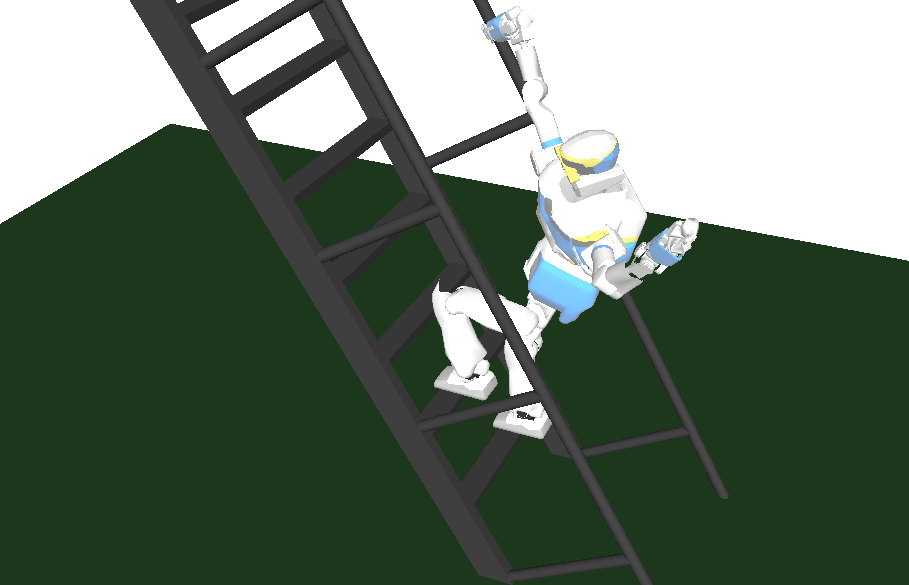
\includegraphics[width=\linewidth]{papers/IROS2014/figure/hrp2_ladder_darpa.png}}
%  %\fbox{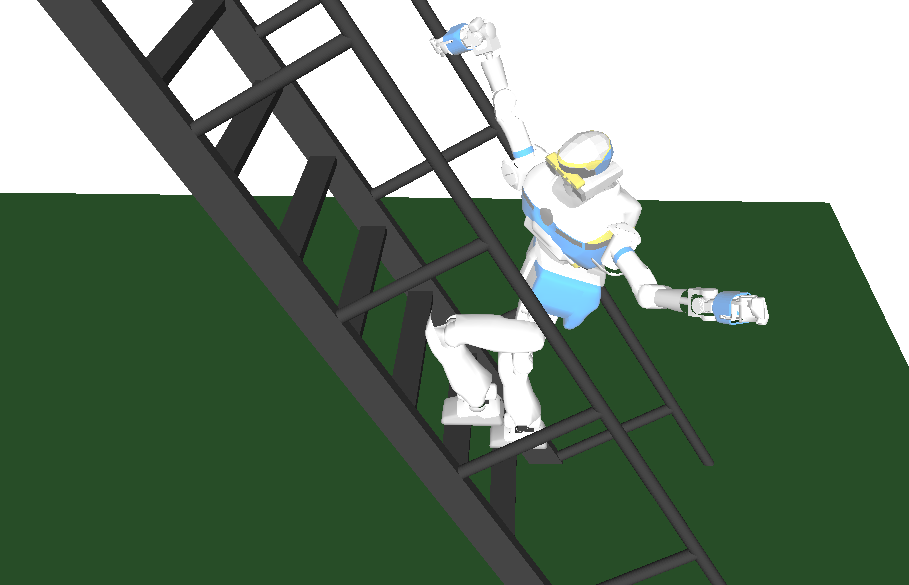
\includegraphics[width=\linewidth]{figure/hrp2_ladder_darpa_40.png}}
%  \fbox{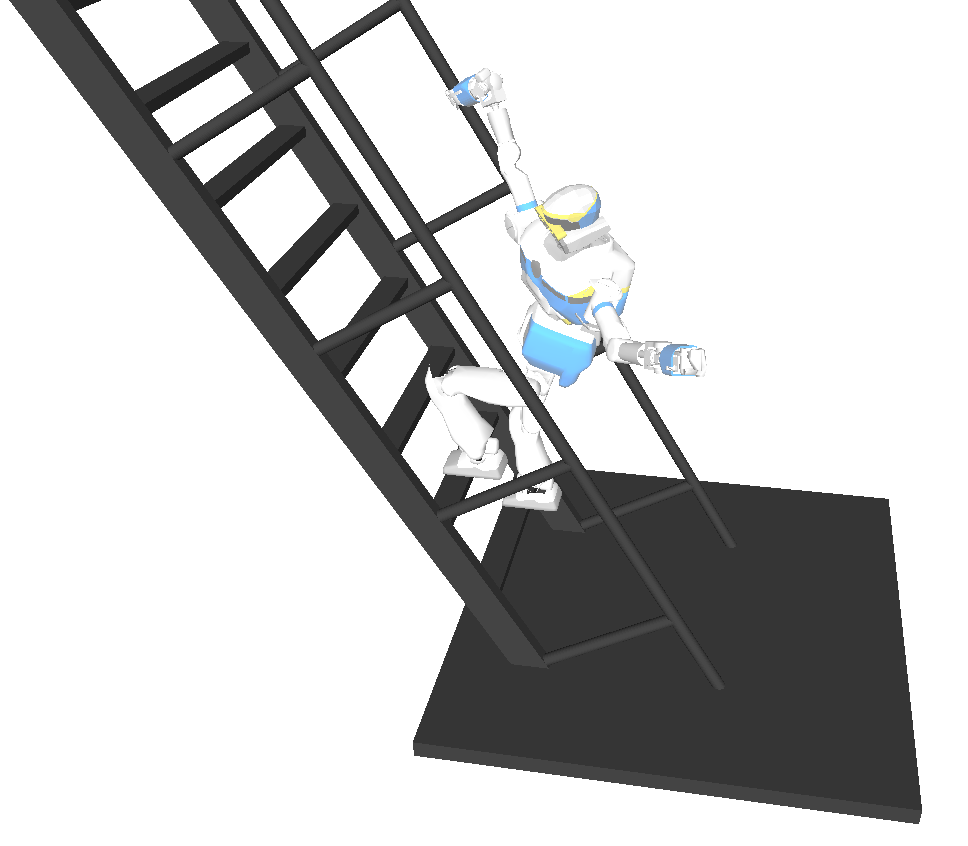
\includegraphics[width=\linewidth]{figure/hrp2_darpa_small.png}}
%  %\caption{HRP2-10 ladder climbing posture}
%  \label{fig:hrp2_darpa}
%\end{subfigure}%
%\begin{subfigure}{.5\textwidth}
%  \centering
%  \setlength\fboxsep{0pt}
%  \setlength\fboxrule{1pt}
%  %\fbox{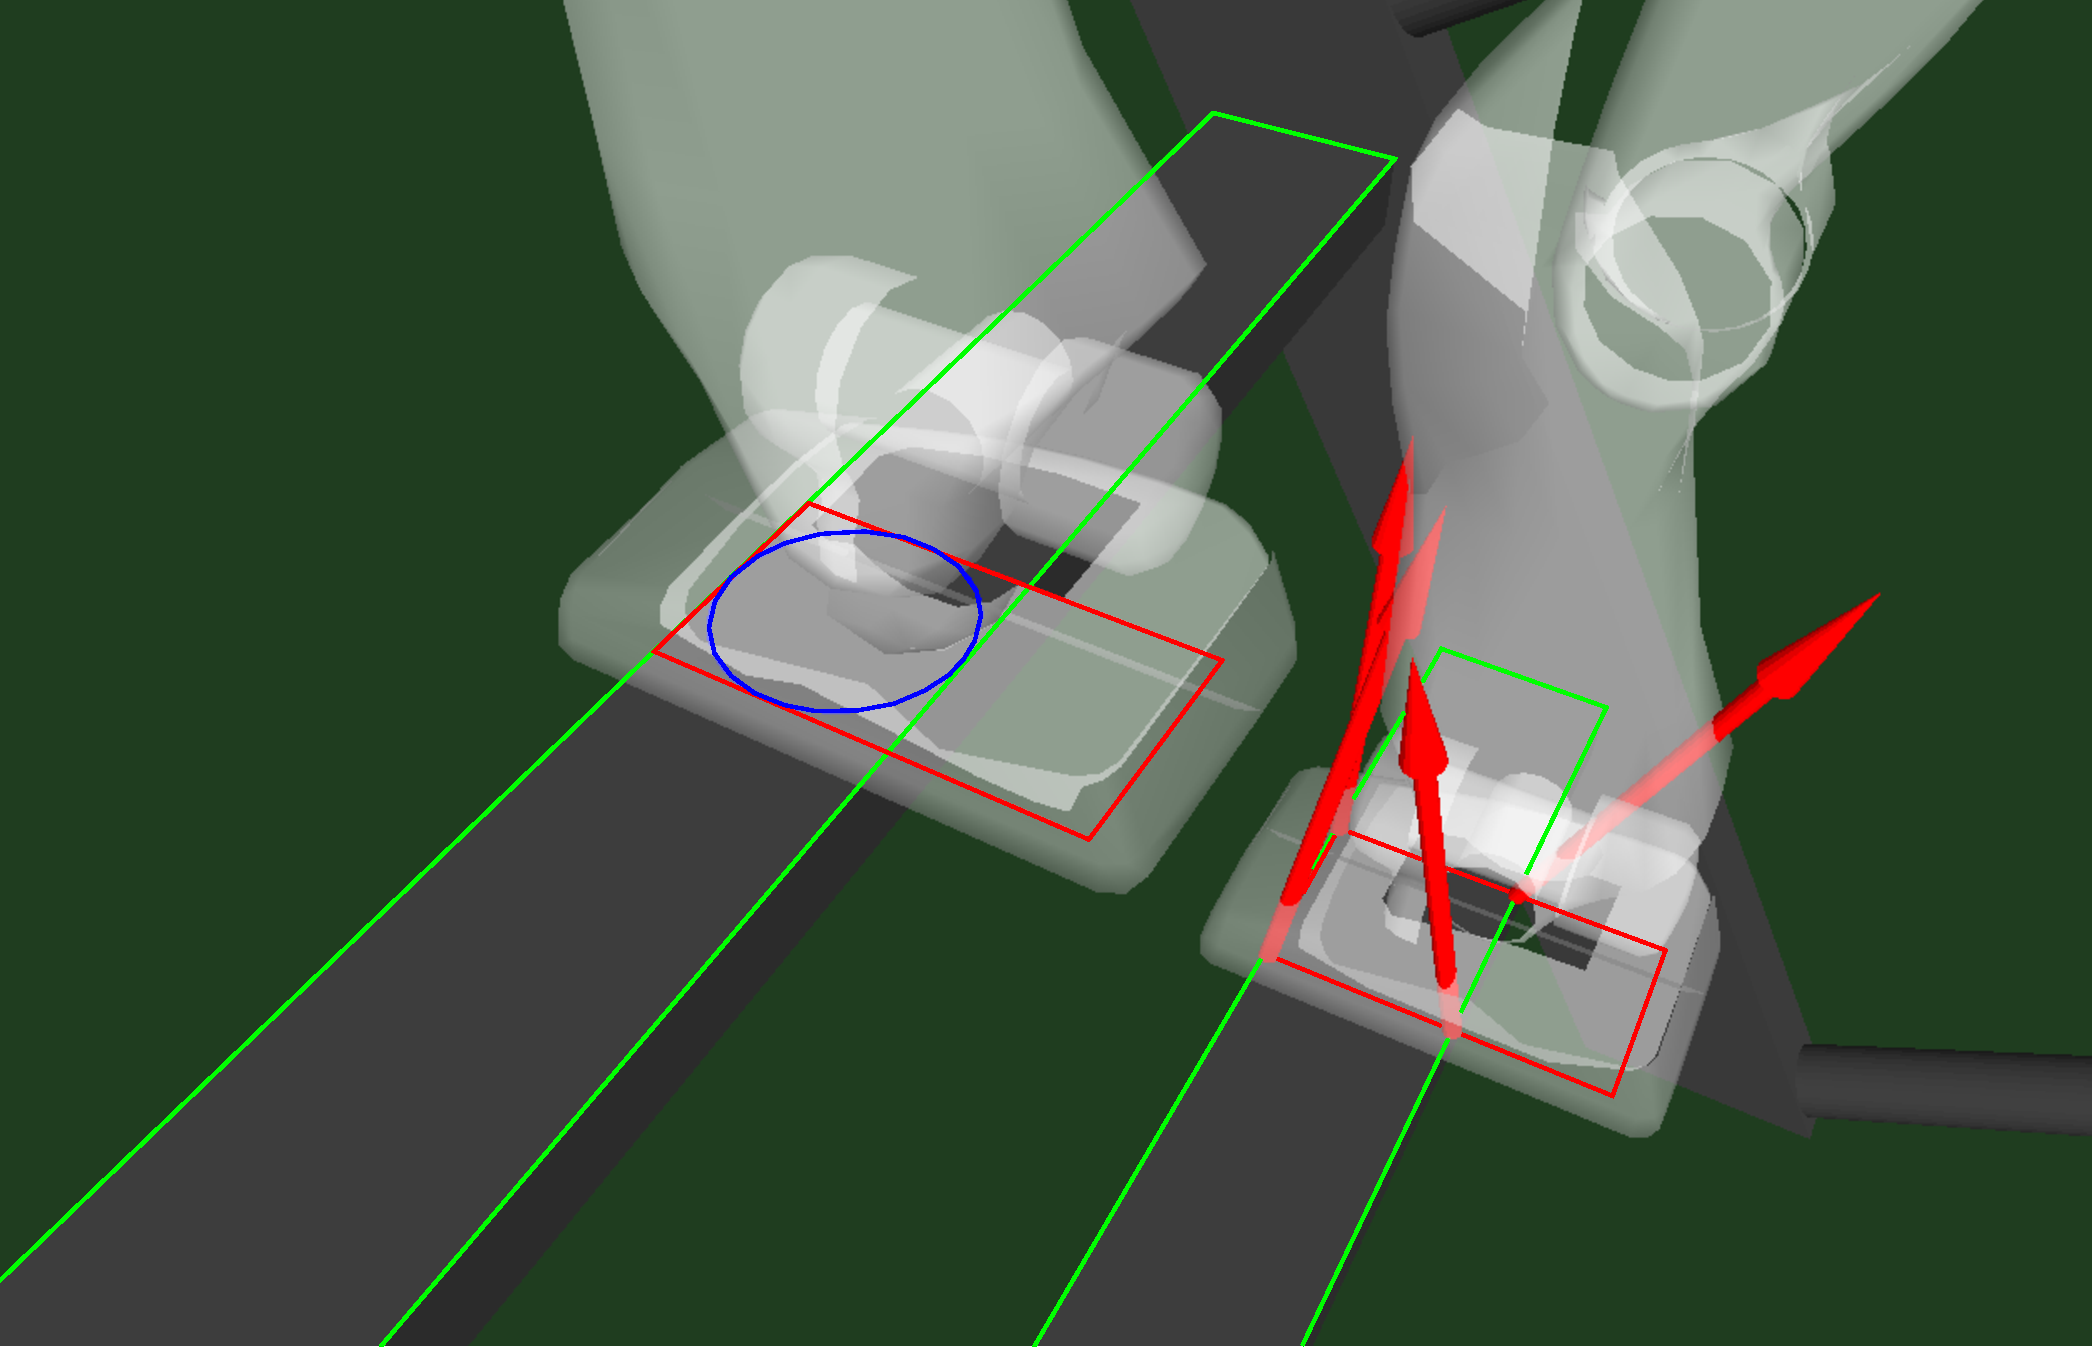
\includegraphics[width=\linewidth]{figure/hrp2_ladder_darpa_zoom.pdf}}
%  %\fbox{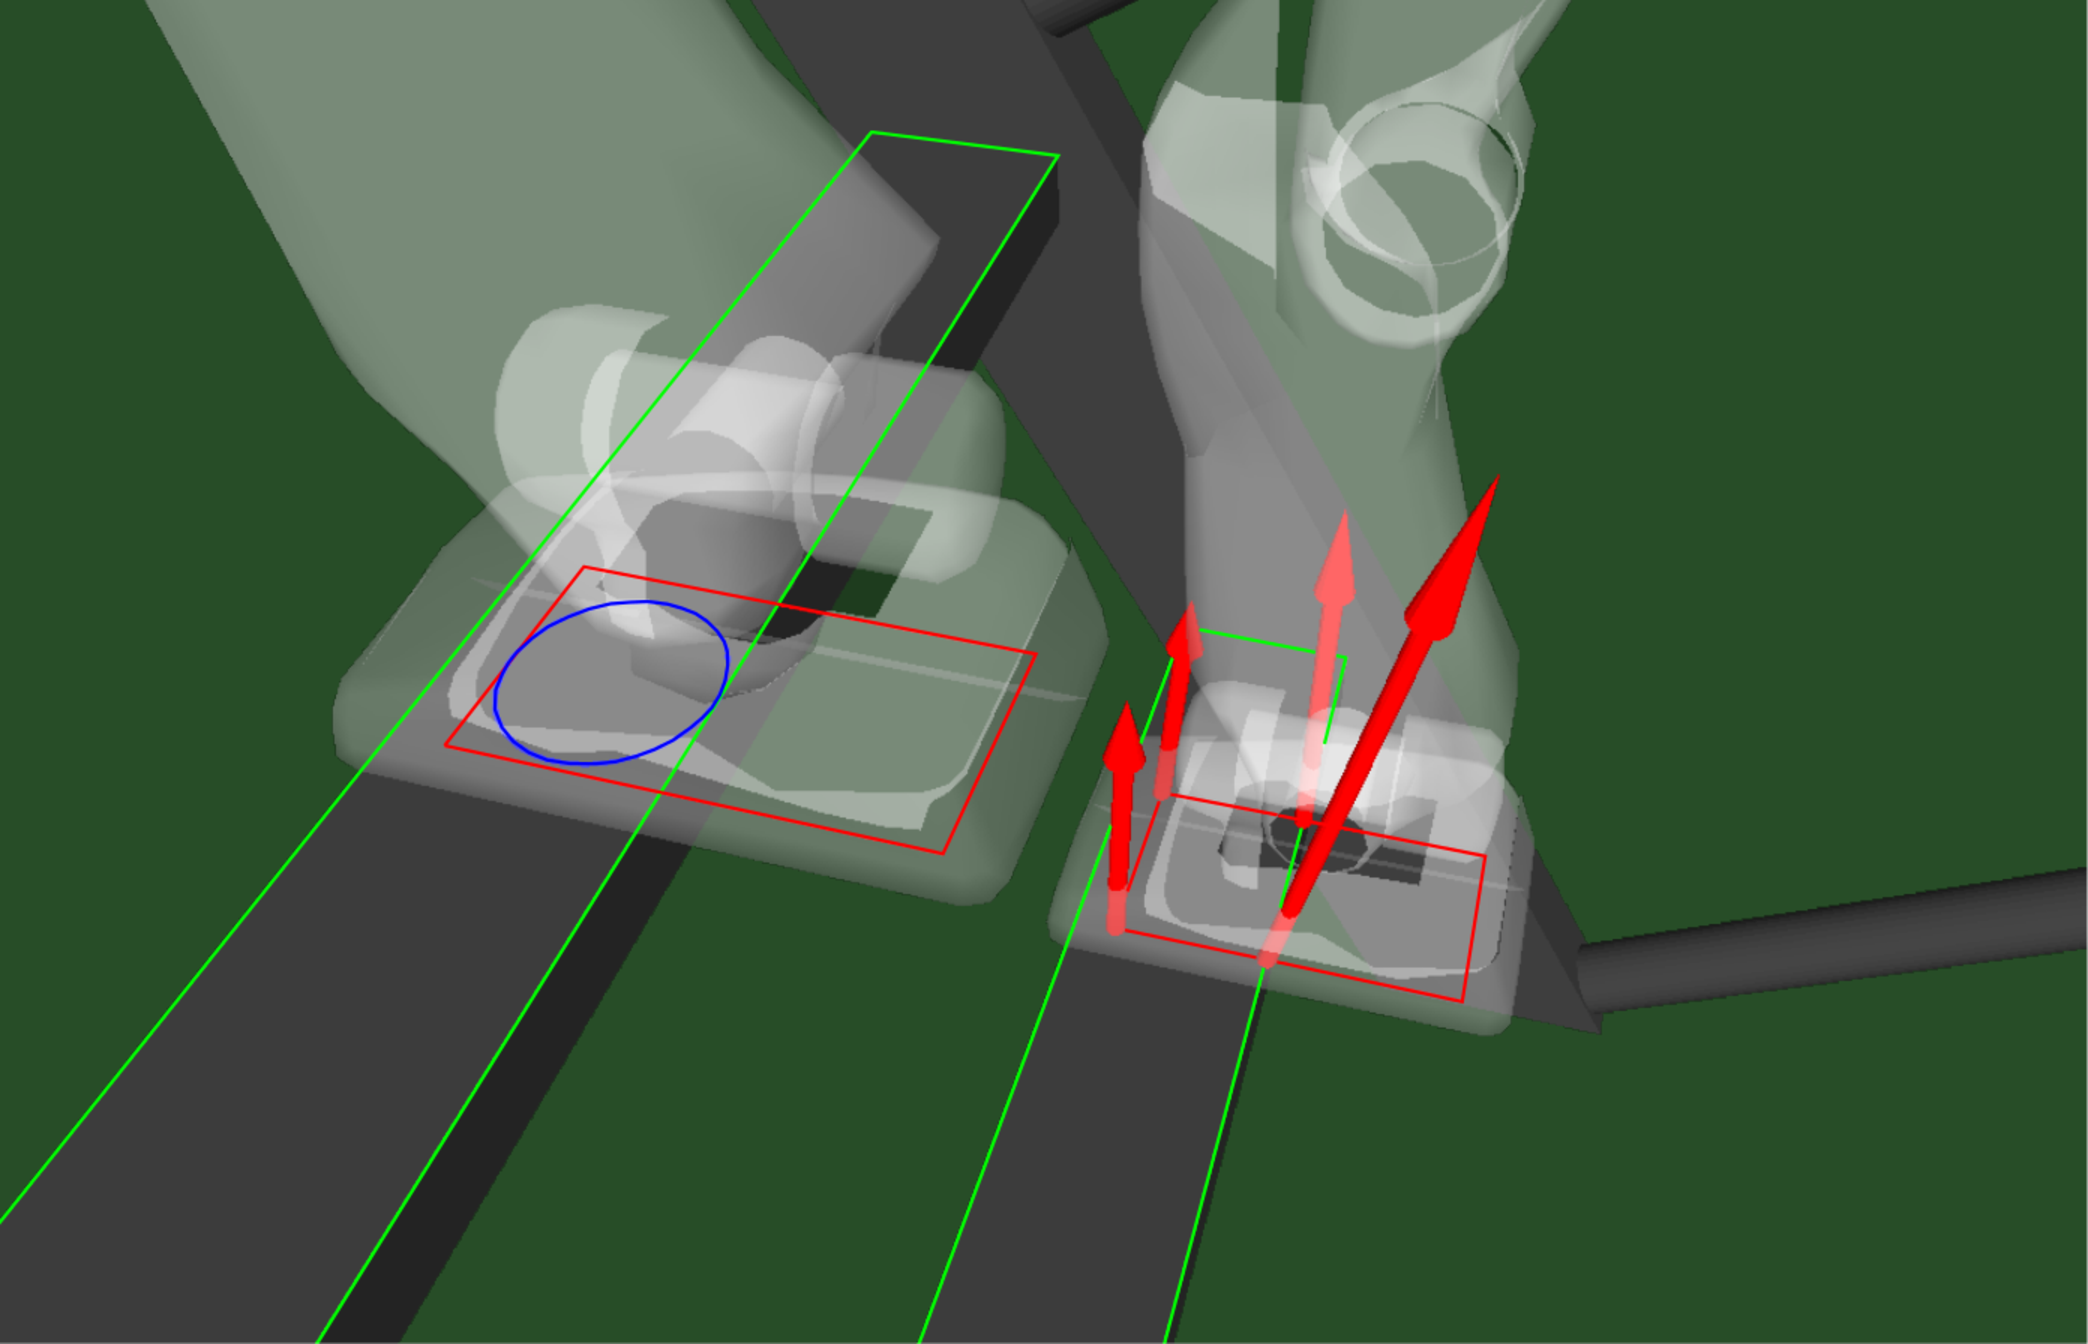
\includegraphics[width=\linewidth]{figure/hrp2_ladder_darpa_40_zoom.pdf}}
%  \fbox{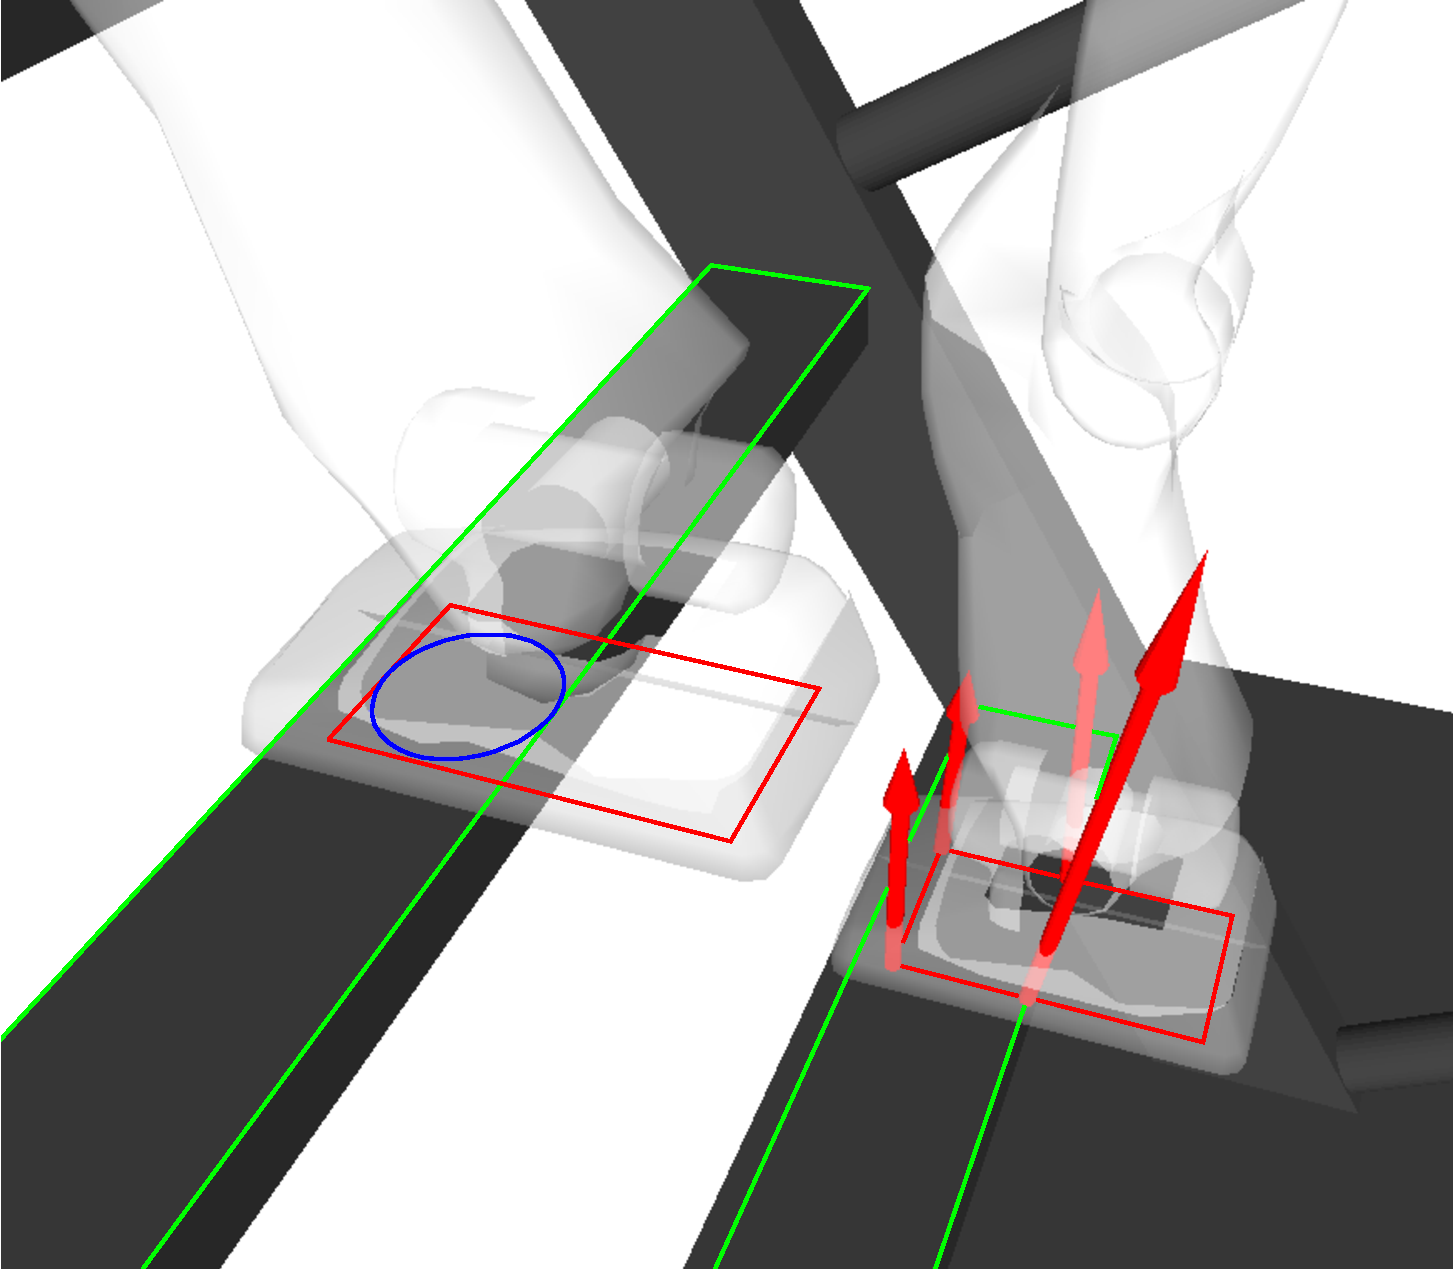
\includegraphics[width=\linewidth]{figure/hrp2_darpa_small_zoom.pdf}}
%  %\caption{Upclose view of the contact areas (green and red: contact polygon, blue: ellipse found in contact area, Red arrows: contact forces resultants)}
%  \label{fig:hrp2_darpa_zoom}
%\end{subfigure}
%\caption{(a)HRP2-10 ladder climbing posture; (b)Upclose view of the contact areas\\(green/red: contact polygons; blue: ellipse found in contact area; red arrows: contact forces resultants)}
%\label{fig:hrp2_darpa_complete}
%\end{figure*}  
\begin{figure}
\centering
\begin{subfigure}{.3325\columnwidth}
  \centering
  \setlength\fboxsep{0pt}
  \setlength\fboxrule{1pt}
  \fbox{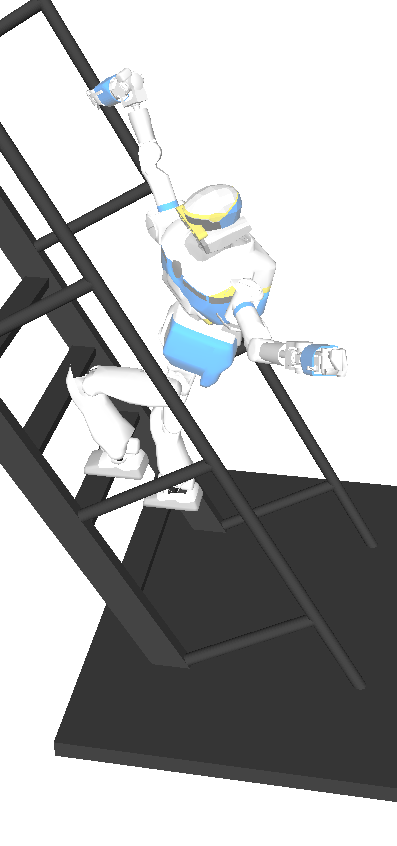
\includegraphics[width=\linewidth]{papers/IROS2014/figure/hrp2_darpa_small_cut.png}}
  \label{fig:hrp2_darpa}
\end{subfigure}%
\begin{subfigure}{.6175\columnwidth}
  \centering
  \setlength\fboxsep{0pt}
  \setlength\fboxrule{1pt}
  \fbox{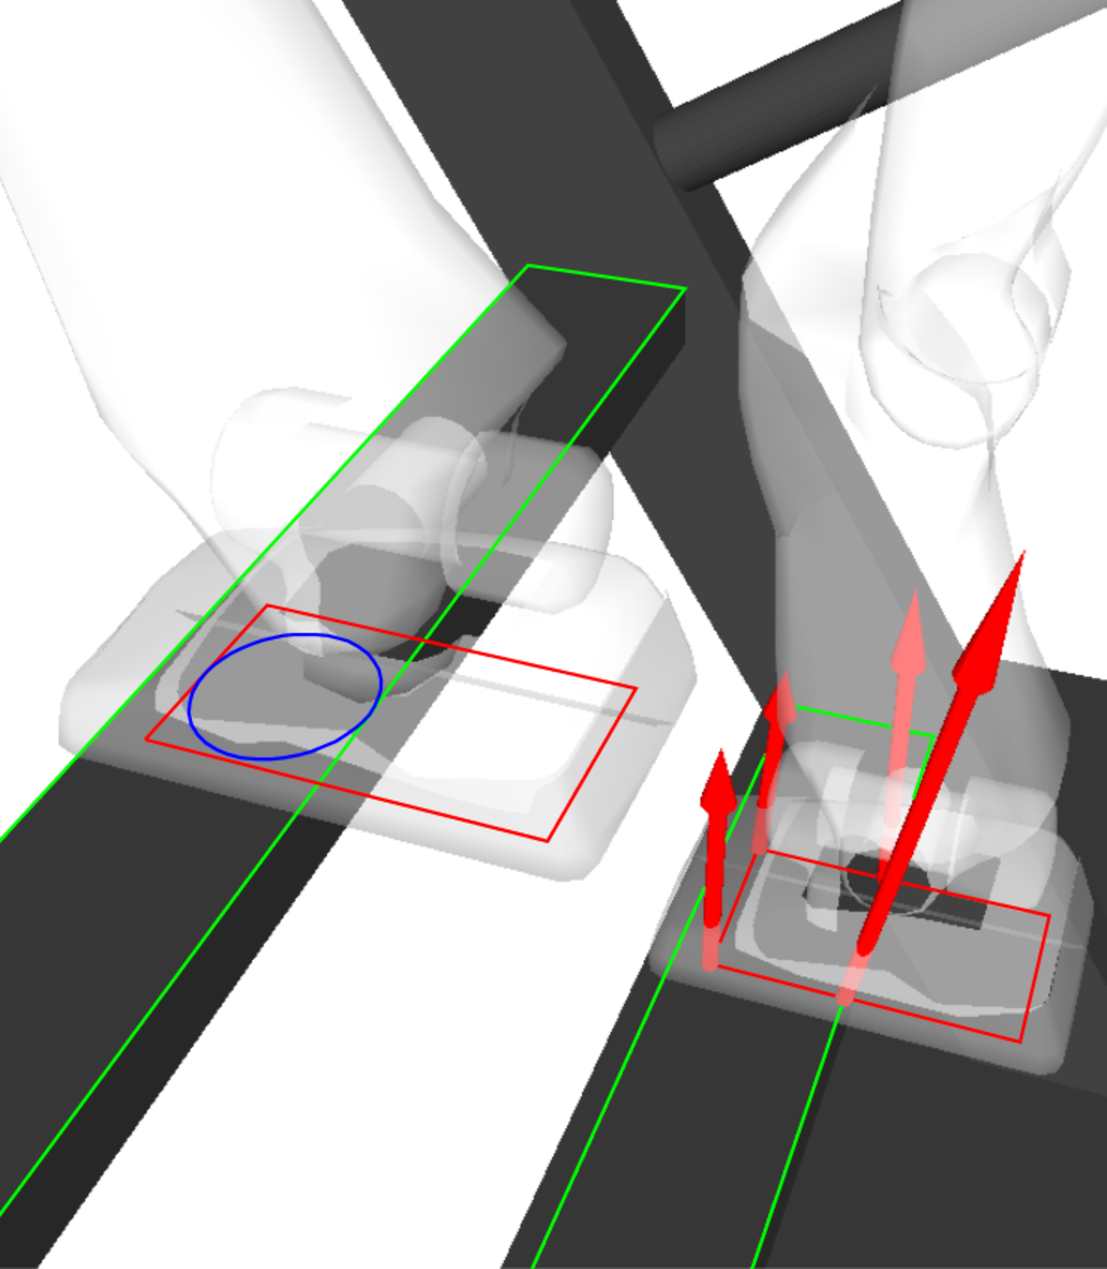
\includegraphics[width=\linewidth]{papers/IROS2014/figure/hrp2_darpa_small_zoom_cut.pdf}}
  \label{fig:hrp2_darpa_zoom}
\end{subfigure}
\caption{HRP2-10 ladder climbing posture and up close view of the contact areas (green/red: contact polygons; blue: contact ellipse; red arrows: contact forces resultants)}
\label{fig:hrp2_darpa_complete}
\end{figure}

\begin{figure*}
\centering
\setlength\fboxsep{0pt}
\setlength\fboxrule{1pt}
\fbox{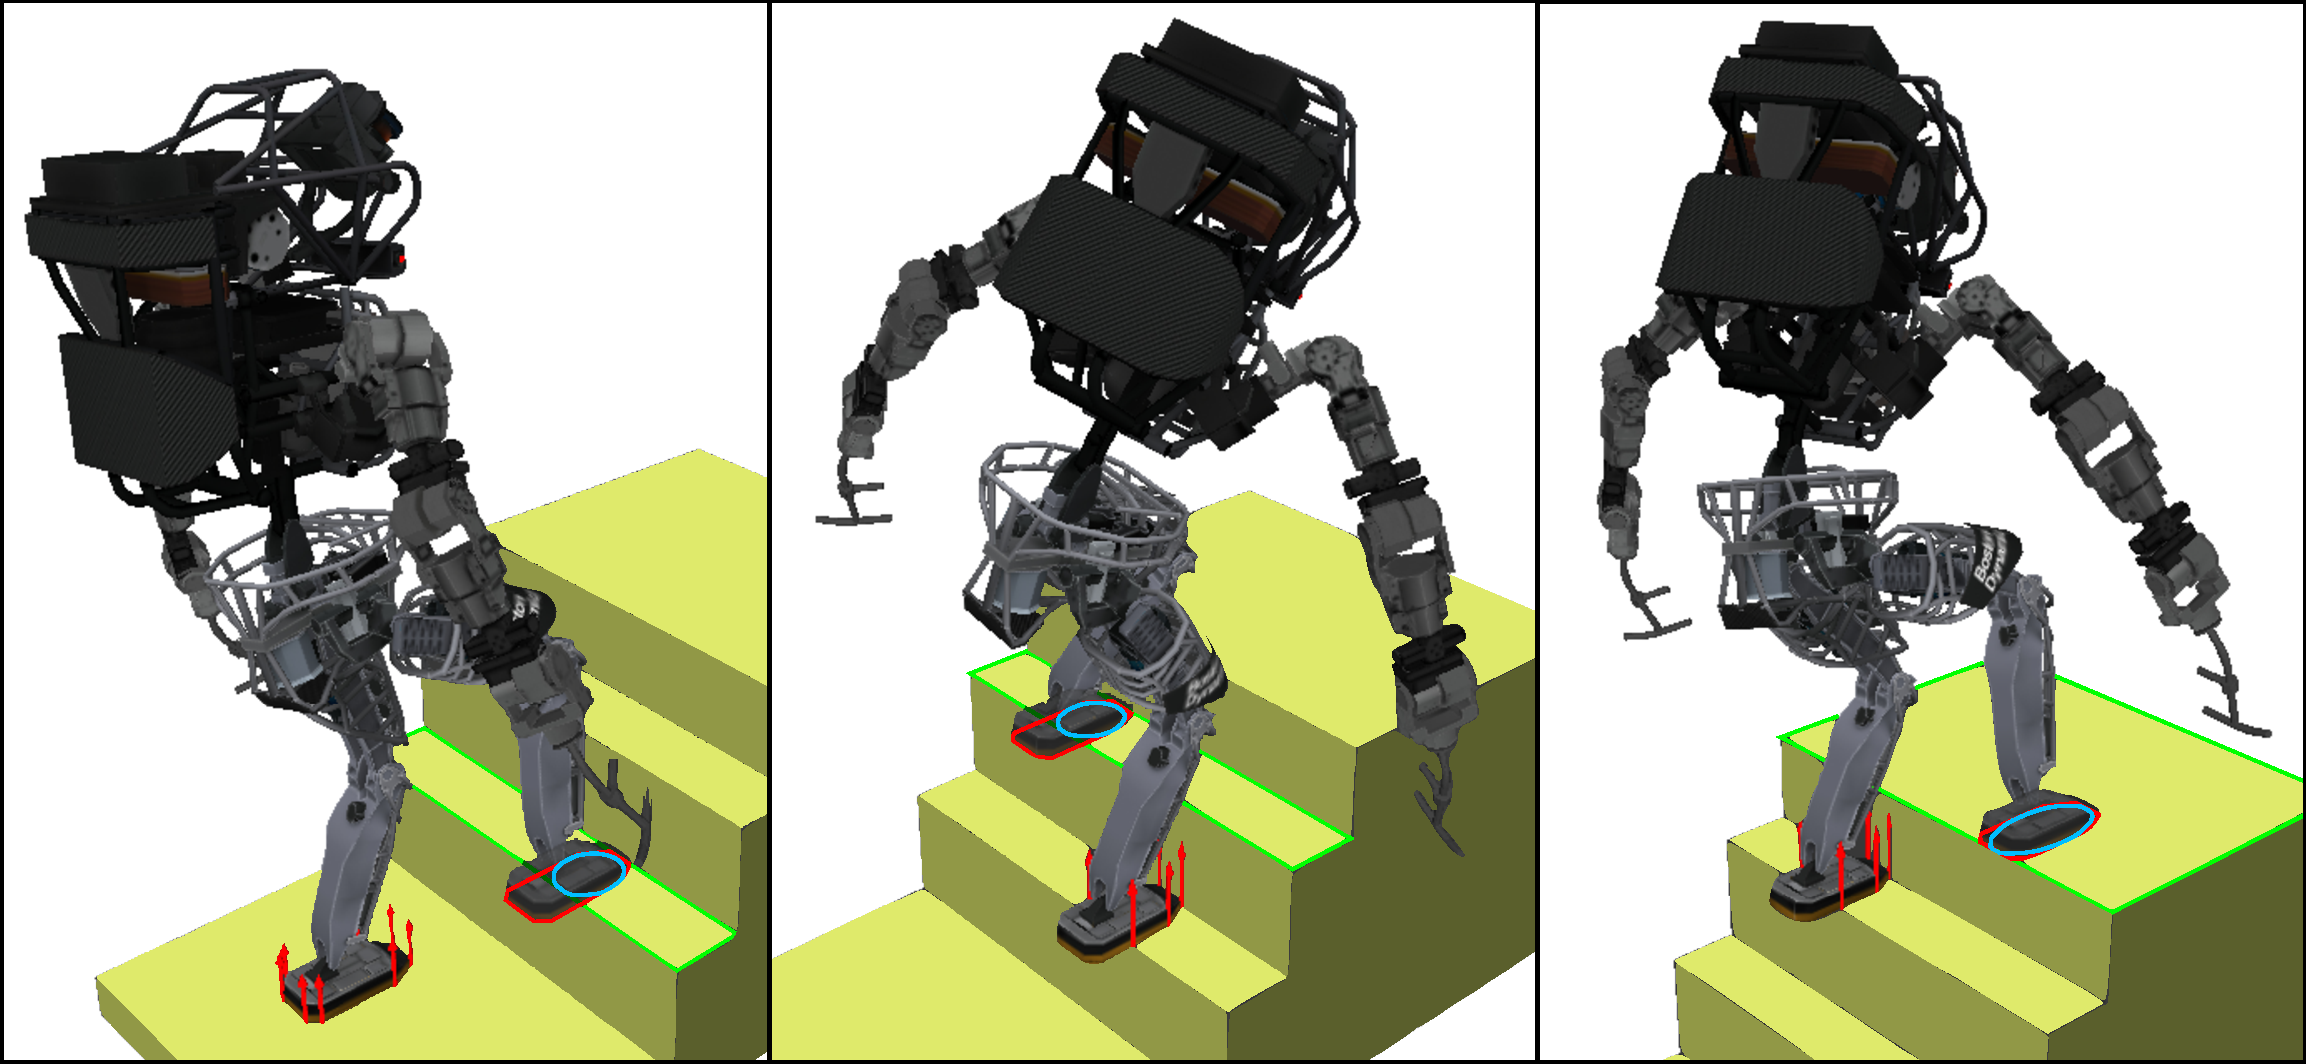
\includegraphics[width=0.95\linewidth]{papers/IROS2014/figure/atlas_1_2_3_yellow.pdf}}
\caption{Atlas climbing stairs with small steps by maximizing the size of the contact areas\\(green/red: contact polygons; blue: contact ellipse; red arrows: contact forces resultants)}
\label{fig:atlas_SmallStairs}
\end{figure*}  

\subsection{Vertical ladder climbing}
\label{subsec:ladder}

In the second example we generate a posture in which the robot climbs a vertical ladder.
In this particular step, the robot is using its right foot and both hands to maintain its stability on top of the first rung of the ladder. We search a posture that keeps those previous contacts and adds a geometrical contact between the left foot and the second rung of the ladder.
The result of that optimization can be observed on ~\Figref{fig:hrp2_jrl_complete}, with the robot posture on the left and a close-up look at the contact areas on the right.
The difficulty of this situation is that a contact has to be made with a very thin surface of the environment (the ladder rung). Usual contact generation method would reduce a lot the span of possible contact position (by patching the robot's foot with a very small surface or by imposing a set of authorized contact positions).
Whereas with our method, the contact configuration is found during the optimization process without requiring any extra human work. The contact chosen by our software includes an ellipse which first axis is the width of the robot's foot and second axis is as thin as the ladder rung.   
One problem to expect is that numerical instability might happen if the surface of the rung is given too thin. But that would also happen with full inclusion constraints.
This example also illustrates one limitation of our method: it only considers planar contacts and if one wants to model a purely linear contact an other contact model must be used, since our modeling of those singular cases is approximative.
%is the first step of the HRP-2 robot climbing a ladder. The two hands are in bilateral contact with the two side bars of the ladder, the left foot is fixed on the ground and is the only part of the robot involved in the stability. The right foot is to make a contact with the first rung of the ladder. The rungs of the ladder are modeled by rectangles with a 6mm width which approximates the contact line as explained in section~\ref{subsec:singular cases}. %Therefore, the ellipse area maximization takes place in the intersection of the polygons representing the rung and the foot. 
%The result of that optimization can be observed on ~\Figref{fig:ladder}{}.
%On the right of the simulation image is shown the disposition of the foot (in green) that is in geometrical non inclusive contact with a rung (in blue) and the optimal ellipse that has been found.


%From a planning point of view, this particular result is obviously not achievable as the right leg of the robot goes through the ladder, this will be discussed in the next section. Yet, the posture is perfectly valid as it respects of the constraints of problem~(\ref{eq:PG}). This example illustrates our method in a multi-contact environment with almost linear contacts. 
%

\subsection{Climbing Stairs}
\label{subsec:smallStairs}

In a third simulation, the ATLAS robot climbs a flight of stairs.
All the steps are too small for the robot to put its entire foot on.
Therefore, it has to make a non inclusive contact and we propose to maximize the size of the contact area with the ellipse included in it, as explained in \ref{subsec:optim-ellipse-area}. 
The size of the contact area is limited by the fact that the foot cannot penetrate the wall behind each step.
On~\Figref{fig:atlas_SmallStairs}, we present 3 postures generated on this environment.
On each of those postures, we see that the ellipse's size is maximized until the foot enters in collision with the vertical wall behind each step. And when possible, like on the last step, the contact area is maximized without collision limitation and the foot is positioned as fully included in the support surface.
We can see here that even when the size of the ellipse is maximized while competing with other non-linear constraints like collision avoidance, our method still works well and leads us to a satisfactory solution.

%Under each simulation result, an image presents the disposition of the foot (in green) that is in geometrical non inclusive contact with a step (in blue) and the optimal ellipse that has been found.
%It has to be noted that the green contact surface under a foot of the robot (green rectangle) is actually smaller than the actual foot due to our use of security margin for stability reason when experimenting with real robot and take into account an un-modeled flexibility at the ankle.
%That is why, with the collision avoidance activated between the foot and the next step, it seems that the foot is still far from the limit of the step (blue rectangle).
%Actually the foot is almost in collision with the vertical part of the next step.
%We decided not to present the initial and final steps of this hypothetical movement because they do not bear any interesting aspect as they both consist of the robot standing on a large flat surface.

%\begin{figure*}
%\centering
%\begin{subfigure}{.319\textwidth}
%  \centering
%  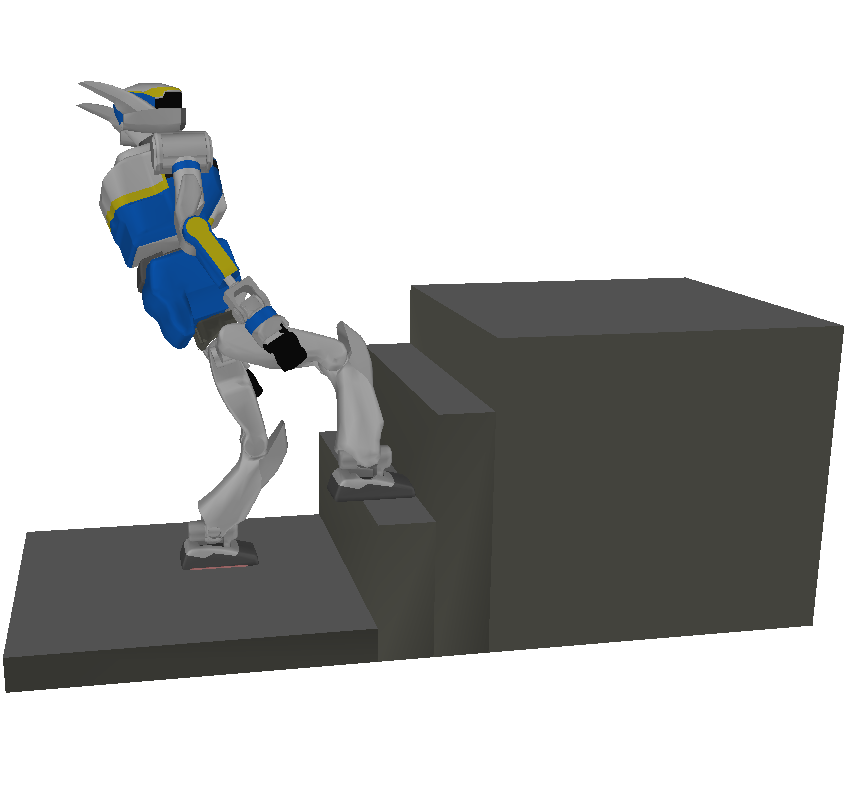
\includegraphics[width=\linewidth]{figure/SmallStairs2.png}
%\end{subfigure}%
%\begin{subfigure}{.3\textwidth}
%  \centering
%  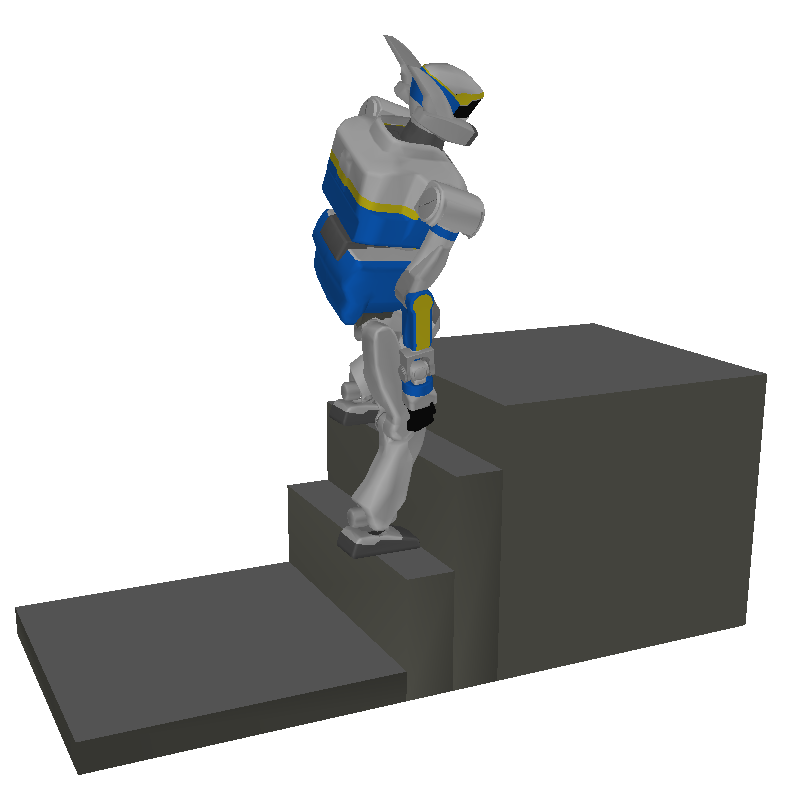
\includegraphics[width=\linewidth]{figure/SmallStairs3.png}
%\end{subfigure}
%\begin{subfigure}{.3\textwidth}
%  \centering
%  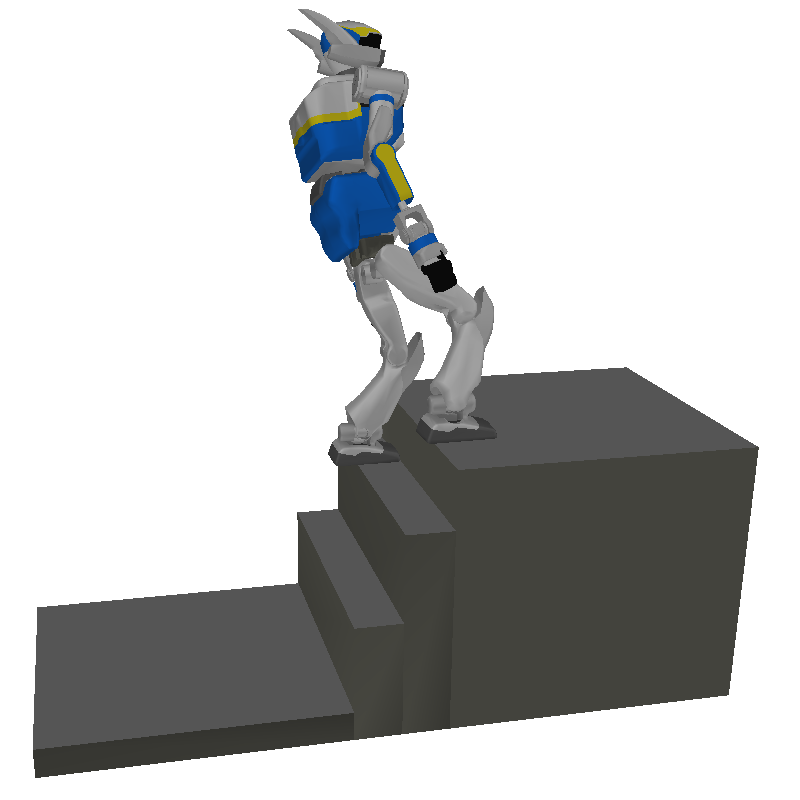
\includegraphics[width=\linewidth]{figure/SmallStairs4.png}
%\end{subfigure}
%\caption{Using non-inclusive contacts for ladder climbing}
%\label{fig:hrp2_SmallStairs}
%\end{figure*}  

%\subsection{Walking along a path made of small objects}
%
%In the second simulation, the HRP-2 robot has to cross a gap by making contacts
%with small surfaces. As well as for the previous simulation, the two objects
%with which the feet of the robot will be in contact are too small for making a
%complete contact, instead, non inclusive geometric contacts are found by
%maximizing the area of an ellipse that fits in the intersection of the polygons
%involved in the contact. Results are presented in ~\Figref{fig:riviere}. As
%we can see, the feet turns slightly, to be more aligned with the support
%surfaces, yet they do not become completely aligned with these supports, which would permit to get the biggest ellipse area. This is due to the fact that a posture cost is competing with the area cost, yielding this compromise.
%%Under each simulation result, an image presents the disposition of the foot (in green) that is in geometrical non inclusive contact with a step (in blue) and the optimal ellipse that has been found. We decided not to present the initial and final steps of this hypothetical movement because they do not bear any interesting aspect as they both consist of the robot standing on a large flat surface.
%
%\label{subsec:riviere}
%\begin{figure*}[!htb]
% \centering
% 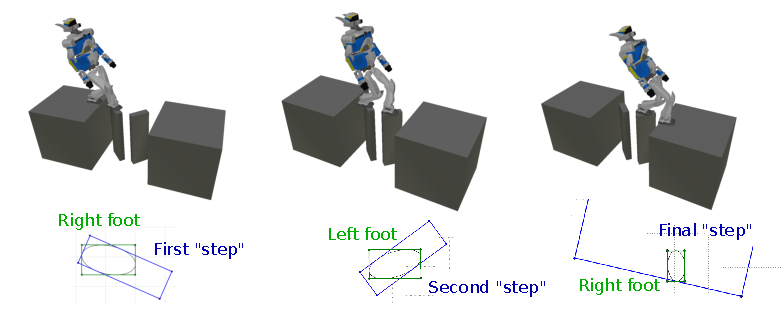
\includegraphics[width=0.75\textwidth]{figure/riviere3steps.pdf}
% \caption{Simulation results for crossing a gap by walking on small items}
% \label{fig:riviere}
%\end{figure*}
%
\section{Discussion and conclusion}
Generating arbitrary shaped contact areas proved to be doable very simply in an optimization-based posture generation module. We focused on writing constraints that have continuous gradients, since the posture generate problem is dominantly smooth. Hence, our geometric contact model can be useful for other optimization-based purposes, for example control or trajectory optimization, and any gradient-based descent scheme which handles inequalities (e.g.~\cite{escande:icra:2010}).
While we were expecting an increase of computation time due to the addition of new variables in the problem,
% (5 more for a total of 80-100 variables)
we noticed that the timings obtained with this method are sensibly the same that our previous version of the posture generator with full contact surface inclusion. Consequently, this method offering a richer contact search (exploration) during planning comes without degrading computation time. In fact, it truly allows us to substantially reduce the time spent by the user in ad-hoc tuning the shapes of the contact patches, or fixing the contact positions that were previously done by hand. Also, it is fairly easy to implement and extends a multi-contact planning algorithms like the one described in~\cite{escande:ras:2013}{} to give it richer planning possibilities.

There are several opportunities for future work. For example, we could improve the generality of our contact constraint formulation even further to manage linear and punctual contacts without the approximations we currently use. Also we could extend our method to allow dealing with non-convex surfaces. And finally we would like to apply our method to other fields that use contact generation, like trajectory or control optimization. Our methods extends straightforwardly to point cloud data as far as polygonal patches can be extracted.
%While we were expecting an increase of computation time due to the addition of new variables in the problem (5 more for a total of 80-100 variables), we were surprised by the obtained timings, around $10s$ while a usual posture generation is less than $1s$. Part of this increase is obviously due to the fact that we used finite differences to compute the gradients of the new constraints and objectives, and one of the immediate on-going works is to derive and implement efficiently analytical gradients. Still, we will also investigate more thoroughly how the new constraints interact with the existing ones to look for potential other causes for this increase.

%Finally, on a planning point of view, ~\Figref{fig:ladder} shows us a new challenge: while the posture found is perfectly correct as the robot is stable, not colliding with its environment and the contacts are where we asked them to be, the posture is obviously difficult to attain, if possible at all. We will need to investigate what type of heuristic to use to avoid this kind of results in the middle of a plan.

%\chapter{Humanoid Posture Generation on non-Euclidean Manifolds}

\section{abstract}
We present a reformulation of the posture generation problem that encompasses non-Euclidean manifolds. 
Such a formulation allows a more elegant mathematical description of the constraints, which we exemplify through some scenarios in the simulation results section.
In our previous work, the posture generation problem is formulated as a non-linear optimization program with constraints expressed only through Euclidean manifolds; we solve the latter problem using on-the-shelf solvers.
Instead, we decided to implement a new SQP solver that is most suited to non-Euclidean manifolds structural objects.
By doing so, we have a better mastering in the way to tune and specialize our SQP solver for robotic problems.


\section{Introduction}
\label{sec:Intro}
Computing robot configurations to meet the requirements of a given set of tasks, within a viable state, is a recurrent problem whose complexity grows with that of the robot. In this paper, we are interested in the following generalized inverse kinematics problem: we search a configuration for which the robot fulfills tasks under constraints of joint limits, auto-collision and non-desired collision avoidance, balance, torque limits, etc. We coined it posture generation. Such a problem is encountered in both planning and control. In both cases, computation time and robustness are critical issues.

We have already proposed various implementations of the humanoid posture generation problem. All of our implementations formulate the problem as a non-linear optimization program to address multi-contact planning. In~\cite{escande:ras:2013}, the multi-contact planner explores the contact space using thousands of HRP-2 humanoid posture generator (PG) queries; we used the FSQP solver~\cite{cfsqp:manual}. In~\cite{bouyarmane:ar:2012}, the PG is extended to handle various humanoid robots and multiple agents, the solver used is IPOPT~\cite{wachter:mp:2006}. In~\cite{vaillant:humanoids:2014} the PG is extended to various contact models and used to generate multiple related postures at once. The latter work and the DRC participation revealed that re-planning on the fly is necessary and having a robust PG is crucial in many situations. Other works also make use of PG, e.g. in~\cite{hauser:humanoids:2005}\cite{Aristidou2009}.

Posture generation has been formulated as a problem over a Euclidean space. Robots variable may however be more naturally expressed over non-Euclidean manifolds. The archetypes for this are the rotation part of the root body for a humanoid robot, and ball joints, whose variables live in $SO(3)$. Some typical tasks are also naturally formulated on different manifolds. For example for making contact with any object that can be mapped on a sphere, the contact point position for this object can be parametrized in $S2$. Human shoulder can be elegantly parametrized on $S2\times\mathbb{R}$, as proposed in~\cite{Baerlocher}.

\begin{figure}[!tb]
\centering
  \centering
  \setlength\fboxsep{0pt}
  \setlength\fboxrule{1pt}
  \fbox{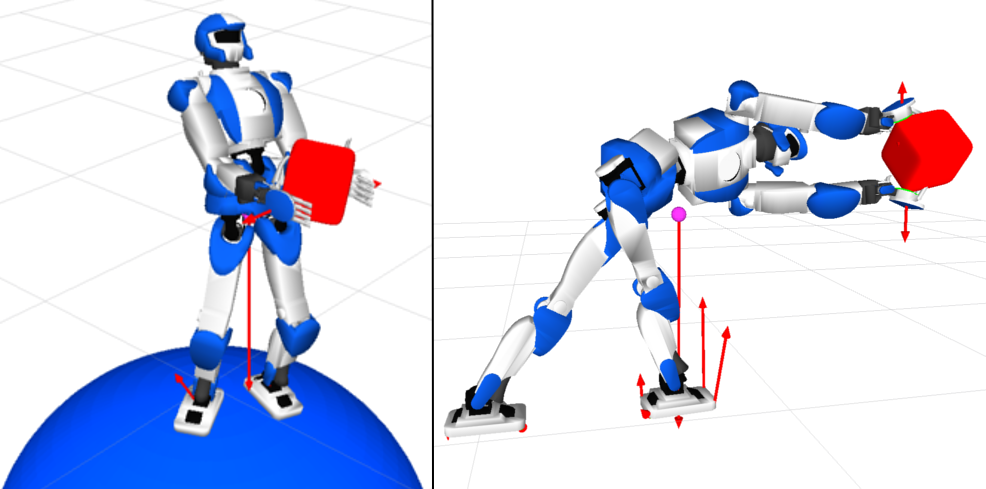
\includegraphics[width=.95\linewidth]{papers/Humanoids2015/figure/hrp4CubeOnSphere.png}}
\caption{HRP-4 carrying a 2-kg cube. Left: feet on a sphere, objective function is to maintain the cube at a given position. Right: right foot free to move on the floor, objective is to put the cube as far as possible in a given direction}
\label{fig:hrp4_cube}
\end{figure}

Formulating the problem over $\mathbb{R}^n$ leads either to discontinuities that can prevent the convergence of the optimization solver, or to cumbersome writing to specify that the variable is actually living on a manifold (see~\cite{bouyarmane:humanoids:2012}).

In this paper, we propose a new optimization solver able to work on generic smooth manifolds. We take inspiration from the approach used for unconstrained optimization on manifold~\cite{absil:book:2008} and adapt it to constrained optimization. To the best of our knowledge, constrained optimization on manifold has drawn few research for now. This is likely due to the fact that in most problems the only constraint is to be on the manifold. We are only aware of the work of Schulman~\emph{et al.}~\cite{Schulman2014}, where the authors explain the adaptation of their solver to work on $SE(3)$. This adaptation is however not valid for general manifolds without more care about hessian computation.

The second contribution of this paper is a Posture Generation framework developed to ease the writing of functions, so that the user can focus on the problem formulation without having to care about the tedious bookkeeping inherent to optimization problems of this size.

A background motivation for this work is to have our own optimization solver, instead of a black box. We will now be able to specialize the solver specifically to robotic problems, by leveraging modeling properties and approximations, for a gain in time and robustness. We also look forward to using this solver for problems with a varying number of constraints along the iterations (such as when complex collision constraints are considered).

The rest of the paper is organized in a classical way: we start with a bit of math to describe the foundations; then we introduce the PG~\emph{per se}, the problem formulation followed with illustration of successful generations. 

\newcommand{\reduce}[2]{\hspace{-#2pt} #1 \hspace{-#2pt}}

\section{Optimization on Manifolds}
\label{sec:1}
In this section, we describe a Sequential Quadratic Programming (SQP) approach~\cite{nocedal:book:2006} to solve the following non-linear constrained optimization program

\begin{align}
\label{eq:optim_problem}
  \minimize_{x \in \mathcal{M}} & \quad f(x)\\
  \text{subject to}&
  \begin{array}{rcl}
    {l} \leq & \reduce{c(x)}{8}& \leq {u} \nonumber
  \end{array}
\end{align}

where $\mathcal{M}$ is a $n$-dimensional smooth manifold and $c$ is a $m$-dimensional real-valued function.

\subsection{Representation problem}
When $\mathcal{M} = \mathbb{R}^n$, the problem~(\ref{eq:optim_problem}) is solved iteratively, starting from an initial guess $x_0$ and performing successive steps $x_{i+1} = x_i + {\bf p_i}$ where ${\bf p_i}$ is the increment found at the $i$-th iteration, until convergence is achieved. The strategy to compute ${\bf p_i}$ depends on the solver.

This classical scheme cannot be readily applied to optimization over non-Euclidean manifolds. First of all, only (a subset of) the real numbers can be stored in computers. To manipulate elements of $\mathcal{M}$ we need to choose a way to represent them in memory. This boils down to choosing a representation space $\mathbb{E} = \mathbb{R}^r$ (with $r \geq n$) and a map
\begin{equation}
  \psi\ :\ 
  \begin{array}{ccc}
    x & \reduce{\mapsto}{6} & \mathbf{x} \\
    \mathcal{M} & \reduce{\rightarrow}{6} & \mathbb{E}
  \end{array} \nonumber
\end{equation}
In the following, we identify $\mathcal{M}$ with the set $\psi(\mathcal{M}) \subseteq \mathbb{E}$.

With this representation, it is tempting to simply transform problem~(\ref{eq:optim_problem}) as an optimization over $\mathbb{R}^r$ with objective $f \circ \psi^{-1}$ and constraint $c \circ \psi^{-1}$, and solve it with a usual solver. But depending on the representation choice, one of the two following problems arises:\\
(i) $r=n$, then it is not possible in the general non-Euclidean case to find $\psi$ without derivative discontinuities. This can lead to critical convergence problems, \\
(ii) $r>n$, then most elements of $\mathbb{E}$ do not represent an element of $\mathcal{M}$ %($\psi(\mathcal{M})$ is a measure-zero subset of $\mathbb{E}$) 
and $\psi$ cannot be surjective. Constraints need to be added to force the solution on $\mathcal{M}$. As a result, the problem has more variables and constraints w.r.t (i). Moreover, the additional constraints are unlikely to be met along the iteration process (even if $x_i$ is an element of $\mathcal{M}$, $x_i+{\bf p_i}$ is likely not, as nothing enforces it). This means that in order to evaluate $f \circ \psi^{-1}$ and $c \circ \psi^{-1}$ at a given $x_i$, one has to project it on $\psi(\mathcal{M})$ first, effectively computing $f \circ \psi^{-1} \circ \pi$ and $c \circ \psi^{-1} \circ \pi$, where $\pi$ is the projection. The composition by $\pi$ is an additional burden in programming (see e.g. in~\cite{bouyarmane:humanoids:2012a}).

As a simple example, the set of 3D-rotations $SO(3)$ is a manifold of dimension $3$. The following (classical) choices can be made
\begin{itemize}
  \item Rotation matrix ${\bf R} \in \mathbb{R}^{3\times 3} \approx \mathbb{R}^9$, additional constraints: $\{{\bf R}^t{\bf R} = I\ ,\ \det({\bf R})=1\}$, projection by orthogonalization,
  \item Quaternion ${\bf q} \in \mathbb{R}^4$, additional constraints: $\{ \left\|{\bf q}\right\|=1\}$, projection $\pi({\bf x}) = {\bf x}/\left\|{\bf x}\right\|$,
  \item Euler angles ($\mathbb{E} = \mathbb{R}^3$), singularities when reaching gimbal lock.
\end{itemize}


\subsection{Local parametrization}
By definition, there is always, at a point $x$ of a smooth $n$-dimensional manifold $\mathcal{M}$, a smooth map $\varphi_x$ between an open set of $T_x\mathcal{M}$, the tangent space to $\mathcal{M}$ at $x$, and a neighborhood of $x$, with $\varphi_x(0) = x$. $T_x\mathcal{M}$ can be identified with $\mathbb{R}^n$. This gives us a local parametrization for $\mathcal{M}$. The driving idea of the optimization on manifolds is to change the parametrization at each iteration. Applying this idea, we can reformulate Problem~(\ref{eq:optim_problem}) around $x_i$ as
\begin{align}
\label{eq:local_problem}
\minimize_{{\bf z} \in T_{x_i}\mathcal{M}} & \quad f \circ \varphi_{x_i}({\bf z}) \\
  \text{subject to}&
  \begin{array}{rcl}
    {l} \leq & \reduce{c \circ \varphi_{x_i}({\bf z})}{8}& \leq {b} \nonumber
  \end{array}
\end{align} 
This is an optimization problem on $\mathbb{R}^n$. If we perform one iteration of a classical solver starting from ${\bf z_0} = 0$, we get an iterate ${\bf z_1}$, which corresponds to the iterate $x_{i+1} = \varphi_{x_i}({\bf z_1})$. We can then reformulate Problem~(\ref{eq:optim_problem}) around $x_{i+1}$, perform a new iteration and repeat the process until convergence.

\begin{figure}[!htb]
	\centering
  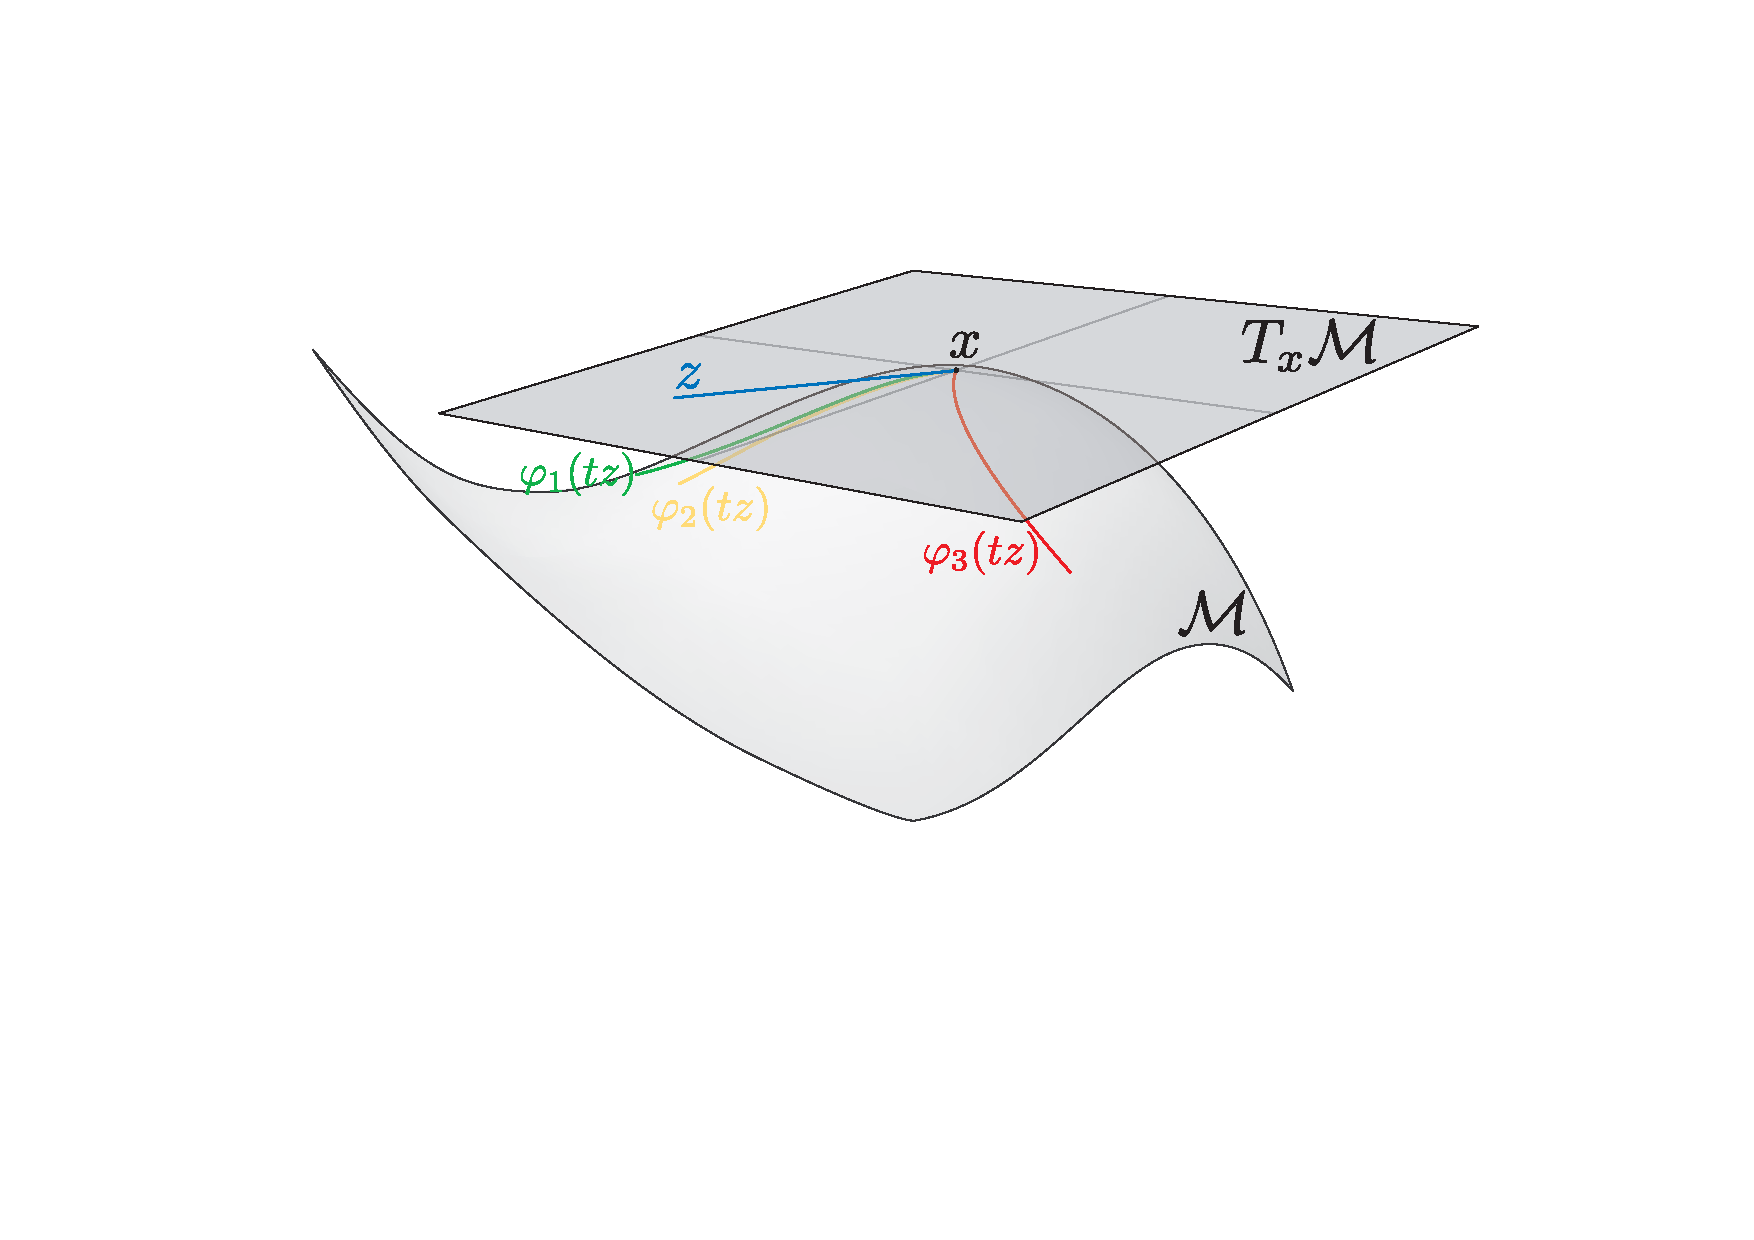
\includegraphics[width=.9\linewidth]{papers/Humanoids2015/figure/manifold.pdf}
    \caption{There are many possible choices for $\varphi_{x}$ but not all yield a curve $\varphi_{x}(t{\bf z})$ which is going in the same direction as ${\bf z}$: $\varphi_{1}$ and $\varphi_{2}$ are correct choices, $\varphi_{3}$ is not.}
	\label{fig:phimap}
\end{figure}


However, convergence cannot be achieved without care on the choice of $\varphi_{x_i}$: it must be such that for any ${\bf z}$, the curve $t \mapsto \varphi_{x_i}(tz)$ is tangent to ${\bf z}$, see Fig.~\ref{fig:phimap}, so that the update $x_{i+1} = \varphi_{x_i}({\bf z_1})$ is made in the direction given by ${\bf z_1}$.

The exponential map is a good theoretical candidate, but it is often impractical or expensive to compute. Depending on the manifold, cheaper maps can be chosen.

With the iterative formulation approach described above, we do not have any parametrization issue, do not need additional constraints, and have the minimum number of optimization parameters. But we still need a map $\psi$ and real space $\mathbb{E}$ to represent the $x_i$ and keep track of them in a global way. The ${\bf x_i}$ are guaranteed to be on $\mathcal{M}$ so we can choose a representation with $r>n$ where $\psi$ is singularity-free without any drawback.
Also, the programmer can write the function $f' = f \circ \psi^{-1}$ as if it was a function from $\mathbb{E}$ to $\mathbb{R}$ without the need to project on $\psi(\mathcal{M})$ first (same goes for $c' = c \circ \psi^{-1}$).
For example if $\mathcal{M} = SO(3)$ and $\mathbb{E} = \mathbb{R}^{3\times 3}$, ${\bf x_i}$ is automatically a rotation matrix and can be used directly as such when writing the function.

\subsection{Local SQP on manifolds}
We choose to adopt an SQP approach to solve our problem. We first define the Lagrangian function
\begin{equation}
  \mathcal{L}_x ({\bf z}, \lambda) = f\circ \varphi_x({\bf z}) - \lambda^T c \circ \varphi_x({\bf z})
\end{equation}
with $\lambda \in \mathbb{R}^m$ the vector of Lagrange multipliers, and note $H_k$ the Hessian matrix $\nabla_{zz}^2 \mathcal{L}_{x_k}$. Taking ${\bf z_0} = 0$, the first SQP step for Problem~(\ref{eq:local_problem}) is computed by solving the following quadratic program

\begin{align}
	\label{eq:SQPStep}
  \minimize_{\bf z \in \mathbb{R}^n } & \quad \frac{\partial f\circ \varphi_{x_k}}{\partial {\bf z}}(0)^T {\bf z } + \frac{1}{2} {\bf z }^T H_k{\bf z }\\
  \text{subject to}&
  \begin{array}{lr}
    \text{l} \leq c\circ \varphi_{x_k}(0) + \frac{\partial c\circ \varphi_{x_k}}{\partial {\bf z}}(0) {\bf z }\leq \text{u}\\
  \end{array} \nonumber
\end{align}

The basic SQP approach adapted to manifolds can be summarized as follows
\begin{enumerate}
	\item set $k=0$ and $x_k$ to the initial value
  \item compute ${\bf z}$ from Problem~(\ref{eq:SQPStep}) for current $x_k$
  \item set $x_k = \varphi_{x_k}({\bf z})$
	\item if convergence is not yet achieved go-to step 2
\end{enumerate}

Computations of function values and derivatives are based on the fact that $f \circ \varphi = f' \circ \psi \circ \varphi$ (and same for $c$), and
\begin{align}
  f'\ :\ 
  \begin{array}{ccc}
    \mathbb{E} & \reduce{\rightarrow}{6} & \mathbb{R}
  \end{array} \nonumber \\
	\psi \circ \varphi\ :\ 
  \begin{array}{ccc}
    \mathbb{R}^n & \reduce{\rightarrow}{6} & \mathbb{E}
  \end{array} \nonumber
\end{align}
are representable functions. The gradient of $f \circ \varphi$ is 
\begin{align}
  \frac{\partial f\circ\varphi_x}{\partial {\bf z}}=
  \frac{\partial f'}{\partial y}(\psi\circ\varphi_x)\times
  \frac{\partial (\psi\circ\varphi_x)}{\partial {\bf z}}
\end{align}

\subsection{Practical implementation}
The above SQP algorithm works locally, \emph{i.e.} when starting close enough to the solution. In practice, various possible refinements are made to ensure convergence from any starting point. We detail hereafter our choices.

Maps $\varphi_{x_i}$ are only valid locally, and we need to account for this: a step ${\bf z}$ found by Problem~(\ref{eq:SQPStep}) should not be outside the validity region of the map. We could enforce this by adding a constraint ${\bf z}_{\text{map}}^- \leq {\bf z} \leq {\bf z}_{\text{map}}^+$ in~(\ref{eq:SQPStep}). This leads naturally to trust region methods that we therefore favor over line-search approaches.

To know if a step ${\bf z}$ is acceptable or not, one usually uses a penalty-based merit function. In our early tests, the update of the penalty parameters proved to be difficult with our types of problems. We now use a filter instead.

Our algorithm is an adaptation of Fletcher's filter SQP~\cite{Fletcher:mathprog:2000} to the case of manifolds: we use an adaptive trust-region that is intersected with the validity region of $\varphi_{x_i}$, and a new iterate $x_{i+1} = \varphi_{x_i}({\bf z})$ is accepted if either the cost function or the sum of constraint violations is made better than for any previous iterates.

Aside from the manifold adaptation, our main departure from Fletcher is in the Hessian computation where we used an approximation, since the exact one is too expensive to compute in our problems. After testing several possibilities, we settled for a self-scaling damped BFGS update~\cite{nocedal:mp:1993,nocedal:book:2006}, adapted to the manifold framework. More precisely, given the Hessian approximation $H_k$ at iteration $k$, we compute the approximation $H_{k+1}$ as follows
\begin{align}
	&s_k = \mathcal{T}_z(z), \quad y_k = \nabla_z \mathcal{L}_{x_{k+1}}(0,\lambda_{k+1}) - \mathcal{T}_z(\mathcal{L}_{x_{k}}(0,\lambda_{k})) \nonumber\\
	&\theta_k = \left\{\begin{array}{ll} 
		1 & \mbox{if} \; s_k^T y_k \geq 0.2 s_k^T \tilde{H}_k s_k \\
		\frac{0.8 s_k^T \tilde{H}_k s_k}{s_k^T \tilde{H}_k s_k - s_k^T y_k} & \mbox{otherwise}
	\end{array}\right. \nonumber \\
	&r_k = \theta_k y_k + \left(1-\theta_k\right) \tilde{H}_k s_k \quad \mbox{(damped update)} \nonumber \\
	&\tau_k = \min\left(1, \frac{s_k^T r_k}{s_k^T \tilde{H}_k s_k} \right) \quad \mbox{(self-scaling)} \nonumber \\
	&H_{k+1} = \tau_k \left(\tilde{H}_k - \frac{\tilde{H}_k s_k s_k^T \tilde{H}_k}{s_k^T \tilde{H}_k s_k} \right) + \frac{r_k r_k^T}{s_k^T r_k} \nonumber
\end{align}
where $\mathcal{T}_{\bf z}$ is a vector transport along ${\bf z}$ (see~\cite{absil:book:2008}) and $\tilde{H}_k$ is such that for ${\bf u} \in T_{x_{k+1}} \mathcal{M}$, $\tilde{H}_k {\bf u} = \mathcal{T}_{\bf z}\left(H_k \mathcal{T}_{\bf z}^{-1}({\bf u}) \right)$.

Despite Powell's update, $H_{k}$ might not be positive definite (but still symmetric). We regularize it as follows: we first perform a Bunch-Kaufman factorization $P_k H_k P_k^T= L_k B_k L_k^T$ where $P_k$ is a permutation matrix, $L_k$ is unit lower triangular and $B_k$ is block diagonal with blocks of size $1 \times 1$ or $2\times 2$ (obtaining $B_k$ as a diagonal matrix is not numerically stable for Cholesky-like decomposition of indefinite matrices), see~\cite{golub:book:1996}. 
The eigenvalue decomposition $B_k = Q_k D_k Q_k^T$ is immediate and cheap to compute. From the diagonal matrix $D_k$ we form $D'_k$ such that $d'_{ii} = \max\left(d_{ii},\mu_{\min}\right)$ where $\mu_{\min}>0$ is user-defined (we typically set it to $0.1$). 
Defining $L'_k = L_k Q_k (D'_k)^{1/2}$, we get a regularized matrix $H'_k = P_k^T L_k L_k^T P_k$. In our case, we use {\tt LSSOL}~\cite{gill:techrep:1986} for solving the QP~(\ref{eq:SQPStep}), which directly accepts the factorized form $(P_k, L'_k)$. This avoids an internal Cholesky factorization so that our regularization does not add too much time to the overall process of building and solving the QP.

The code for $\psi\circ\varphi$, its gradient and the vector transport needs only to be implemented once for each elementary manifold (it is then trivial to get those functions for Cartesian products of manifolds). The composition with $f'$ and $c'$ is done automatically. The expression of those functions is adapted from~\cite{boumal:jmlr:2014}.

\section{Posture Generation, variables and architecture}
\label{sec:2}

Writing a posture generation problem can easily become cumbersome without the appropriate tools. 
Common pitfalls are for example writing the derivative of a function, managing how the Jacobian matrices of the already implemented functions are modified when a variable is added to the problem, adding a new type of constraint, or correctly writing a function on a sub-manifold of the problem manifold. 
A fair amount of bookkeeping is always necessary, which should not be the charge of the user writing the constraints.
In our PG, we propose an architecture automating most of the problematic tasks, so that the user can focus on the mathematical formulation of the problem.
%\begin{itemize}
  %\item A system of geometrical and mathematical expression trees that automatically computes the mathematical expressions behind geometric relations
  %\item An automatic mapping between the submanifold of each function and the global manifold of the problem
  %\item A problem generator that aggregates all the informations from the abovementionned items to generate a problem that can be passed to the solver
%\end{itemize}

\subsection{Geometric expressions}

Most constraints are geometric.
In order to simplify the writing of functions, we use a dedicated system of expression graph encapsulated in a set of geometric objects.
The main idea is to separate the purely mathematical logic from the geometric one. As an example if $P_r$ and $V_r$ are a point and a vector attached to the camera of the robot, and $P_e$ is a fixed point in the environment, the constraint $(P_e - P_r).V_r = 0$ can be used to have the robot look at $P_e$. With our system, the user creates only those objects and write the code {\tt (Pe-Pr).dot(Vr)} to get the value needed. The geometric layer takes care that all the quantities are expressed in the correct frame, the mathematical layer performs the corresponding operations. If $q$ is a variable object, {\tt (Pe-Pr).dot(Vr).diff(q)} returns automatically the differential of the expression w.r.t. $q$. This makes the writing of the constraints very easy.

At the mathematical level, we consider 5 types of expressions which can be either variables or constants:
\begin{itemize}
  \item Scalar, a 1-dimensional element of $\mathbb{R}$
  \item Coordinates, a 3-dimensional element of $\mathbb{R}^3$
  \item Rotation, a $3\times3$ matrix representing a 3D rotation
  \item Transformation, a $4\times4$ matrix representation of a 3D isometry
  \item Array, a dynamic size array
\end{itemize}
The meaningful unary (inverse, opposite, norm...) and binary (multiplication, addition, subtraction, dot product...) operations (with their derivatives by chain rule) are implemented.
We also have a Function class for more complicated expressions, for example expressing $q \mapsto T_i(q)$ where $T_i$ is the transformation between the reference frame of the robot and the frame of its $i$-th body \footnote{The kinematics of rigid body systems is handled by the RBDyn library (\url{https://github.com/jorisv/RBDyn})}. 
The combinations of those elementary operations defines a computation graph.%, just like in many symbolic calculation frameworks.

The geometric layer consists of physical or geometric objects, named features, which exist independently of their mathematical expression in a given reference frame. We have so far 4 objects:
\begin{itemize}
  \item A Frame, defined by a Transformation expression and a reference frame. 
  \item A Point and a Vector, defined by a Coordinates expression and a reference frame. 
  \item A Wrench, defined by a pair of Coordinates expressions and a reference frame.
\end{itemize}
We have a special World Frame object to serve as starting reference frame. 

For each feature, one can get its expression in a given frame.
Basic operations are defined between those features (when applicable). For example, the subtraction between two Points gives a Vector. The geometric logic resides in the change of frame and those operations.

%Based on that expression system, the robot can simply be represented as a function that keeps track and updates the transformations of the frames of all its bodies, with respect to an Array expression on entry, the articular parameters.
%For a given articular parameter array, the user can query the frame of any body on the robot, and by composition, the user can query any feature defined on a frame of the robot, as well as its derivatives.
%This tools allows for a very simplified writting of robotics constraints as a combination of operations on geometric features, without worrying about the vectors and matrix beneath and without having to write the derivatives.

\subsection{Automatic mapping}

The manifold $\mathcal{M}$, on which the optimization takes place, is a Cartesian product of several sub-manifolds. Same goes for their representation spaces:
\begin{equation}
  \begin{split}
    \mathcal{M} = \mathcal{M}_1\times\mathcal{M}_2\times\mathcal{M}_3\times\hdots\\
    \mathbb{E} = \mathbb{E}_1\times\mathbb{E}_2\times\mathbb{E}_3\times\hdots
  \end{split}
\end{equation}
From the solver's viewpoint, the entry space of each function is the complete manifold.
But for the developer, writing a function on the complete $\mathbb{E}$ is cumbersome because (i) of the need to manage indexes, and (ii) when the function is implemented, the complete $\mathbb{E}$ may not be known.
A user-written function $f$ is usually defined on a subset of $\mathbb{E}$, say $\mathbb{E}_I=\mathbb{E}_i\times\mathbb{E}_j\times\mathbb{E}_k\hdots$, that is minimalist for that function, and should not account for unrelated manifolds. One does not want to think about the values of the forces when writing a geometric constraint for example.
Our automatic mapping tool %keeps track of all the necessary mappings for each function added and upon the instantiation of the problem, 
generates the correct projection functions $\pi_I$ such that the developer can write a function $f$ on $\mathbb{E}_I$ while the solver receives it as a function $f \circ \pi_I$ on $\mathbb{E}$. This idea is illustrated by the example in Fig.~\ref{fig:auto_map}
%\begin{equation}
  %\begin{split}
  %\pi_I:\mathbb{E}\to\mathbb{E}_I\\
  %f:\mathbb{E}_I\to\mathbb{R}\\
  %f\circ\pi_I:\mathbb{E}\to\mathbb{R}
  %\end{split}
%\end{equation}

\begin{figure}[!htb]
\centering
  \centering
  \setlength\fboxsep{0pt}
  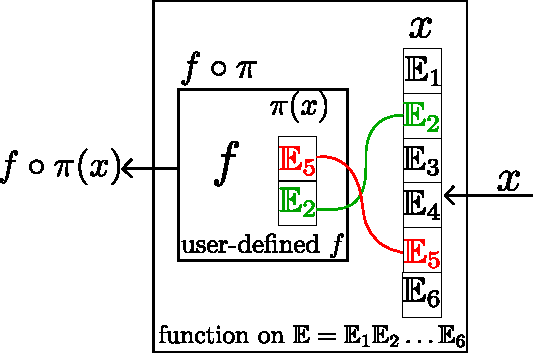
\includegraphics[width=.7\linewidth]{papers/Humanoids2015/figure/auto_mapping_text.pdf}
\caption{automatic variable mapping}
\label{fig:auto_map}
\end{figure}

\subsection{Problem Generator}

The problem generator is the tool constructing the optimization problem.
It registers all the variables and the functions related to a given problem.
Each function is likely to bring additional variables with it.
For each contact contributing to the balance, a variable on $\mathbb{R}^3$ representing the contact force is added to the problem.
The associated wrench is added to the stability constraints.
Once the registration is complete, the complete manifold of the problem is generated and uses the information of the Automatic mapping to ``plug" each function with the correct sub-manifold.
Subsequently, the optimization problem can be generated and passed to the solver.
The communication between the solver and the generated problem is made through the RobOptim framework\footnote{\url{http://www.roboptim.net/}}.% ~\cite{moulard:jsme:2013, moulard:jrsj:2014}.

\section{Problem formulations}
\label{sec:3}
Let $q=[q_F^T; q_r^T]\in\mathbb{R}^3\times SO(3)\times \mathcal{M}_r$ be the combination of the free-flyer of the robot $q_F\in \mathbb{R}^3 \times SO(3)$ and the articular parameters $q_r\in\mathcal{M}_r$.
Let $\mathcal{W}_i(p)=\{f_i,m_i(p)\}$ be the wrench (force+moment) applied by the environment onto the robot at contact $i$ and expressed on point $p$.
A frame $F$ is composed of a reference point and an orthonormal basis of 3 vectors $F = \{O, (x, y, z)\}$.

Here is a list of constraints that we consider in our problem (implementation of other ones is on-going):
\begin{itemize}
\item Joint limits ${q^-} \leq q_r \leq {q^+}$:\\
These cannot be directly translated on manifolds other than $\mathbb{R}^n$. For example, spherical joints can be parametrized on $S2 \times \mathbb{R}$, then the $S2$ part can be limited by a cone, and the $\mathbb{R}$ part can have real bounds. 
\item The contact constraint consists in identifying the features of two frames $F_1$ and $F_2$. For example, for a planar contact, we get the set of equation~\ref{eq:planar_contact}.

\begin{equation}
  \begin{split}
    (O_2-O_1).z_1 = 0\\
    z_2.z_1 \leq 0 \\
    z_2.x_1 = 0 \\
    z_2.y_1 = 0
  \end{split}
  \label{eq:planar_contact}
\end{equation}

Note that on $F_2$ only the point $O_2$ and the vector $z_2$ are necessary.
Other types of contacts can be created that way, by equalizing other features, as explained in \cite{escande:ras:2013}.

\item The stability constraint ensures that the Euler-Newton equation~(\ref{eq:NewtonWrench}) is balanced for the set of external wrenches applied to the robot (gravity $\mathcal{W}_G$ and contact forces $\mathcal{W}_i$).
  \begin{equation}
    \sum_{i}{\mathcal{W}_i(p)} + {\mathcal{W}_G(p)} = 0
    \label{eq:NewtonWrench}
  \end{equation}
  For each contact that bears forces ("stability" contact), a wrench applied on the robot at the contact point is added to the problem.
  That wrench is parametrized on a subset of $\mathbb{R}^6$ depending on the type of contact.
  For punctual contacts, the moment part is null on the application point.
  Only a parametrization of the force part on $\mathbb{R}^3$ is needed.
  We model planar contacts as a combination of punctual forces applied at each vertex of the contact polygon.
  In the case of interaction forces between 2 robots, only one wrench is created and it is used as is in the stability equation of one robot and its opposite is used for the stability of the second robot.

\item The friction cone constraint limits the tangential part of every forces to avoid slippage. We write it as~\ref{eq:friction} (with $\mu$ the friction coefficient)
\begin{equation}
  \begin{split}
    \mu^2f_z^2-f_x^2-f_y^2 \geq 0 \\
    f_z \geq 0
  \end{split}
  \label{eq:friction}
\end{equation}
\end{itemize}

The frame in which the constraints are written matters critically.
Most often, the frame's configuration depends on a part of the optimization variables, that must be accounted for in computing the constraints' Jacobian.
Our framework computes such dependencies automatically.

Our current PG (i.e. coding state) does not include yet collisions and auto-collisions, nor torque limits. Their implementation is on-going and is simply the matter of coding time.
Another important part is its cost function.
We only mention the cost function that have specificities when dealing with manifolds, the distance to a reference posture $q_0$.
On a robot that has all its articulations parametrized on $\mathbb{R}$ the distance can be expressed simply with the Euclidean norm $d = \norm{q_j-q_0}^2$.
Since we work on non-Euclidean manifolds, the logarithm function on the manifold must be used. It gives the distance vector between two points in the tangent space, the norm of this vector can be used as a distance.
So we get $d = \norm{\text{log}_{q_0}(q_r)}^2$.


%FROM HERE IT IS OLD TEXT

%There can be several kinds of contact between a surface of the robot and its environment(which could contain other robots).
%We denote $\mathcal{S}_R$ and $\mathcal{S}_E$ the two surfaces belonging to two bodies $\mathcal{B}_R$, $\mathcal{B}_E$ that are to be put in contact.
%We equip those surfaces with a frame $\mathcal{F} = \{O, (x, y, z)\}$, with $O$ a point of contact on the surface, and $z$ a vector normal to the surface at $O$.
%The transformation that leads from the reference frame of a body $\mathcal{B}$ to the reference frame of a surface $\mathcal{S}$ is denoted $^\mathcal{S}H_\mathcal{B}$.
%Note that those two surfaces do not need to be plane, a curved continous surface would suit as well.
%For a contact to be geometricaly satisfied, the planes defined by $\{O, (x, y)\}$ on both surfaces must be coplanar with normals of opposite directions.
%This can be assured by satisfying the following set of equation:

%\begin{align}
  %\begin{split}
  %(O_R-O_E) . z_E = 0 \\
  %z_R . x_E = 0 \\
  %z_R . y_E = 0 \\
  %z_R . z_E \leq 0
  %\end{split}
  %\label{eq:floating contact}
%\end{align}

%If any(either or both) of the two surfaces in contact is non-plane, finding the exact location of the contact point on the surface is necessary, because then, the normal to the contact is not known in advance.
%In that situation, we propose to paramaterize the contact frame on the surface on a 1 or 2-dimentional manifold.
%\begin{equation}
  %\mathcal{F}(u_S\in \mathcal{M}_S) = \{O(u_S), (x(u_S), y(u_S), z(u_S)\}
%\end{equation}
%Which, depending on the shape, could be $\mathbb{R}^2$ or $S2$.
%In that case, an additional set of variables $u_S\in \mathcal{M}_S$ is added to the optimization problem as well as the constraint set \ref{eq:floating contact} depending on it.

%The floating contact constraint can be extended to fix the contact to a given position and orientation by adding to it the following set of equation that locks the degrees of freedom of rotation around the normal and translation in the tangent plane of the contact:

%\begin{align}
  %\begin{split}
  %(O_R-O_E) . x_E = 0 \\
  %(O_R-O_E) . y_E = 0 \\
  %y_R . x_E = 0 \\
  %x_R . y_E = 0
  %\end{split}
  %\label{eq:fix planar contact}
%\end{align}

%Those two sets of equations \ref{eq:floating contact} and \ref{eq:fix planar contact} can easily be recombined to generate other types of constraints(e.g. fixing only the translation, or only the rotations...).

%For any scenario to be realistic, the robot must satisfy its stability constraint. Given a set of wrenches applied on the robot $\{\mathcal{W}_0, \mathcal{W}_1...,\mathcal{W}_{n_w}\}$.
%The sum of all those wrenches applied on a singular point must be zero.
%For each punctual contact that needs to bear forces, a new wrench is created, that wrench is parametrized by a set of two vectors describing its force $f = (f_x, f_y, f_z)^T \in \mathbb{R}^3$ and moment $m = (m_x, m_y, m_z)^T \in \mathbb{R}^3$ at the contact point.
%We denode $\mathcal{W}_G$ the wrench generated by the weight of the robot: $\mathcal{W}_G(CoM) = \{(0, 0, -mg)^T, (0, 0, 0)^T\}$. For any chosen reduction point $p$, the stability constraint writes as follows:

%\begin{equation}
  %\sum_{i=0}^{n_w}{\mathcal{W}_i(p)} + {\mathcal{W}_G(p)} = 0
  %\label{eq:NewtonWrench}
%\end{equation}

%Equation \ref{eq:NewtonWrench} can be rewritten with only vectors as:

%\begin{equation}
  %\begin{split}
  %\sum_{i=0}^{n_w}{f_i} - m g = 0 \\
  %\sum_{i=0}^{n_w}{m_i(p)} + {m_G(p)} = 0
  %\end{split}
  %\label{eq:NewtonForceMoment}
%\end{equation}

%A usual choice of reduction point for those equations is the center of mass of the robot. In which case the moment part of the gravity wrench is null.
%In the case of surfacic contact between two plane surfaces, the contact polygon is determined and a punctual force with zero moment is added on each vertex.
%The forces generated on each point need to satisfy the Coulomb friction cone equations which writes as follows for a friction coefficient $c$:

%\begin{equation}
  %\begin{split}
    %c^2 f_z^2 - f_x^2 - f_y^2 \geq 0 \\
    %f_z \geq 0
  %\end{split}
  %\label{eq:FrictionCone}
%\end{equation}

%It is not straightforward to devise a friction limit in terms of moment.
%Which is why, in the current study, we considere that the punctual contacts are perfect and do not generate moment on their application point.
%This translates in fixing the moment variables of the wrench to zero while the force variables still exist.
%In the case of planar contacts, of course, the moment part cannot be ignored.
%But, given a planar polygon in which the contact happens, the wrench generated by this contact can be modeled as a set of punctual forces, one on each vertex of the polygon. Which respect the same friction cone equations \ref{eq:FrictionCone} and are taken into account in \ref{eq:NewtonWrench}.

\section{Simulation Results}
\label{sec:4}
Here, we present several posture generation problems resolution that leverage the specific capabilities of our software.

\begin{figure*}
\centering
  \centering
  \setlength\fboxsep{0pt}
  \setlength\fboxrule{1pt}
  \fbox{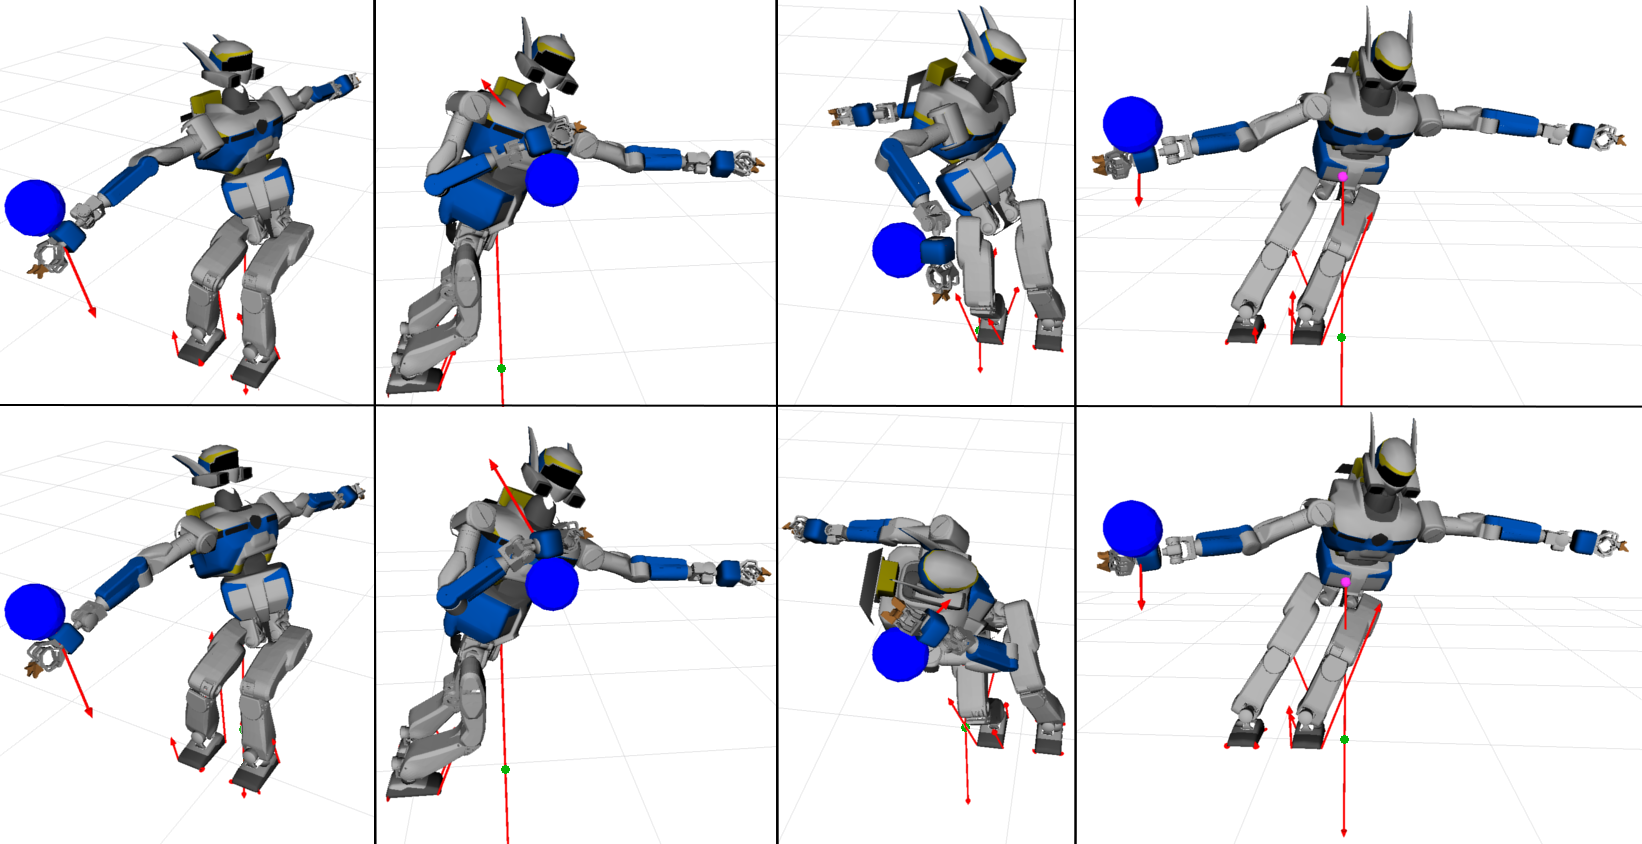
\includegraphics[width=\textwidth]{papers/Humanoids2015/figure/4directionsStrokesWithCoM.png}}
  %\fbox{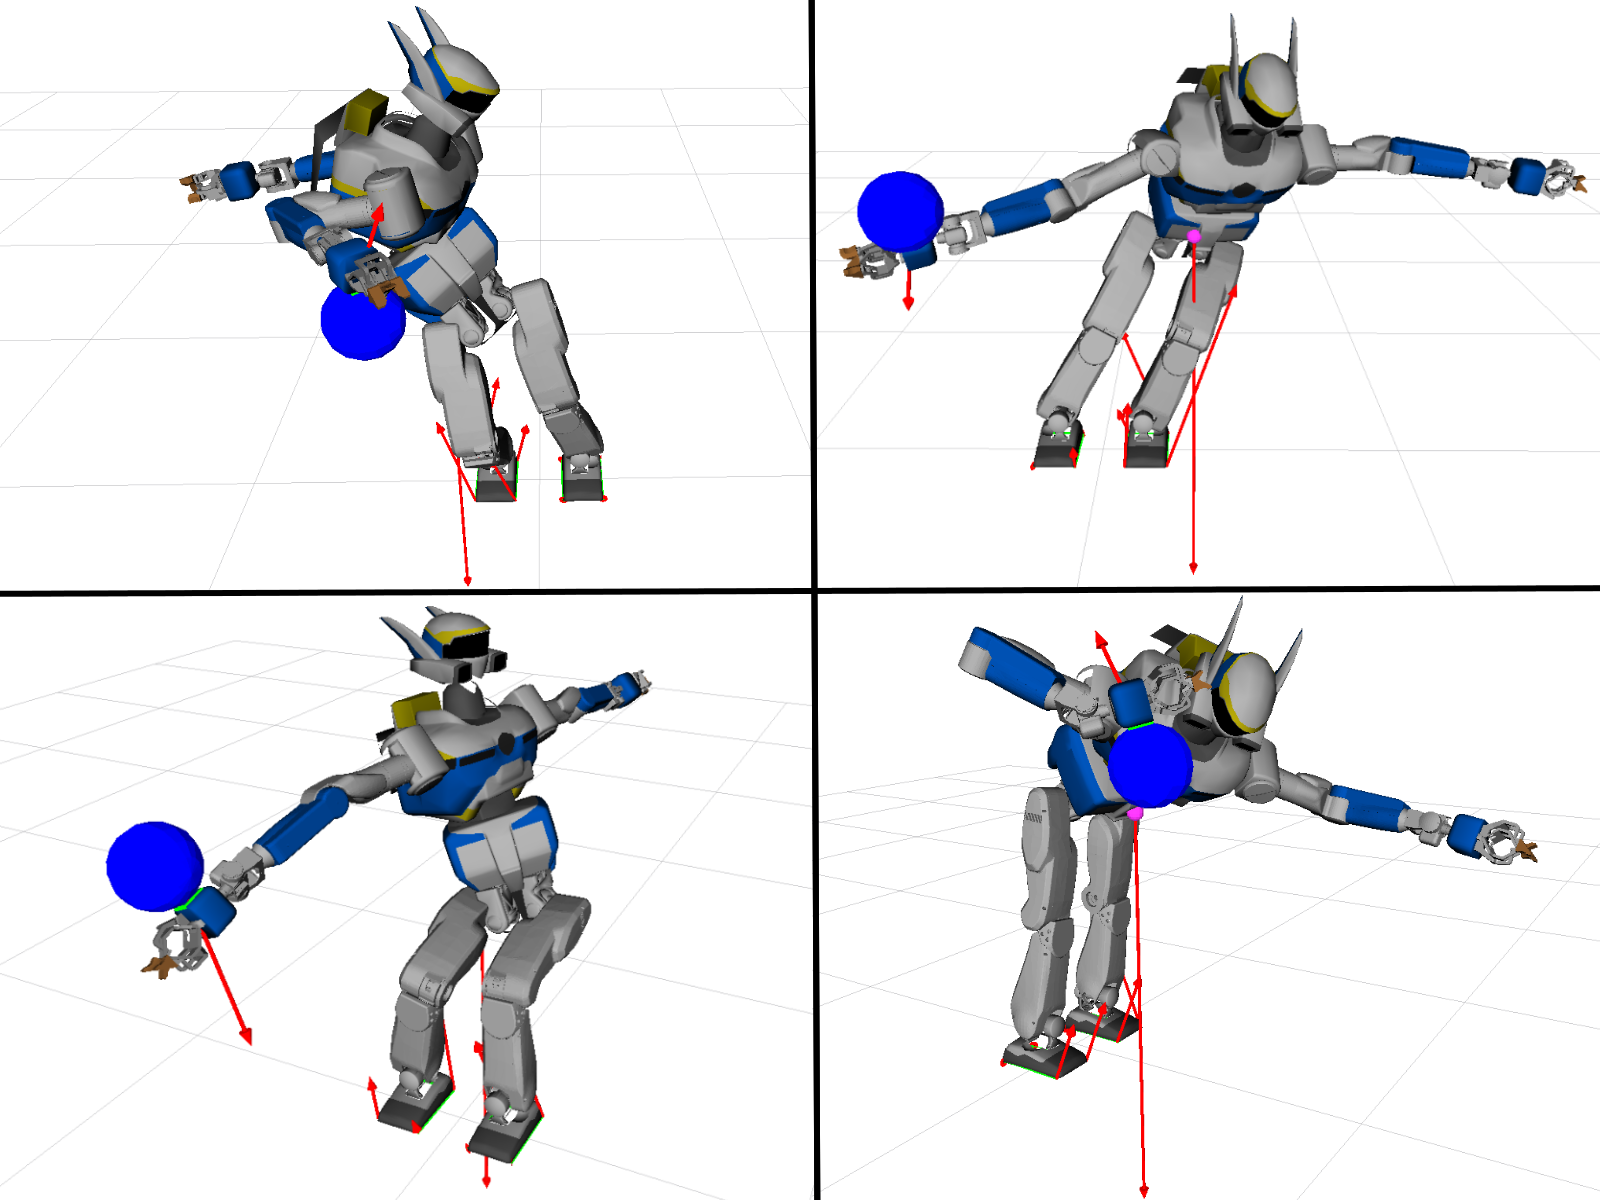
\includegraphics[width=.95\linewidth]{papers/Humanoids2015/figure/contact_plan_sphere_4_directions.png}}}
  \caption{HRP2-Kai leaning on sphere with right wrist to point the left gripper as far as possible in 4 cardinal directions. Top row: semi-predefined contact; Bottom row: free contact with parametrized wrist. Projection of the CoM on the ground (green dots)}
\label{fig:contact_plan_sphere}
\end{figure*}

\subsection{Application to plan-sphere contact}
When we consider a planar contact, having a frame $F_{S}$ fixed in reference to $F_{B}$ is sufficient because the equations describing that contact are invariant w.r.t. the point's location.
But for different contact topologies, the location of the contact point in the body's frame $F_{B}$ matters.
We propose to parametrize the location and normal of the contact point with an additional variable.

We consider the contact between a body's flat surface $S_B$ of normal $n_B$, with the surface of a sphere $S_s$ of center $c_s$, radius $r_s$, and let $p_s$ and $n_s$ be a point and its normal to $S_S$.
The most general way to express such a constraint is to ensure that $p_s$ is on $S_B$ and that $n_s$ and $n_B$ are opposite.
This means creating a variable $v_{S2}$ on the manifold $S2$ and map $p_S$ and $n_S$ on it.
In our framework, this constraint is expressed exactly as the contact between 2 planar surfaces, once the mappings of $p_s(v_{S2})$ and $n_s(v_{S2})$ are done.
In a framework that does not handle manifolds (as we do), it would require to setup a specific constraint, ensuring that the distance between $c_s$ and $S_B$ is equal to $r_S$.

In Fig.~\ref{fig:contact_plan_sphere} we show the results obtained by solving a problem where the HRP2-Kai robot has to keep its feet in contact with the ground at fixed positions, touch a sphere with a side of its right wrist and point as far as possible in a given direction $d$ with its left hand, under balance constraints.
The top row of Fig.~\ref{fig:contact_plan_sphere} shows the results for this problem with several different $d$.
%It shows that our optimization algorithm finds an optimal contact point on the sphere to reach its goal as best as possible while satisfying the given constraints.
In every situation, the projection of the CoM is outside the polygon of support, meaning that such postures would not be reached without leaning on the sphere.

\subsection{Contact with parametrized wrist}

\begin{figure}[!htb]
\centering
  \centering
  \setlength\fboxsep{0pt}
  \setlength\fboxrule{1pt}
  \fbox{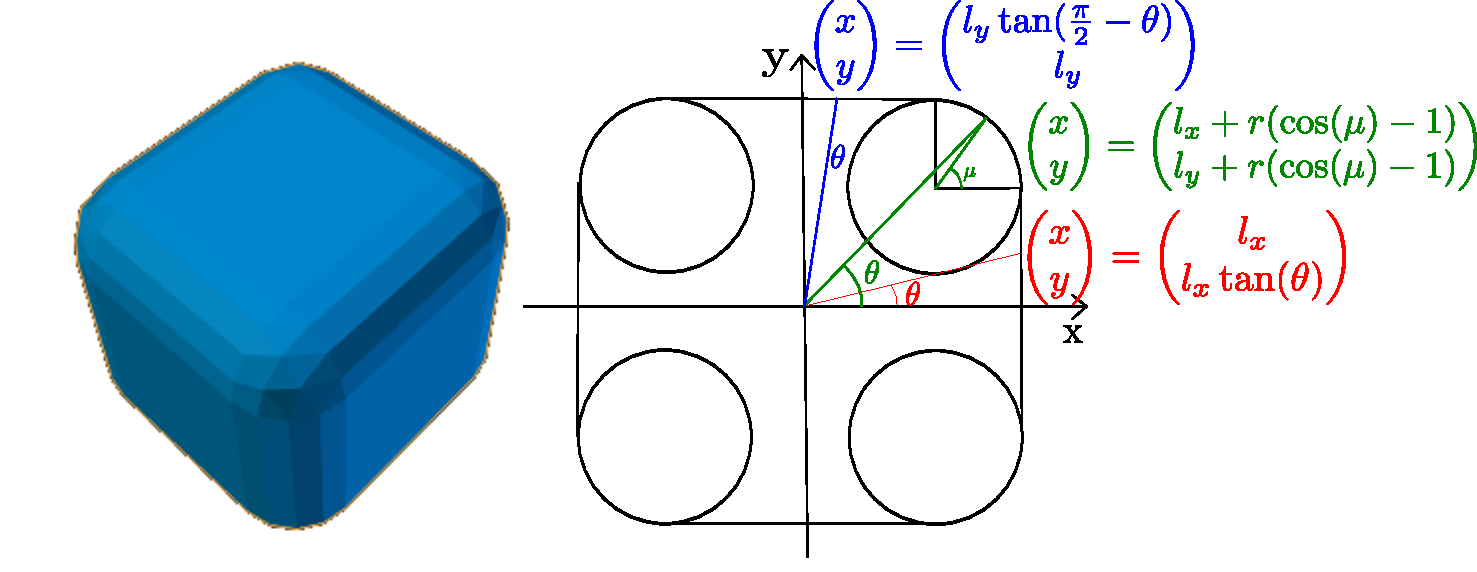
\includegraphics[width=.95\linewidth]{papers/Humanoids2015/figure/param_wrist_detail.pdf}}
	%\fbox{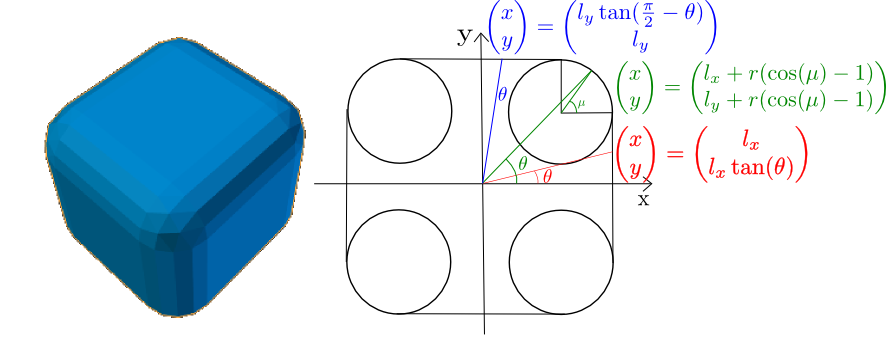
\includegraphics[width=.95\linewidth]{papers/Humanoids2015/figure/param_wrist_detail.png}}
\caption{Parametrization of the wrist of HRP2-Kai}
\label{fig:param_wrist_detail}
\end{figure}

Being able to choose the location of the contact point on the sphere is interesting, but a limitation of this formulation is that the contact point on the wrist of the robot is restricted to one single user-defined face.
Instead, we describe the shape of the wrist body as a parametric function and let the contact point on the wrist as well as its counterpart on the sphere, result from the optimization process.
The section of HRP2-Kai's wrist is a square with rounded edges.
We parametrize this shape as shown in Fig.~\ref{fig:param_wrist_detail}:
we consider the angular coordinate $\theta$ of the point on the section. It is added as a variable to the problem.
The shape of a quarter of section $[0;\pi/2]$ is a succession of a vertical line, a quarter of circle and a horizontal line.
This pattern is repeated for the 3 other quarters.
The equations are given in Fig.~\ref{fig:param_wrist_detail}.
In our framework, we define the function describing the shape of the wrist, create a frame parametrized by that function and then define the contact between that frame and the point and normal on the sphere.
This formulation not only is very easy to implement, but most importantly, allows for richer posture generations.
The optimization algorithm chooses the contact point on the sphere as well as the contact point on the wrist, which leads to a wider accessibility range, and a better satisfaction of the cost function.
The bottom row of Fig.~\ref{fig:contact_plan_sphere} displays the results of this simulation for the robot pointing in 4 directions.
Notice that on the 2nd and the 4th (pointing forward and to the left) images, the results for the 2 types of models are nearly identical.
Whereas in the 1st and 3rd images, different faces of the wrist have been chosen(On the 1st, the wrist is rotated by $180^{\circ}$, and $90^{\circ}$) on the 3rd).
In these 4 cases, the contact with parametrized wrist gives a better cost of the objective function.
This observation scales:
we solved this problem for 5000 random pointing directions, and in average, the contact with parametrized wrist allows to reach 5mm further.
The success rate of the solver is $98.5\%$ in the parametrized wrist case against $99.9\%$ when the face is fixed. The numbers of iterations are similar.

%Also, that kind of formulation makes it easier for the user to generate satisfactory postures, as he does not need to specify the plan contact surface anymore.
This method is certainly scalable, and can be used for any kind of humanoid robot and environment.
Yet, it requires to have a parametric equation of the surface.
We plan to implement a method to generate a parametrized surface point and its normal directly from the 3D mesh of an object.
The accompanying video shows the optimization process for the problem with parametrized wrist. Notice on the video that the contact point on the wrist changes sides all along the iterations.

\subsection{Contact with an object parametrized on $S2$}

In this simulation case, we want the HRP-4 robot (anther model) to carry a cube with its two hands.
The most general way to do it is to select a face of the cube for each contact, and enforce the contact between that face and the hand's surface.
We propose to approximate the cube with a superellipsoid and to parametrize the resulting shape on $S2$.
The implicit equation of a superellipsoid is $S(x,y,z) = 0$, with
\begin{equation}
  S(x,y,z) = \left( \left|\frac{x}{A}\right|^r + \left|\frac{y}{B}\right|^r\right)^\frac{t}{r} + \left|\frac{z}{C}\right|^t - 1
  \label{eq:super_ellipsoid}
\end{equation}

A point in $S2$ is represented by a vector $v=(x,y,z)$ in $\mathbb{E} = \mathbb{R}^3$. To a given unit vector $v$ we associate a point $\alpha v$ on the surface of the superellipsoid by solving $S(\alpha v) = 0$ for $\alpha$. At this point, the normal is given by $\dfrac{\nabla S(\alpha v)}{\left\|\nabla S(\alpha v)\right\|}$ which simplifies into $\dfrac{\nabla S(v)}{\left\|\nabla S(v)\right\|}$.
%It returns the intersection between any unit vector and the surface of the super ellipsoid.
%Also we generate a similar function that returns the normal of the intersection point.
Given this parametrization, we write a contact constraint between the frame of the hand of the robot and the point and normal on the surface of the superellipsoid.

In Fig.~\ref{fig:hrp4_cube} we present some results for a posture generation problem with manipulation: On the left side, the feet are free to move on a sphere, and, on the right side, the left foot position is fixed and the right foot is free to move on the ground. The hands must be in contact with the cube. The cube is free to move (parametrized by $\mathbb{R}^3 \times SO(3)$) and has it own set of Euler-Newton equations, which must be fulfilled.
On the accompanying video, one can observe how the contact points on the cube evolve along with the optimization.
%For each contact with the cube, a variable on $S2$ is added to the problem to parametrize the contact point.
%Each hand is in contact with a point and normal on the cube.

%\begin{figure}
%\centering
  %\centering
  %\setlength\fboxsep{0pt}
  %\setlength\fboxrule{1pt}
  %\fbox{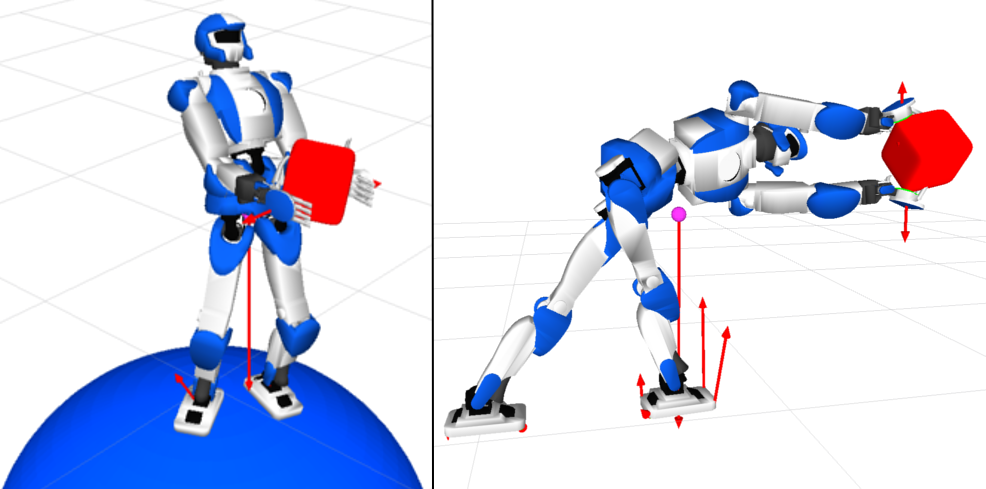
\includegraphics[width=.99\linewidth]{papers/Humanoids2015/figure/hrp4CubeOnSphere.png}}
%\caption{HRP4 carrying 2kg a cube. Left: the objective function is to maintain the cube at a given position. Right: it is to put the cube as far as possible in a given direction}
%\label{fig:hrp4_cube}
%\end{figure}

\subsection{Posture Generation with a human model}

\begin{figure}
\centering
  \centering
  \setlength\fboxsep{0pt}
  \setlength\fboxrule{1pt}
  \fbox{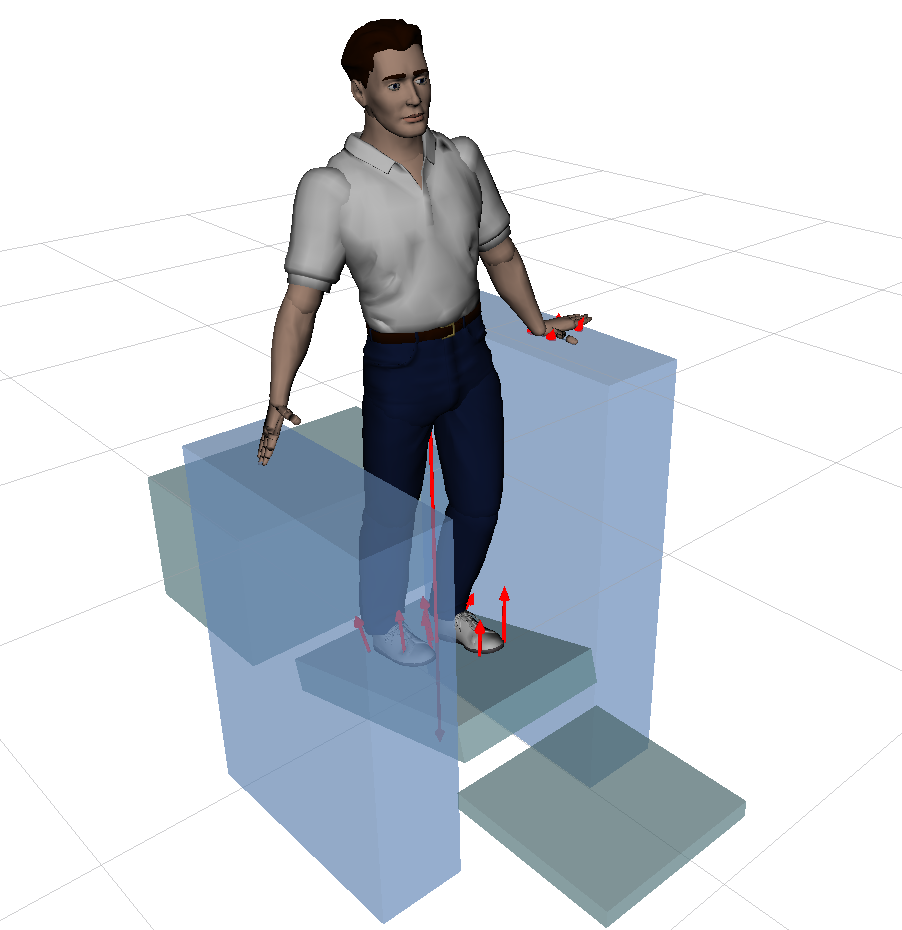
\includegraphics[width=.7\linewidth]{papers/Humanoids2015/figure/cropped_human.png}}
\caption{Posture generation for a human avatar}
\label{fig:pg_human}
\end{figure}

The geometric model of a human is much more complex than the one of a humanoid robot in terms of topology.
Even with the simplest models, the shoulders, wrists, ankles, or hips need to be described as spherical joints, and therefore be parameterized on $SO(3)$.
We showcase that our solver is able to handle such complex models as a human avatar in Fig.~\ref{fig:pg_human}.
Our human model has spherical joints on its wrists, shoulders, torso, hips and ankles.
With the addition to the free-flyer, the manifold that contains the articular space of that human model is:
$\mathcal{M}_H = SO(3)\times\mathbb{R}^3\times \left(SO(3)\right)^9\times\mathbb{R}^4$.
We fixed the neck's joints as well as the fingers to avoid unnecessary variables.
In this simulation, we require the human to stand on an inclined slope while leaning on the left side's wall.
Since we have not yet implemented the boundary limits on spherical joints, the model could reach non desired configurations.
That issue limits for the time being the number of scenarios that we can solve.
But the use of a cost function on the posture of type $d = \norm{\text{log}_{q_0}(q_j)}^2$, attracting the avatar to a basic standing posture, allowed us to have acceptable results.

\section{Discussion and conclusion}
\label{sec:Conclusion}
Writing the posture generation problem as a non-linear optimization problem on non-Euclidean manifolds proves to be an elegant approach in terms of code structuring and user interface, in addition to mathematical readability. This work is still on-going and only preliminary results of the current state of the implementation are shown. We illustrate some posture generation problems with the HRP2-Kai and the HRP-4 humanoid robots; the results are very promising indeed. Our future (on-going) work is focused on the following streams:
\begin{itemize}
\item complement other functionalities as ready-to-use templates (e.g. constraints on task forces, collision avoidance, etc.);
\item specialize the solver to humanoid PG problems and benchmark various numerical approaches (e.g. for the choice of the Hessian approximation, the trust region, tuning some parameters, etc.) and exploiting, if any, robotic model properties;
\item improve convergence, numerical robustness and computation time of the PG. Currently, the resolution of any of the presented problems takes a few seconds on a laptop with Intel Core i7-3840QM CPU @ 2.80GHz. We aim at reducing it to a tenth of a second.
\end{itemize} 
Once the code is more stable and finalized, we plan to make it open-source.

%\chapter{
New Porsture Generation
}

\section{List of contributions}
\begin{itemize}
  \item{Posture Generation, variables and architecture}
    \begin{itemize}
      \item Geometric expressions:
        \begin{itemize}
          \item Represent everything based on frames
          \item Automatic derivative computation
        \end{itemize}
      \item Automatic mapping
      \item Problem generator: a posture generation problem factory
    \end{itemize}
  \item{Problem Formulation: formulation of usual problems in the geometric expressions framework}
    \begin{itemize}
      \item Contact with plane surface
      \item Static equilibrium: Newton/CoM projection
      \item Forces in friction cones
      \item Articular limits
      \item Torque limits
      \item Torque minimization
      \item Goal Posture
    \end{itemize}
  \item{Implementation of new types of constraints in our formulation}
    \begin{itemize}
      \item Contact with parametrized surfaces on Rn
      \item Contact with parametrized surfaces on S2: Sphere, SuperEllipsoid
      \item Contact with Catmull-Clark Subdivision surfaces
    \end{itemize}
  \item{Simulation Results}
\end{itemize}

%\chapter{
  Forces in Posture Generation
}

\section{List of contributions}
\begin{itemize}
  \item{Contact with desired force}
  \item{Potential contacts}
\end{itemize}

%\chapter{
  Evaluation of the PG, experimentaion
}

\section{List of contributions}
\begin{itemize}
  \item Understanding the environment through a point-cloud
    Extraction of plane polygons from Kinect acquired point-clouds.

    Segmentation pipeline:
    \begin{itemize}
      \item Acquisition
      \item Filtering
      \item Region growing segmentation
      \item Planar Extraction
      \item Planar projection and Hull convex generation
      \item Re-orientation and transfer to the planner
    \end{itemize}
  \item Generation of sequences of postures on segmented environment
  \item{Simulated scenarios planned on real-environment: HRP-2 climbing on table through stairs, HRP-2 climbing on table through slope}
  \item{Optimization of the solvers parameter for a class of problems}
    \begin{itemize}
      \item Developpement of a list of typical robotics optimization problem
      \item Training of a genetic algorithm to find the "best" solver tuning to solve our list of problems
    \end{itemize}
  \item{Several scenarios, including Airbus}
\end{itemize}




% ********************************** Back Matter *******************************
% Backmatter should be commented out, if you are using appendices after References
%\backmatter

% ********************************** Bibliography ******************************
\begin{spacing}{0.9}

% To use the conventional natbib style referencing
% Bibliography style previews: http://nodonn.tipido.net/bibstyle.php
% Reference styles: http://sites.stat.psu.edu/~surajit/present/bib.htm

\bibliographystyle{apalike}
%\bibliographystyle{unsrt} % Use for unsorted references  
%\bibliographystyle{plainnat} % use this to have URLs listed in References
\cleardoublepage
\bibliography{References/SBbib} % Path to your References.bib file


% If you would like to use BibLaTeX for your references, pass `custombib' as
% an option in the document class. The location of 'reference.bib' should be
% specified in the preamble.tex file in the custombib section.
% Comment out the lines related to natbib above and uncomment the following line.

%\printbibliography[heading=bibintoc, title={References}]


\end{spacing}

% ********************************** Appendices ********************************

\begin{appendices} % Using appendices environment for more functunality

%
%%%%%%%%%%%%%%%%%%%%%%%%%%%%%%%%%%%%%%%%%%%%%%%%%%%%%%%%%%%%%%%%%%%%%%%
%                          Thesis Appendix A                          %
%                       Numerical Optimization                        %
%%%%%%%%%%%%%%%%%%%%%%%%%%%%%%%%%%%%%%%%%%%%%%%%%%%%%%%%%%%%%%%%%%%%%%%

\chapter{Numerical Optimization: Introduction}
\label{chapter:optimization}

\nomenclature[x-R]{$\mathbb{R}$}{Real space}
\nomenclature[x-R+]{$\mathbb{R}_\geq0$}{The set of positive Reals}
\nomenclature[x-S]{$\mathit{S}$}{Variable space}
\nomenclature[x-M]{$\mathcal{M}$}{A Manifold}
\nomenclature[x-T]{$T_x\mathcal{M}$}{The tangent space of manifold $\mathcal{M}$ at point x}
\nomenclature[a-F]{$F$}{The set of linearized feasible directions}
\nomenclature[a-f]{$f$}{Objective function}
\nomenclature[a-c]{$c_i$}{Constraint function}
\nomenclature[a-x]{$x$}{Optimization variable}
\nomenclature[a-xstar]{$x^*$}{Solution of the optimization problem}
\nomenclature[a-E]{${E}$}{Set of index for which constraints are equality constraints}
\nomenclature[a-I]{${I}$}{Set of index for which constraints are inequality constraints}
\nomenclature[x-L]{$\mathcal{L}(x,\lambda)$}{Lagrangian function of the optimization problem}
\nomenclature[G-o]{$\Omega$}{Feasible set}
\nomenclature[z-st]{s.t.}{subject to}
\nomenclature[z-KKT]{KKT}{Karush-Kuhn-Tucker first order optimality conditions}
\nomenclature[z-LICQ]{LICQ}{Linear Independence Constraints' Qualification}
\nomenclature[z-QP]{QP}{Quadratic Programming}
\nomenclature[z-IQP]{IQP}{Inequality constrained Quadratic Programming}

\graphicspath{{Appendix1-Optim/Figs/}}

%{{{SECTION: LIST OF CONTRIBUTIONS
%\section{List of contributions}
%\begin{itemize}
  %\item \sout{Introduction to optimization}
  %\item \sout{Notions of unconstrained optimization}
  %\item \sout{Notions of Constrained Optimization}
  %\item \sout{KKT}
  %\item Line Search
  %\item Trust Region
  %\item Filter
  %\item Merit function
  %\item SQP
  %\item Restoration phase
  %\item \sout{Hessian Approximation: BFGS, SR1}
%\end{itemize}
%}}}
\section{Introduction}
In modern science, optimization has an important place.
Mechanical engineers optimize the shape of structural parts.
Investors optimize the profit of a portfolio while minimizing the risks of loss.
Chemists optimize the efficiency and speed of reactions.
When it comes to robotics, optimization is widely used.
From the design of a robot to its actuation.
Any positioning of a robot requires the computation of the articular parameters of each joint of the robot, finding such parameters might be possible by using analytical methods for simple robots, but for robots as complex as humanoid robots, it is not possible.
Most often, an optimization process is used.

The goal of an optimization algorithm is to find an optimal solution $x^*$ to a problem.
Optimal in the sense that the solution is an optimum of a given objective function $f$.
And solution of a problem in the sense that it satisfies a set of $m$ constraints $\{c_i,\ i\in [1,m]\}$.
Both the constraints and the objective function are defined on the variable space $\mathit{S}$, which is the space in which the variable $x$ lives and in which we search a solution $x^*$ to our problem.

In order to present the principles of optimization, in this chapter, we will always consider that the variable space is $\mathit{S}=\mathbb{R}^n$.
We first consider unconstrained problems.
That type of problem will not be used in the rest of our dissertation, therefore, we will just present them shortly.
We will then focus on constrained optimization problems and the numerous methods used in their resolution.
We will particularly detail one specific constrained problem resolution algorithm that is the Sequential Quadratic Program (SQP).
The extension of those methods to solving problems on more complex variable spaces that are the non-Euclidean manifolds is the topic of Chapter~\ref{chapter:optimization_on_noneuclidean_manifolds}.

This Appendix does not pretend to give a fully detailed overview of numerical optimization methods, it gives the reader a quick overview of some key principles.
For more detailed information, we invite the reader to refer to the excellent books that we took inspiration from to write this chapter~\cite{nocedal:book:2006, bonnans:book:2003, boyd2004convex}.

\section{Unconstrained Optimization}

An unconstrained optimization problem consists of an objective function to minimize, without any constraint.
This problem, denoted $\mathcal{P}$, can be formulated as follows:

\begin{equation}
  \minimize_{x\in\mathbb{R}^n}\ {f(x)}
\label{eq:unconstrainedOptim}
\end{equation}

The classical approach to solve $\mathcal{P}$ is to use an iterative algorithm, starting from an initial guess $x_0$, and converging toward the solution $x^*$.
A very basic optimization scheme is presented in Algorithm~\ref{alg:basic_optim}.

\begin{algorithm}
\begin{algorithmic}
  \State{Starting from an initial guess $x_0$}
  \While{Convergence condition not met}
  \State{Compute descent direction $p_k$}
  \State{Update $x_{k+1}\leftarrow x_k + p_k$}
  \EndWhile{}
  \caption{Basic optimization scheme}
\label{alg:basic_optim}
\end{algorithmic}
\end{algorithm}

The objective function is not necessarily completely known, in the sense that we cannot always have an explicit formula. Often, the function $f$ is computed by another program that is able to compute $f(x)$, $\nabla_x f(x)$ and sometimes $\nabla_{xx} f(x)$ for a given value of $x$.
In order to have an efficient algorithm, we need to avoid any unnecessary computation of $f(x)$ and its derivatives.
We denote the values taken by $x$ along the iterations as $x_0$, $x_1$, $x_2$,\ldots $x_i$.
And $f(x_i)$ is denoted $f_i$.

Since our knowledge of the objective function is only partial, without further assumptions, it is not possible to guarantee that a point $x^*$ is a global solution:

\begin{equation}
  \text{$x^*$ is a global solution of $\mathcal{P}$ on $\mathit{S}$ } \equiv \forall x \in \mathit{S}, f(x^*) \leq f(x)
\end{equation}

Though, we can find a local solution $x^*$ of $\mathcal{P}$ (a local minimizer of $f$): such that there exist a neighborhood $\mathit{N}$ of $x^*$ where $\forall x\in \mathit{N}$, $f(x^*) \leq f(x)$.
Or even a strict local minimizer of $f$: such that there exist a neighborhood $\mathit{N}$ of $x^*$ where $\forall x\in \mathit{N}$, $f(x^*) < f(x)$.
That is the kind of solution that we are looking for and that our algorithms should find.

Under the assumption that the objective function is smooth and sufficiently continuous ($\mathcal{C}^2$), we have the following sufficient conditions for the optimality of $x^*$:

\begin{theorem}
  If $\nabla^2f$ is continuous in an open neighborhood of $x^*$, $\nabla f(x^*)=0$ and $\nabla^2 f(x^*)$ is positive definite.
  Then $x^*$ is a strict local minimizer of $f$.
\label{optimalityTheorem}
\end{theorem}

The same definition can be given for a local minimizer with $\nabla^2f(x^*)$ positive semi-definite.

There are several ways to choose a descent direction $p_k$ from an iterate $x_k$. The
most obvious one is probably the steepest descent direction $-\nabla f_k$. This
method provides the direction along which f decreases most rapidly and only
requires the evaluation of the first derivative of $f$, but that method can
become extremely slow on complicated problems. Another popular approach is the
Newton method, in which the objective function is approximated to the second
order

\begin{equation}
  f(x_k+p) = f_k + p^T\nabla f_k + p^T\nabla^2f_k p
\end{equation}

Then the chosen descent direction is the optimum of that approximated function,
the Newton direction.
\begin{equation}
  p^N_k = -{(\nabla^2 f_k)}^{-1} \nabla f_k
\end{equation}
The choice of this descent direction implies that the $\nabla^2f_k$ is positive
definite, in which case an adaptation of the definition of $p_k$ is required. Or
an approximation $B_k$ of $\nabla^2f_k$ that guarantees definite positiveness can be
used. %For example, the symmetric-rank-one (SR1) formula and the BFGS (Broyden,
%Fletcher, Goldfarb, Shanno) formula. Then the step becomes

\begin{equation}
  p_k = -B_k^{-1}\nabla f_k
\end{equation}

$p_k$ is then added to $x_k$ to compute $x_{k+1} \leftarrow x_k + p_k$ and the process is repeated until convergence is reached.

Many methods and refinements exist to solve this problem and some are presented in~\cite{nocedal:book:2006}.
Our main focus here is on methods to solve constrained problem as they arise in robotics.

%\subsection{Globalization methods (Section NEEDS TO BE REWRITTEN)}

%During the resolution of an optimization problem, the algorithm will generate a
%sequence of iterates $x_k$ starting from the initial iterate $x_0$ (Which is
%usually provided by the user). During the step $k$ of the optimization process,
%the solver, the current point is $x_k$ and we try to find $x_{k+1}$ such that
%$f(x_{k+1}) < f(x_k)$. There are several strategies to do that but we will only focus
%on 2 of them that are the most popular, the line-search and trust-region
%methods.

%\subsubsection{The Line-Search Strategy}
%In the Line-Search strategy, given a point $x_k$, a descent direction $p_k$ from this
%point is chosen and then a length of step is calculated to minimize the
%following 1-dimensional problem:
%\begin{align}
  %\minimize_{\alpha \in \mathbb{R}^+} f(x_k + \alpha.p_k)
%\label{eq:lineSearchNLP}
%\end{align}

%Once the best value of $\alpha$ has been found, the next iterate is computed:
%$x_{k+1} = x_{k} + \alpha p_k$ and the same process is repeated until a
%satisfying solution is found.

%It is not always necessary to find the optimal value of $\alpha$, especially if
%that is expensive. Indeed, $\alpha$ is only used to calculate the next iterate,
%from which another $p_k$ and $\alpha$ will be calculated. And in the end, the
%imprecision on the computation of $\alpha$ will be erased in the other steps of
%the resolution.

%There are several ways to choose a descent direction from an iterate $x_k$. The
%most obvious one is probably the steepest descent direction $-\nabla f_k$. This
%method provides the direction along which f decreases most rapidly and only
%requires the evaluation of the first derivative of $f$, but that method can
%become extremely slow on complicated problems. Another popular approach is the
%Newton method, in which the objective function is approximated to the second
%order

%\begin{equation}
  %f(x_k+p) = f_k + p^T\nabla f_k + p^T\nabla^2f_k p
%\end{equation}

%Then the chosen descent direction is the optimum of that approximated function,
%the Newton direction.
%\begin{equation}
  %p^N_k = -{(\nabla^2 f_k)}^{-1} \nabla f_k
%\end{equation}
%The choice of this descent direction implies that the $\nabla^2f_k$ is positive
%definite, in which case an adaptation of the definition of $p_k$ is required. Or
%an approximation $B_k$ of $\nabla^2f_k$ that guaranties definite positiveness can be
%used. For example, the symmetric-rank-one (SR1) formula and the BFGS (Broyden,
%Fletcher, Goldfarb, Shanno) formula. Then the step becomes

%\begin{equation}
  %p_k = -B_k^{-1}\nabla f_k
%\end{equation}

%\subsubsection{The Trust-Region Strategy}
%\label{ssec:the_trust_region_strategy}
%The Trust-Region Strategy works in an opposite way than the line-search one in
%the sense that during a line-search step, a direction is chosen, and based on
%that direction, a step-length is chosen. Whereas with a Trust-Region approach, a
%maximum step-length is chosen, and based on it, the descent direction and length
%are chosen.
%The principle of the trust region is that along the optimization process, a
%model of the problem is constructed and enriched at every step and at each step,
%the next iterate is the optimum of the model, with the constraint that the step
%to get there lies inside the trust-region. For example, let us consider that
%the trust region is a sphere of center $x_k$ and radius $\rho_k$, then the
%constraint on $p_k$ is $\|p_k\| \leq \rho_k$. A usual model to take for the
%objective function is the quadratic model with approximated Hessian
%\begin{equation}
  %m_k(p) = f(x_k+p) = f_k + p^T \nabla f_k + p^T B_k p
%\end{equation}
%And the optimization problem to solve at each step of the optimization is

%\begin{align}
  %\minimize_{p} & \quad f_k + p^T \nabla f_k + p^T B_k p \nonumber\\
%\text{s.t.}&
%\quad \|p\| \leq \rho_k
%\label{eq:trustRegionNLP}
%\end{align}

%Once the solution $p_k$ to this quadratic problem is found, its quality is
%estimated by evaluating the value of $f(x_k+p_k)$. If the actual decrease of $f$
%is satisfying (compared to the decrease predicted by the model) then the step is
%accepted and the size of the trust-region can be increased. Otherwise, the step
%is refused, the trust-region radius is reduced and a new step from $x_k$ is
%computed on that smaller trust region.

\section{Constrained Optimization}

Solving a constrained optimization problem consists in minimizing a cost function while satisfying a set of constraints.

A general formulation for such problems (that we denote $\mathcal{P}$) is:

\begin{equation}
  \label{formulation_NLCP}
  \mathcal{P} \equiv
  \left\{
  \begin{array}{l}
    \minimize\limits_{x\in\mathbb{R}^n}{f(x)}\\
    \text{ s.t. }
    \left\{
    \begin{array}{l}
      c_i(x) = 0,\ \forall i\in{E}\\
      c_i(x) \geq 0,\ \forall i\in{I}\\
    \end{array}
    \right.
  \end{array}
  \right.
\end{equation}

Where $f$ and $c_i$ are real-valued functions on a subset of $\mathbb{R}^n$.
$f$ is the objective function, and the $c_i$ are the constraint functions.
${I}$ and ${E}$ are sets of index such that $c_i,\ i\in{E}$ are the equality constraints, and $c_i,\ i\in{I}$ are the inequality constraints.

We define the feasible set $\Omega$ that contains all the feasible points (points satisfying the constraints) of $\mathcal{P}$.

\begin{equation}
  \Omega = \left\{ x\in \mathbb{R}^n:\ \forall i\in {E},\ c_i=0,\ \forall i\in{I},\ c_i \geq0\right\}
\end{equation}

The formulation~\ref{formulation_NLCP} can then be rewritten as:
\begin{equation}
  \label{formulation_NLCP_compact}
  \mathcal{P} \equiv \minimize_{x\in\Omega}{f(x)}
\end{equation}

In the general case, the problem~\ref{formulation_NLCP_compact} has multiple local solutions.
And finding the global minimizer of $f$ in $\Omega$ is a difficult problem that we do not treat in this thesis.
Our goal is to find a local minimizer $x^*$ of $f$ in $\Omega$.

\subsection{Optimality conditions}
\label{sub:optimality_conditions}

\paragraph{First-Order Optimality Conditions}

The First Order Optimality Condition (Karush-Kuhn-Tucker Condition) is a necessary condition verified by all solutions of problem~\ref{formulation_NLCP}.

We introduce the Lagrangian function of~\ref{formulation_NLCP}:
\begin{equation}
  \mathcal{L}(x,\lambda) = f(x) + \sum_{i\in E\cup I}\lambda_i c_i(x)
\end{equation}

Any given constraint $c_i$ is said to be active at $x$ if $c_i(x)=0$.
In particular, for any feasible point $x$, all equality constraints $c_i,\ i\in E$ are active.
An inequality constraint $c_i,\ i\in I$ is inactive if $c_i(x)>0$ and active if $c_i(x) = 0$

\begin{definition}
\label{active_set}
  The active set $\mathit{A}(x)$ at a feasible point $x$ is the set of all the indexes of active constraint.
  \begin{equation}
    \mathit{A}(x)=E\cup\{i\in I: c_i(x) = 0\}
  \end{equation}
\end{definition}

Most optimization algorithms make the assumption that at the solution, the constraints satisfy the following Linear Independence Constraints' Qualification (LICQ) definition:

\begin{definition}
  Given a point $x$ and an active set $\mathit{A}(x)$, we say that the LICQ holds if the set of active constraint gradient $\{\nabla c_i(x),\ i\in \mathit{A}(x)\}$ is linearly independent
\end{definition}

In general, if LICQ holds, none of the active constraints gradients can be zero.
%In particular, if any gradient of a constraint is null, then the LICQ does not hold.
%The LICQ should be taken into account during the formulation of a problem.

\begin{theorem}{First-Order Necessary Conditions}\\
\label{KKT_conditions}
  Suppose that $x^*$ is a local solution of~\ref{formulation_NLCP}, that the functions $f$ and $c_i$ are continuously differentiable, and that the LICQ holds at $x^*$.
  Then there is a Lagrange multiplier vector $\lambda^*$, with components $\lambda_i^*$, $i\in E\cup I$, such that the following conditions are satisfied at $(x^*,\lambda^*)$
  \begin{equation}
  \begin{array}{ll}
    \nabla_x\mathcal{L}(x^*,\lambda^*) = 0 &, \\
    c_i(x^*) = 0 &,\ \forall i\in E\\
    c_i(x^*) \geq 0 &,\ \forall i\in I\\
    \lambda_i^* \geq 0 &,\ \forall i\in I\\
    \lambda_i^* c_i(x^*)=0 &,\ \forall i \in E\cup I\\
  \end{array}
  \end{equation}
\end{theorem}

In many cases, the main goal of an optimization algorithm is to find a point that satisfies the KKT conditions.

\paragraph{Second-Order Optimality Conditions}

\begin{definition}
  Given a feasible point $x$, and the active set $\mathit{A}(x)$, the  set of linearized feasible directions $F(x)$ is:
  \begin{equation}
    F(x)=\left\{d\left|
        \begin{array}{ll}
          d^T\nabla c_i(x) = 0&,\ \forall i\in E \\
          d^T\nabla c_i(x) \geq 0&,\ \forall i\in \mathit{A}(x)\cap I \\
        \end{array}
        \right.
    \right\}
  \end{equation}
\end{definition}

And at a KKT solution $(x^*,\lambda^*)$, the critical cone $C(x^*, \lambda^*)$ is:

\begin{equation}
  C(x^*,\lambda^*) = \{w\in F(x^*)|{\nabla c_i(x^*)}^T w=0, \forall i\in\mathit{A}(x^*)\cap I\ \text{with } \lambda_i^*>0\}
\end{equation}

%The critical cone contains the linearly feasible directions for which it is not clear from first derivative information alone if $f$ will increase or decrease.

Once the KKT condition is reached for a point $(x^*, \lambda^*)$, for a direction $w$ of $F(x^*)$ for which $w^T\nabla f(x^*)=0$, it is impossible to tell from first derivative information only, if an increment in this direction will have a positive effect on the problem resolution.
Thus it is possible that the KKT constraint is not enough to determine if a point is a solution or just a stationary point.

The Second-Order Sufficient Conditions allow to discriminate local solutions from stationary points:

\begin{theorem}
  Suppose that for some feasible point $x^*\in \mathbb{R}^n$ there is a Lagrange multiplier vector $\lambda^*$ such that the KKT conditions are satisfied. Suppose also that
  \begin{equation}
    w^T\nabla_{xx}^2\mathcal{L}(x^*,\lambda^*)w>0,\ \forall w\in C(x^*,\lambda^*),\ w\neq 0
  \end{equation}
  Then $x^*$ is a strict local solution for~\ref{formulation_NLCP}
\end{theorem}

In particular, this condition is always verified if $\nabla_{xx}^2\mathcal{L}(x^*,\lambda^*)$ is positive definite.

\section{Resolution of a NonLinear Constrained Optimization Problem}
\label{sec:resolution_of_a_non_linear_constrained_optimization_problem}

%In the previous section, we presented some theoretical tools to describe the solution of a nonlinear constrained optimization problem that only use the derivative terms of order one and two of the problem's functions.
In the previous section, we presented some theoretical tools to decide if a point is a solution to a nonlinear constrained optimization problem based on the values of the first and second order derivatives of its functions.
Here we present some methods for actually solving such problems.
There exist many different algorithms to solve a nonlinear constrained optimization problem.
But all have in common to be iterative processes that follow the model of Algorithm~\ref{alg:basic_optim_nlcp}.
%From the first and (sometimes) second-order informations on the functions $f$ and $c_i$ that constitute the problem~\ref{formulation_NLCP}, we find a suitable increment $z$ such that $x_k+z$ is closer to the solution than $x_k$.
%And we iterate that operation until a point $x_k$ sufficiently close to a solution is found.
%By sufficiently close to a solution we mean that this point satisfies the optimality conditions with a good enough precision.

\begin{algorithm}
\begin{algorithmic}
  \State{Starting from an initial guess $x_0$}
  \Repeat
  \State{Compute an increment $z_k$ such that $x_k+z_k$ is closer to the solution }
  \State{Update $x_{k+1}\leftarrow x_k + z_k$}
  \Until{Optimality conditions are met with a precision $\epsilon$}
\caption{Basic scheme for solving a nonlinear constrained optimization problem}
\label{alg:basic_optim_nlcp}
\end{algorithmic}
\end{algorithm}

The resolutions algorithms differ mostly by the method chosen to generate a satisfactory increment $z$. We will list here some of the most popular methods:

\paragraph{The penalty method} combines the cost and constraints function in a penalty function that, as its name indicates, penalizes the violation of constraints, without completely proscribing it.
The penalty function can be written as follows, using the notation ${[y]}^- = \max\{0, -y\}$:

\begin{equation}
  \label{penalty_function}
  p(\mu, x) = f(x) + \mu \sum_{i\in E}|c_i(x)| + \mu \sum_{i\in I} {[c_i(x)]}^-
\end{equation}

With this approach, an unconstrained optimization approach can be used.
The minimum of $p(\mu,x)$ varies with the penalty parameter $\mu$.
By increasing $\mu$ to $\infty$, we penalize the violation of the constraints with increasing severity until reaching a solution $x^*$.

\paragraph{The interior point method} generates steps by solving a relaxed constrained problem where slack variables are introduced to relax inequality constraints.
The problem solved is the following:
%The problem to solve only contains equality, boundary constraints and a cost function that prevents the slack variables from getting too close to 0:

\begin{equation}
\label{eq:interior_point}
\begin{aligned}
  \minimize_{x,s}{} & f(x)\\
  \text{subject to }&
  \left\{
    \begin{array}{l}
     c_i = 0,\ i\in E\\
     c_i - s_i = 0,\ i\in I\\
     s_i \geq 0,\ i\in I
  \end{array}
  \right.
\end{aligned}
\end{equation}

One way to solve this problem is to consider the following associated barrier problem:

\begin{equation}
\begin{aligned}
\label{eq:barrier_question}
  \minimize_{x,s}{} & f(x)- \mu\sum_{i\in I} \log(s_i)\\
  \text{subject to } &
  \left\{
    \begin{array}{l}
     c_i = 0,\ i\in E\\
     c_i - s_i = 0,\ i\in I\\
  \end{array}
  \right.
\end{aligned}
\end{equation}

and to find its approximate solutions for a sequence of positive barrier parameters $\{\mu_k\}$ that converges to zero.
The minimization of the barrier term $-\mu\sum_{i\in I} \log(s_i)$ prevents the terms of $s$ from becoming too close to zero.
The solution for a given $\{\mu_k\}$ is obtained by applying Newton's method to the nonlinear system that represents the KKT conditions for the barrier problem.
The solution is reached once the optimality conditions of~\ref{eq:interior_point} are met.

\paragraph{The Sequential Quadratic Programming (SQP)} is an approach in which the Newton's method is used to solve the nonlinear problem raised by the KKT conditions of problem~\ref{formulation_NLCP}.
Basically, it comes down to finding the increment $z^*$ that solves the Quadratic Programming (QP) associated with the problem~\ref{approx_QP}, at each iterate $(x_k, \lambda_k)$.
%The QP is an approximation of the KKT conditions~\ref{KKT_conditions} of the actual problem~\ref{formulation_NLCP} to the first order:

\begin{equation}
\label{approx_QP}
  \begin{array}{ll}
    \minimize\limits_{z\in \mathbb{R}^n}{} & \frac{1}{2}z^T \nabla_{xx}^2\mathcal{L}(x_k, \lambda_k)z + \nabla {f(x_k)}^T z \\
    \text{subject to } & {\nabla c_i(x_k)}^T z+c_i(x_k)=0,\ i\in E \\
                       & {\nabla c_i(x_k)}^T z+c_i(x_k)\geq 0,\ i\in I
  \end{array}
\end{equation}

Given $z^*$ the solution of~\ref{approx_QP}, it can be tempting to directly take the next iterate as $x_{k+1} = x_k + z^*$.
But using that method as is can be problematic as the length of the iterate needs not be bounded.
Thus it is possible to generate a very large step that satisfies the QP\@.
The QP only approximates the original problem locally.
So taking a too big step can get us further from the solution than we previously were.
To palliate to that issue, mainly two methods are used:
\begin{itemize}
  \item The line-search method: The solution $z$ of~\ref{approx_QP} is viewed as a direction and we search a parameter $\alpha\in [0;1]$ so that the next iterate $x_k + \alpha z$ is optimal for the original problem.
  \item The trust-region method adds a set of bound constraints to the QP~\ref{approx_QP}. So that the length of the step is limited by the trust-region. The size $\rho$ of the trust region is modified along the iterations based on the estimated quality of the QP approximation. In that case, the QP becomes:
\begin{equation}
  \begin{array}{ll}
    \minimize\limits_{z\in \mathbb{R}^n}{} & \frac{1}{2}z^T \nabla_{xx}^2 \mathcal{L}(x_k, \lambda_k)z + {\nabla f(x_k)}^T z \\
    \text{subject to } & {\nabla c_i(x_k)}^T z+c_i(x_k)=0,\ i\in E \\
                       & {\nabla c_i(x_k)}^T z+c_i(x_k)\geq 0,\ i\in I\\
                       & |z|<\rho
  \end{array}
\end{equation}
\end{itemize}

\section{Sequential Quadratic Programming}
\label{sec:sequential_quadratic_programming}

The Sequential Quadratic Programming (SQP) method is one of the most effective methods to solve small and large scale nonlinear constrained optimization problems.
Together with the interior point method, they are currently considered to be the most powerful algorithms for large-scale nonlinear programming.
The SQP methods show their strength when solving problems with nonlinearities in the constraints~\cite{nocedal:book:2006}.

\subsection{Principle}
\label{sub:principle}

As we stated before, the main idea behind the SQP approach it to use the Newton's method to solve the nonlinear problem raised by the KKT conditions.
For simplicity, we consider a problem without inequality constraints.
We denote $C$ the vector of equality constraints.
We denote $z_x$ and $z_\lambda$ the increments on $x$ and $\lambda$ respectively.
\begin{equation}
  \begin{array}{l}
    x_{k+1} = x_k + z_x\\
    \lambda_{k+1} = \lambda_k+z_\lambda\\
  \end{array}
\end{equation}

The problem is the following:
\begin{equation}
  \begin{array}{l}
    \minimize\limits_{x\in\mathbb{R}^n}{f(x)} \\
    \text{ subject to } C(x) = 0
  \end{array}
\end{equation}

Its KKT conditions are:
\begin{equation}
  \label{KKT_equ}
  \left\{
\begin{array}{ll}
  \nabla_x\mathcal{L}(x^*,\lambda^*) = 0\\
  C(x^*) = 0\\
\end{array}
\right.
\end{equation}

We denote with a subscript $y_k$ the value of the quantity $y$ evaluated at point $(x_k, \lambda_k)$.

The first order linearization of~\ref{KKT_equ} gives:

\begin{equation}
  \label{KKT_1st_order}
  \left\{
\begin{array}{l}
  \nabla_{xx}^2\mathcal{L}_k z_x + \nabla_{x\lambda}^2\mathcal{L}_k z_\lambda + \nabla_x\mathcal{L}_k  = 0\\
  \nabla_x C_k z_x + C_k = 0\\
\end{array}
\right. \\
\end{equation}
which is equivalent to:
\begin{equation}
  \left\{
\begin{array}{l}
  \nabla_{xx}^2\mathcal{L}_k z_x + \nabla_{x}C_k (\lambda_k + z_\lambda) = - \nabla_{x}f_k\\
  \nabla_x C_k z_x = - C_k \\
\end{array}
\right. \\
\end{equation}
Or in matrix form:
\begin{equation}
  \begin{pmatrix}
      \nabla_{xx}^2\mathcal{L}_k & \nabla_x C_k\\
      \nabla_x C_k & 0\\
  \end{pmatrix}
  \begin{pmatrix}
      z_x\\
      \lambda_{k+1}\\
  \end{pmatrix}
  =
  \begin{pmatrix}
      -\nabla_{x}f_k\\
      -C_k\\
  \end{pmatrix}
\end{equation}

Solving this problem is equivalent to solving a QP problem of the following form:

\begin{equation}
  \begin{array}{ll}
    \minimize\limits_{z_x} &f_k + \nabla_x f_k ^T z_x + \frac{1}{2} z_x^T\nabla_{xx}^2\mathcal{L}_k z_x \\
    \text{s.t.} & \nabla_x C_k^T z_x + C_k = 0\\
  \end{array}
\end{equation}

The solution of this problem satisfies the following matrix equality:

\begin{equation}
  \begin{pmatrix}
      \nabla_{xx}^2\mathcal{L}_k & -\nabla_x C_k\\
      \nabla_x C_k & 0\\
  \end{pmatrix}
  \begin{pmatrix}
      z_x\\
      l_k\\
  \end{pmatrix}
  =
  \begin{pmatrix}
      - \nabla_{x}f_k\\
      - C_k\\
  \end{pmatrix}
\end{equation}

%Note that this problem has a solution if the following assumptions hold:
%\begin{itemize}
  %\item The constraint Jacobian $\nabla_x C_k$ has full rank.
  %\item The matrix $\nabla_{xx}^2\mathcal{L}_k$ is positive definite on the tangent space of the constraints:\\ $d^T\nabla_{xx}^2\mathcal{L}_k d \geq 0,\ \forall d\neq 0$ such that ${\nabla_x C_k}^T d = 0$.
%\end{itemize}

Therefore, the problem raised by the linearization of the KKT conditions to the first order can be solved as a QP problem.
Denoting the solution of the QP problem $(z_x, l_k)$, the solution to~\ref{KKT_1st_order} is given by

\begin{equation}
  \begin{pmatrix}
      z_x\\
      \lambda_{k+1}\\
  \end{pmatrix}
  \leftarrow
  \begin{pmatrix}
      z_x\\
      -l_k\\
  \end{pmatrix}
\end{equation}

This development can easily be extended to treat the case of problems constrained with inequality constraints:

\begin{equation}
\label{eq:prob_with_ineq}
\begin{aligned}
  \minimize_{x\in\mathbb{R}^n}{}&{f(x)}\\
  \text{s.t.}&
  \left\{
  \begin{array}{l}
    c_i(x) = 0,\ \forall i\in{E}\\
    c_i(x) \geq 0,\ \forall i\in{I}\\
  \end{array}
  \right.
\end{aligned}
\end{equation}

By solving the following Inequality-constrained Quadratic Problem (IQP) system at each iteration:

\begin{equation}
\label{IQP}
  \begin{aligned}
    \minimize\limits_{z_x} &f_k + \nabla_x f_k ^T z_x + \frac{1}{2} z_x^T\nabla_{xx}^2\mathcal{L}_k z_x \\
    \text{s.t.} &
  \left\{
  \begin{array}{l}
    \nabla_x {c_i}_k z_x + {c_i}_k = 0 ,\ \forall i\in E\\
    \nabla_x {c_i}_k z_x + {c_i}_k \geq 0 ,\ \forall i\in I\\
  \end{array}
  \right.
  \end{aligned}
\end{equation}

The main difficulty in solving that QP~\ref{IQP} comes from finding the optimal active set $\mathit{A}_k$.
It is a necessary but costly operation, especially when starting from an initial active set $\mathit{A}_0$.
The process is mostly based on a try and guess approach guided by heuristics (that may vary with different resolution algorithms).

To find the optimal active set, the QP starts from an initial active set $\mathit{A}_0$ ignore the non-active constraints and try to solve the QP with the remaining active constraints.
At a step $k$ of the resolution of the IQP, all the constraints in the active set $\mathit{A}$ are treated as equality constraints and the others are simply ignored, the QP to solve becomes:

\begin{equation}
  \text{EQP} \equiv \left\{
  \begin{array}{ll}
    \minimize\limits_{z_x} &f_k + \nabla_x f_k ^T z_x + \frac{1}{2} z_x^T\nabla_{xx}^2\mathcal{L}_k z_x \\
    \text{s.t.} & \nabla_x {c_i}_k z_x + {c_i}_k = 0 ,\ \forall i\in \mathit{A}_k\\
  \end{array}
  \right.
\end{equation}

This EQP is solved, and its solution is checked against the constraints that were previously ignored.
If some of them are violated then the solution is not satisfactory and the active set is updated by adding one or several of the violated constraints to it.
This operation is repeated until there are no more constraints to be added.
Once all the constraints have been added as active constraints to the EQP, the problem may be over-constrained.
To detect that, the Lagrange multipliers are computed and if some of them do not agree with the KKT conditions of the IQP~\ref{IQP}, then one of them is removed from the active set and the resulting EQP is solved, and the process continues until a satisfactory solution is found.
The heuristics used to choose which constraints to add or remove from the active set and to avoid cycling between active sets are out of the scope of this dissertation.

Once the SQP gets close to the solution, the set of active constraints should not change much from one iterate $x_k$ to the next one.
It is often useful to initialize the IQP's active set with the optimal active set of the previous iterate: $\mathit{A}_0(x_{k+1})\leftarrow\mathit{A}^*(x_k)$. Then the ${(k+1)}^{th}$ QP starts from an active set close to optimal and can be solved much faster.
That method is called the \textit{warm-start}.

The SQP approach to solving the problem~\ref{formulation_NLCP} as presented above leans on the assumption that at each step, the QP generated is feasible.
If it is not, a restoration phase is entered and finds a feasible point, see Section~\ref{sub:restoration_phase}.
%which requires that the Hessian $\nabla_{xx}^2\mathcal{L}$ is positive definite on the tangent space of the active constraints.

Solving the QP problem~\ref{IQP} gives a solution step to a linearized problem, which in general is not the solution to the original nonlinear problem.
Thus, taking that step without further verification can be dangerous and lead to bad iterates.
To cope with that issue, several methods exist.
In the next few sections, we present the globalization methods that are the Line Search and Trust Region approaches.
They are used alongside methods to choose whether to accept or reject a step like the merit function and filters in order to monitor the length and direction of the step with regards to the nonlinear problem.
And finally, we discuss some Hessian approximation methods.

\subsection{Globalization methods}
\label{sub:globalization_methods}

The globalization phase of an SQP algorithm is meant to modify the steps generated by the QP resolution in order to improve the global convergence of the algorithm, either by multiplying them with a coefficient $\alpha$ in the Line-Search approach, or by bounding the norm of the step found in the QP by adding to the QP a boundary constraint on $z$ that reflects our trust in the quality of the approximated problem.

\subsubsection{The Line-Search Strategy}
\label{ssub:line_search}

Given a step $z_k$ generated by the resolution of the QP, the goal of the line-search is to find a coefficient $\alpha$ (typically in $[0,1]$) such that $x_{k+1}=x_k + \alpha z_k$ makes the violation of the constraints and the value of the cost function decrease sufficiently.
To decide whether those decreases are sufficient, a merit function and a criterion are used.
A merit function is a function of $\alpha$ that transcribes the value of the objective function penalized by the violation of the constraints.
%We define the operator $[.]^-$ that computes the violation of inequality constraints as follows:
%\begin{equation}
  %[c]^- = \sum -c
%\end{equation}
For a problem described by the system~\ref{eq:prob_with_ineq}, with a penalty parameter $\mu$, a typical expression of the merit function $M$ is:
\begin{equation}
  M(\alpha) = f(x_k +\alpha z_k) + \mu \sum_{i\in E} \left| c_i(x_k+\alpha z_k) \right| + \mu \sum_{i\in I} \max \left(0,-c_i(x_k + \alpha z_k)\right)
\end{equation}

Although finding the optimal value of $\alpha$ to minimize the 1-dimensional function $M$ is possible, it can prove costly, and is not necessary, because the only thing that we want is an optimal solution to the problem~\ref{eq:prob_with_ineq}, thus the exact value of each iterate does not matter much.
Instead, we use a criterion to decide when the value of $\alpha$ gives a satisfactory decrease.
Various methods and criterion can be used to find a satisfactory value of $\alpha$.
For example, the Wolfe line-search:



%In the Line-Search strategy, starting from a current iterate $x_k$ with a QP generated step $z$ solution of the linearized problem~\ref{IQP}.
%We search a coefficient $\alpha$ such that $x_{k+1}=x_k+\alpha z$ is satisfactory.
%A usual way to decide if a point is satisfactory is to use a Merit function.
%A Merit function is somewhat similar to a penalty function in the sense that it estimates the quality of a point from the value of the cost function, penalized by the violation of the constraints.
%A typical merit function for a problem with only equality constraints can be written as:
%\begin{equation}
  %M(x,\mu) = f(x)+\mu \|c(x)\|_1
%\end{equation}

%The goal of the line-search is to find a value $\alpha^*$ of $\alpha$ that minimizes the merit function: $M(\alpha^*) < M(0)$ and $M'(\alpha^*)=0$.
%Many simple and efficient methods exist to minimize a 1-dimensional function but most work better if the function to minimize is smooth.
%If inequality constraints are present, a simple penalty function like~\ref{penalty_function} would not be satisfactory because of the non-smoothness of the operator ${[.]}^-$.
%To avoid that problem, slack variables can come in handy to replace the inequality constraints in the problem as follows:

%\begin{equation}
  %c_i(x)\geq 0\ \equiv
  %\left\{
  %\begin{array}{l}
    %c_i(x)-s_i=0\\
    %s_i\geq 0
  %\end{array}
  %\right.
%\end{equation}

%Once the Merit function is chosen, it is time to minimize it.
%But in fact, finding the optimal value of $\alpha$ is not necessary, not only because it can be an expensive.
%But also because, $\alpha$ is only used to calculate the next iterate, from which another $p_k$ and $\alpha$ will be calculated.
%And in the end, the imprecision on the computation of $\alpha$ will be erased in the other steps of the resolution.
%Ultimately, the optimality of the result of the line-search does not matter much because our goal is only to solve the SQP problem in its totality.
%Therefore, for the sake of devising a time efficient algorithm, finding an $\alpha$ that generates a `sufficient' decrease of the merit function is enough.

Let $\mu_1$ and $\mu_2$ be 2 real numbers such that: $0<\mu_1<\mu_2<1$.
A sufficient decrease of the merit function can be depicted by the condition $M(\alpha) \leq M(0) + \mu_1 \alpha M'(0)$.
A sufficient increase of its derivative by $M'(\alpha)\geq\mu_2 M'(0)$.
The Wolfe Line-Search proceeds by narrowing iteratively an interval $[\alpha_L,\ \alpha_R]$ by trying a value $\alpha$ in this interval against some tests and based on their results, decide to narrow it by the right or the left and repeat that operation with the new interval until a satisfying value is found.
Note that the Wolfe line-search is guaranteed to terminate if $M$ is $\mathcal{C}^1$ and bounded below.

The Wolfe Line-Search can be schematically described by algorithm:~\ref{alg:Wolfe} and illustrated by figure~\ref{fig:Wolfe}.

\begin{algorithm}
\begin{algorithmic}
  \State{Init $[\alpha_L,\alpha_R]\leftarrow[0\ ,1]$}
  \Loop{Choose $\alpha\in[\alpha_L,\alpha_R]$\\
  Evaluate $M(\alpha)$ and $M'(\alpha)$
  {\renewcommand\labelenumi{(\theenumi)}
  \begin{enumerate}
    \item {$M(\alpha) \leq M(0) + \mu_1 \alpha M'(0)\text{ and } M'(\alpha)<\mu_2 M'(0)$}: $\alpha$ is too small, $\alpha_L\leftarrow a$
    \item {$M(\alpha) \leq M(0) + \mu_1 \alpha M'(0) \text{ and } M'(\alpha)\geq\mu_2 M'(0)$}: Terminate, \Return$\alpha$
    \item {$M(\alpha) > M(0) + \mu_1 \alpha M'(0)$}: $\alpha$ is too big, $\alpha_R\leftarrow \alpha$
  \end{enumerate}
  }}
  \EndLoop{}
  \caption{The Wolfe line-search}
\label{alg:Wolfe}
\end{algorithmic}
\end{algorithm}

\begin{figure}
  \centering
  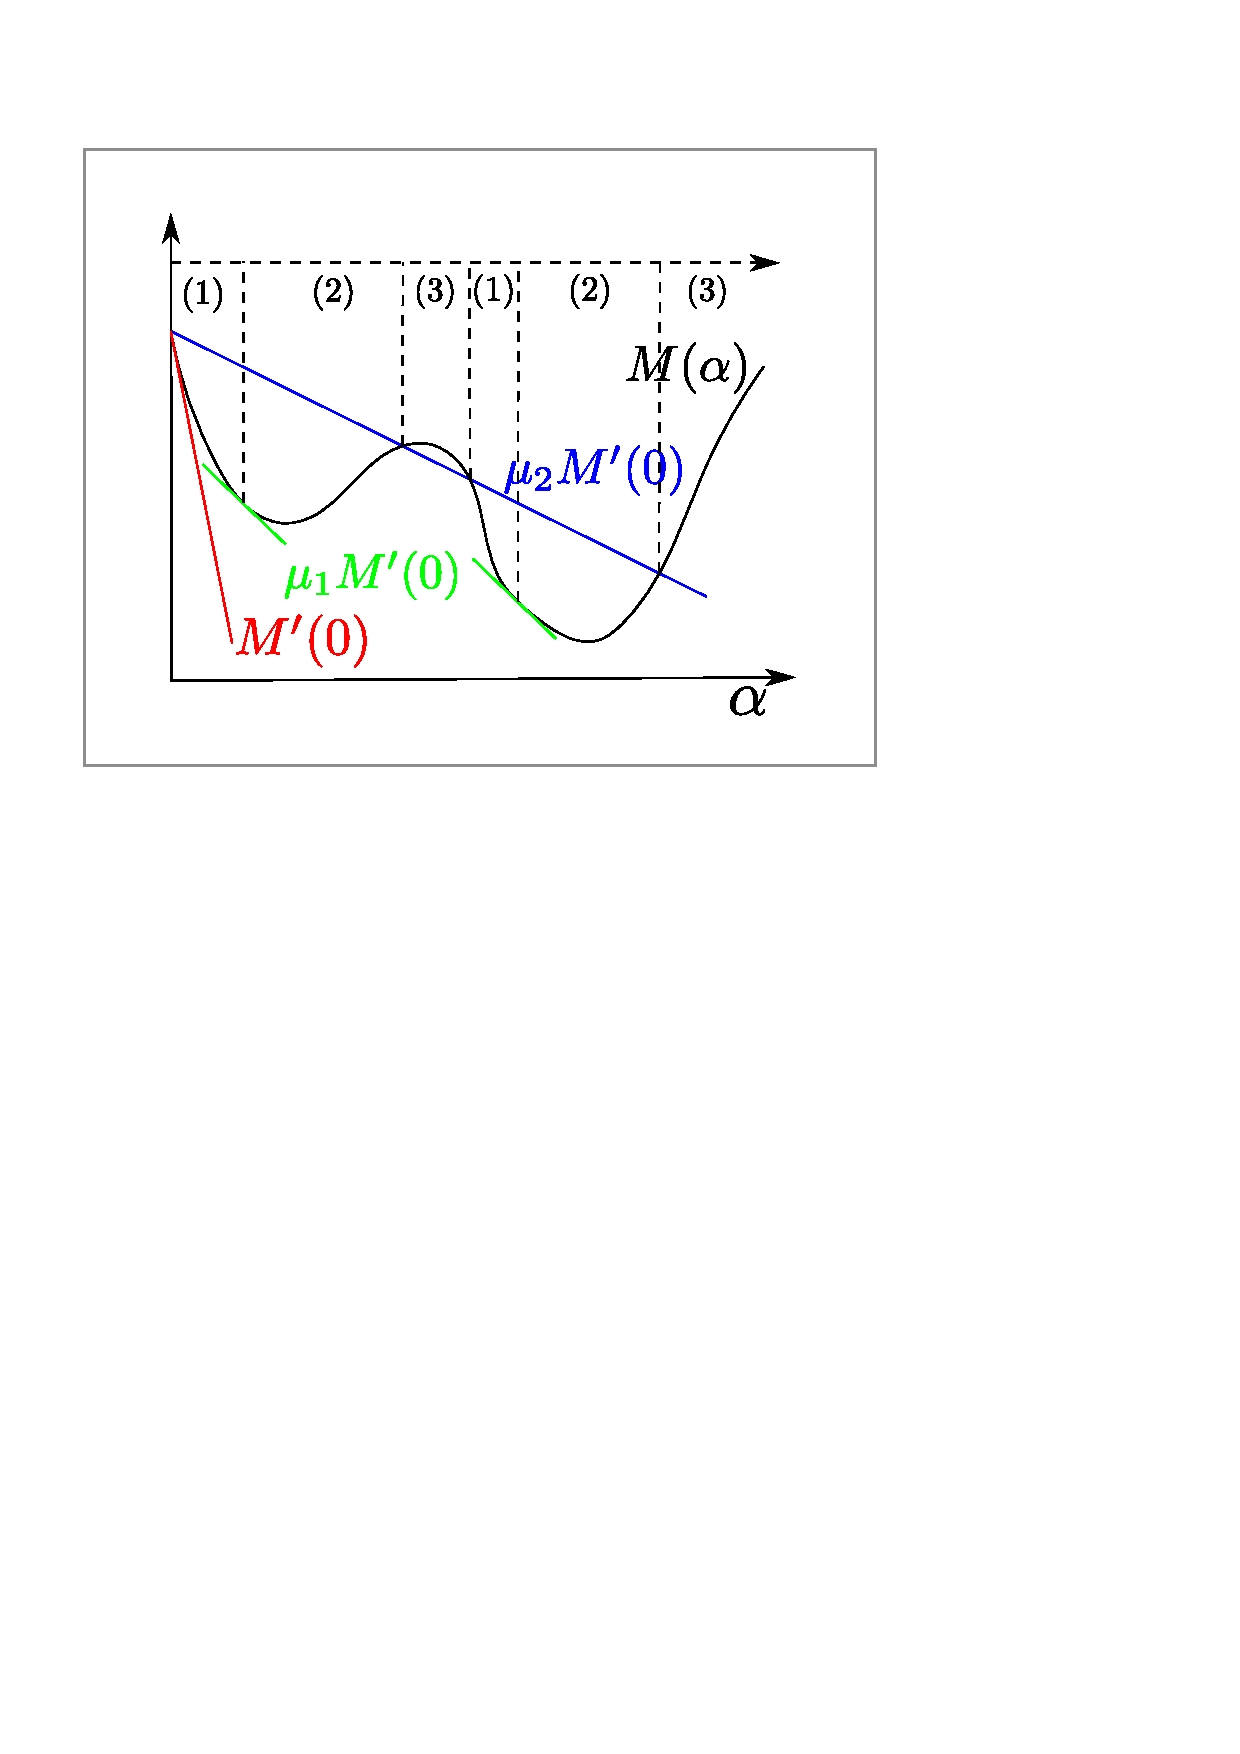
\includegraphics[width=0.7\textwidth]{line-search.pdf}
  \caption{Illustration of the choice made by the Wolfe line-search for values of $\alpha$}
\label{fig:Wolfe}
\end{figure}

The Wolfe line-search is popular, but it requires the computation of the derivative of the merit function, which can be prohibitively expensive in some cases, including in posture generation for robotics problems, where the derivatives are usually expensive.
Other line-search methods exist that do not require the derivative of $M$ for $\alpha\neq0$. For example the Goldstein and Price, or the Armijo methods.

\subsubsection{The filter method}
\label{ssub:the_filter_method}
The decision to accept on not a step generated by the QP can be made using a Filter approach instead of the Wolfe line search, as introduced by Fletcher in~\cite{fletcher:mathprog:2000}.
The goal of that method is to minimize the cost function $f(x)$ and the constraint violation $h(x)$ separately.
A step is accepted if it improves at least one of the function or the constraint violation.
\begin{equation}
  h(x) = \sum\limits_{k\in E} |c_k(x)| + \sum\limits_{k\in I} \max(0, -c_k(x))
\end{equation}

Denoting $h_i = h(x_i)$ and $f_i = f(x_i)$, we define the notion of domination as follows:
\begin{definition}
  \begin{equation}
    p_i\ \text{dominates }p_j \Leftrightarrow \left\{
        \begin{array}{l}
    f_i < f_j \\
    h_i < h_j
  \end{array}  \right.
  \end{equation}
\end{definition}

The filter maintains a list of pairs $p_i=\{f_i, h_i\}$ such that no pair dominates any other pair.
When a new point $x$ is submitted to the filter for acceptance, the values $f(x)$ and $h(x)$ are computed and the pair $p = \{f(x), h(x)\}$ is compared to every pair $p_i$.
If there is at least one pair $p_i$ in the filter that dominates $p$, the point is refused.
Otherwise, no pair of the filter dominates $p$, then $p$ is accepted and added to the filter.
Once $p$ is added to the filter, any pair in the filter that is dominated by $p$ is removed from it to ensure to keep a list of pairs non-dominated by each other in the filter.
In order to ensure global convergence, this method requires several refinements as explained in~\cite{fletcher:mathprog:2000}.
First, it needs to avoid accepting pairs that are excessively close to each other. For that, the domination criterion is modified with a sloping envelope, as proposed in Chin~\cite{chin:mathprog:2003}.
The sloping envelope definition takes user defined parameters $\beta$ and $\gamma$ in $[0,\ 1]$.

\begin{definition}
  \begin{equation}
    p_i\ \text{dominates }p_j \Leftrightarrow \left\{
        \begin{array}{l}
    f_i < f_j - \gamma h\ \\
    h_i < \beta h_j
  \end{array}  \right.
  \end{equation}
\end{definition}

\begin{figure}
  \centering
  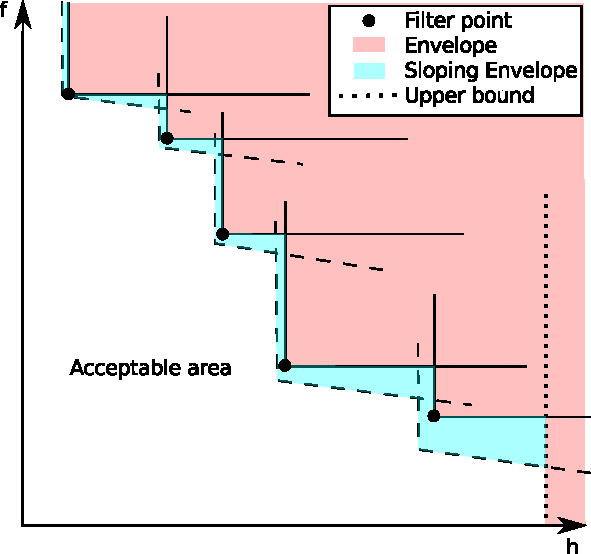
\includegraphics[width=0.7\textwidth]{filter.pdf}
  \caption{Representation of a filter with sloping envelope}
\label{fig:Filter}
\end{figure}

Another basic necessary improvement is to set an upper bound to the constraint violation, to avoid having the algorithm generate points that minimize the cost function while completely violating the constraints.

A representation of the filter method is given in figure~\ref{fig:Filter}

The filter method is convenient because it does not require the same complicated updates as can be found in penalty based methods where the penalty parameter needs to be updated regularly.
Also, with the filter method, no derivative computation is required.
That method is generally more permissive than merit-based method in the sense that it refuses fewer points.

The filter method, as well as the merit function based methods, can be used in line-search and trust-region algorithms.

\subsubsection{The Trust-Region Strategy}
\label{ssub:the_trust_region_strategy}
The Trust Region strategy is based on the idea that at any iterate $x_k$ the quadratic model made of the problem and fed to the QP solver can only be trusted to be relevant is a finite region around the iterate.
That region is called the trust region and its size is usually governed by a single positive parameter $\rho_k$ that can evolve along the optimization process.
This translates in a modified QP to solve at each iteration.
A boundary constraint describing the trust region is added to the problem.
At each step, the modified problem writes as:

\begin{equation}
  \begin{array}{ll}
    \minimize\limits_{z\in \mathbb{R}^n}{} & \frac{1}{2}z^T\nabla_{xx}^2Hz + \sum_{i\in\mathcal{U}}{\nabla c_i(x_k)}^T z \\
    \text{subject to } & {\nabla c_i(x_k)}^T z+c_i(x_k)=0,\ i\in \mathcal{F} \\
                       & {\nabla c_i(x_k)}^T z+c_i(x_k)\geq 0,\ i\in I\\
                       & |z|<\rho_k
  \end{array}
\label{approx_QP_TR}
\end{equation}

Once a solution $z$ of~\ref{approx_QP_TR} is found, the potential next iterate $x_{k+1} = x_k + z$ is checked against the acceptance criterion (should it be a merit function or a filter or other).
If it is accepted, that means that our current model is good, we move to the next step with $x_{k+1} \leftarrow x_k + z$, and the size of the trust region can be augmented based on some heuristics.
Otherwise, the iterate is refused, the model is less good than expected, the size of the trust region is reduced based on some heuristics (e.g. $\rho_{k+1}\leftarrow\rho_k /2$) and the problem~\ref{approx_QP_TR} is solved again with the new value of $\rho_{k+1}$.
This is repeated until a satisfying point is found, or until an infeasible problem is found.

\begin{figure}
  \centering
  \includegraphics[width=0.4\textwidth]{trust_region_incompatible.pdf}
  \caption{Constraint incompatibility generated by trust region approach}
\label{fig:TR_incompatible}
\end{figure}

With this approach, a problem that often arises is the generation of infeasible problems.
The reduction of the size of the trust region can lead to an incompatible set of constraints.
For example, with a single constraint, as illustrated in figure~\ref{fig:TR_incompatible}.
The linearisation of the constraint is represented by the green line, and the trust region by the black rectangle.
If $\rho$ is too small, there is no intersection between the linearization of the constraint and the trust region.
The QP is then infeasible.
An obvious solution for that would be to increase the size of the trust region, but that goes against the core idea of the trust region strategy and it would harm the convergence properties of the algorithm.
A more appropriate solution is to enter a restoration phase when that event occurs.
The purpose of a restoration phase is to reduce the infeasibility of a problem by relaxing infeasible constraints without regards for the cost function.
The restoration phase is exited once a feasible point is found, and the course of the SQP is continued from that point.

\subsection{Restoration phase}
\label{sub:restoration_phase}

As we stated previously, a restoration phase is entered when an infeasible problem is found by the trust region strategy.
The goal of the restoration is to find a solution to the following problem:

\begin{equation}
    \text{Find $x\in\mathbb{R}^n$ such that }
    \left\{
    \begin{array}{l}
      c_i(x)=0,\ i\in E \\
      c_i(x)\geq 0,\ i\in I\\
      |z|<\rho_k
    \end{array}
    \right.
\label{eq:resto_NL}
\end{equation}

The restoration phase proceeds in a similar way to the original SQP algorithm described earlier.
At each step, an approximated QP is solved, then its result is compared to an acceptance criterion, if it is accepted, the trust region can be increased and the algorithm continues.
Otherwise, the trust region is reduced and the problem is solved again.
The acceptance criterion must be tailored for the restoration problem, meaning that it is based on the values of the cost function of the restoration problem and of its constraints.
The big difference comes from the way the quadratic problem is constructed during this phase.

During a restoration phase step, the first action is to estimate the sets $\mathcal{F}$ and $\mathcal{I}$ of feasible  and infeasible constraints.
This is done by solving the linearization of problem~\Eqref{eq:resto_NL} as presented in~\Eqref{eq:FP}.
Each equality constraint is cut in 2 inequality constraints.

\begin{equation}
  \text{Find $z\in\mathbb{R}^n$ such that }
  \left\{
  \begin{array}{l}
    {\nabla c_i(x_k)}^T z+c_i(x_k)\geq 0,\ i\in E \\
    -{\nabla c_i(x_k)}^T z-c_i(x_k)\geq 0,\ i\in E \\
    {\nabla c_i(x_k)}^T z+c_i(x_k)\geq 0,\ i\in I\\
    |z|<\rho_k
  \end{array}
  \right.
\label{eq:FP}
\end{equation}

The resolution of that FP gives the lists $\mathcal{F}$ and $\mathcal{I}$.
If the list of infeasible constraints is empty, the problem is feasible, so the restoration phase is exited to return to the main SQP algorithm.
The restoration QP to solve is built based on those lists.
The infeasible constraints are removed from the constraint set and the expression of their violation is added to the cost function, while the feasible constraints remain in the constraint list.
This results in a problem like~\ref{rest_SQP} to solve.
(Note that the indexes of the constraints are modified to account for the duplication of the equality constraints)

\begin{equation}
  \begin{array}{ll}
    \minimize\limits_{z\in \mathbb{R}^n}{} & \frac{1}{2} z^T Hz - \sum\limits_{i\in\mathcal{I}}{\nabla c_i(x_k)}^T z \\
    \text{subject to } & {\nabla c_i(x_k)}^T z+c_i(x_k)\geq 0,\ i \in \mathcal{F} \\
                       & |z|<\rho_k
  \end{array}
\label{rest_SQP}
\end{equation}

This problem is solved by a QP solver, its result is checked against an acceptance criterion, based on that, the trust region is enlarged or reduced, and we go back to solving the FP\@.

In the restoration phase, special care must be taken in the computation of the matrix H, that represents the Hessian of the Lagrangian of a problem that changes at each iteration.
One possible approach is to compute it as the sum of the Hessians of all the individual constraints, and those can be computed exactly or with a quasi-newton approximation.


\subsection{Quasi-Newton Approximation}
\label{sub:quasi_newton_approximation}

In the SPQ algorithm, it is necessary to have access to the Hessian of the Lagrangian $\nabla_{xx}^2\mathcal{L}$ to be able to devise the QP subproblem to solve.
%For some strategies like the Line-Search, it is necessary that $\nabla_{xx}^2\mathcal{L}$ is definite positive.
Sometimes the exact Hessian of the problem is not positive definite.
Also, it is often difficult or computationally expensive to compute an exact Hessian of the Lagrangian.
Since we are following an iterative process, it is not necessary to have an exact knowledge of the Hessian and using an approximation of it is usually enough.
Also, an approximate Hessian is in most cases less expensive to compute than the exact one.

The idea behind computing an approximate Hessian is that, starting from an initial approximate Hessian $B_0$, we compute at each iteration an update to the approximate Hessian based on the values and first order derivatives of the Lagrangian.
This update aims at capturing some curvature information about the Hessian by evaluating the evolution of the gradient along the latest step.
At step $k$, the Hessian update is a function of $s_k$ and $y_k$:
\begin{equation}
  s_k = x_{k+1}-x_k,\ \ \ \
  y_k = \nabla_x\mathcal{L}(x_{k+1}, \lambda_{k+1}) - \nabla_x\mathcal{L}(x_{k}, \lambda_{k+1})
\end{equation}

The two most famous Hessian update strategies are called the BFGS (Broyden–Fletcher– Goldfarb–Shanno) and the SR1(Symmetric Rank 1) updates.
BFGS is a rank 2 update while SR1 is rank 1.

The most basic formulas for the BFGS update is the following:

\begin{equation}
\label{BFGS}
  B_{k+1} = B_k - \frac{B_k s_k s_k^T B_k}{s_k^T B_k s_k} + \frac{y_k y_k^T}{s_k^T y_k}
\end{equation}

Note that using a BFGS update requires that $s_k$ and $y_k$ satisfy the curvature condition: $s_k^T y_k>0$.
If that condition does not hold, then the value of $y_k$ is modified, which gives rise to the Damped BFGS update, which guarantees to keep $B_k$ definite positive:

\begin{equation}
\label{damped_BFGS}
\begin{split}
  \theta_k =
  \left\{
      \begin{array}{ll}
      1 & \text{if } s_k^T y_k \geq 0.2 s_k^T B_k s_k \\
      \frac{0.8 s_k^T B_k s_k}{s_k^T B_k s_k-s_k^T y_k} & \text{if } s_k^T y_k \geq 0.2s_k^T B_k s_k \\
      \end{array}
      \right.\\
      r_k = \theta_k y_k + (1-\theta_k) B_k s_k\\
      B_{k+1} = B_k-\frac{B_k s_k s_k^T B_k}{s_k^T B_k s_k} + \frac{r_k r_k^T}{s_k^T r_k}
\end{split}
\end{equation}

The SR1 update is computed with the following formula:

\begin{equation}
\label{SR1}
B_{k+1} = B_k + \frac{(y_k-B_k s_k){(y_k-B_k s_k)}^T}{{(y_k-B_k s_k)}^T s_k}
\end{equation}

Both those formulas proved to be efficient in some cases. It is not yet clear in which cases one is better than the other.

\section{Conclusion}
This section gives a general introduction to nonlinear constrained optimization without regards for specificities of robotics problem or formulations on manifolds, which are topics considered in the core of this thesis.


%
%%%%%%%%%%%%%%%%%%%%%%%%%%%%%%%%%%%%%%%%%%%%%%%%%%%%%%%%%%%%%%%%%%%%%%%
%                          Thesis Appendix B                          %
%                       Manifolds Descriptions                        %
%%%%%%%%%%%%%%%%%%%%%%%%%%%%%%%%%%%%%%%%%%%%%%%%%%%%%%%%%%%%%%%%%%%%%%%

\chapter{Manifolds Descriptions}
\label{appendix:manifolds}

\graphicspath{{Appendix2-Manifolds/Figs/}}

This appendix chapter comes as a complement for Chapter~\ref{chapter:optimization_on_noneuclidean_manifolds} in which we explicit the elements necessary for the description of several elementary manifolds.

%{{{ THE REAL SPACE MANIFOLD $\MATHBB{R^N$}
\section{The Real Space manifold}
\label{sec:the_real_space}
The Realspace manifold of dimension $n$ is denoted $\mathbb{R}^n$.
Since $\mathbb{R}^n$ is a Euclidean manifold, the operations that we use on it are straightforward.

\begin{table} [H]
\caption{Description of the $\mathbb{R}^n$ manifold}
\centering
\begin{tabular}{cc}
  \toprule
  $\mathcal{M}$ & $\mathbb{R}^n$ \\
  \midrule
  $\mathbb{E}$ & $\mathbb{R}^n$ \\
  \midrule
  $T_x\mathcal{M}$ & $\mathbb{R}^n$ \\
  \midrule
  $T_x\mathbb{E}$ & $\mathbb{R}^n$ \\
  \midrule
  $\phi_x(\mathbf{z})$ & $\mathbf{x} + \mathbf{z}$ \\
  \midrule
  $\partial \phi_x(0)$ & $\mathbb{I}_n$ \\
  \bottomrule
\end{tabular}
\quad
\begin{tabular}{cc}
  \toprule
  $\zeta(x,y)$ & $\mathbf{y} - \mathbf{x}$ \\
  \midrule
  $\frac{\partial \zeta_x}{\partial y}(x)$ & $\mathbb{I}_n$ \\
  \midrule
  $\mathcal{T}(x,\mathbf{z}, \mathbf{v})$ & $\mathbf{v}$ \\
  \midrule
  $\pi_\mathcal{M}(\mathbf{x})$ & $\mathbf{x}$ \\
  \midrule
  $\pi_{T_x\mathcal{M}}(\mathbf{z})$ & $\mathbf{z}$ \\
  \midrule
  $\lim$ & $\|\mathbf{v}\| \leq \infty$ \\
  \bottomrule
\end{tabular}
\end{table}
%}}}
%{{{ THE 3D ROTATION MANIFOLD SO(3): MATRIX REPRESENTATION
\section{The 3D Rotation manifold: Matrix representation}
\label{sec:the_3d_rotation_manifold_matrix_representation}

The 3D rotation manifold is denoted $SO(3)$.

An element $x$ of $SO(3)$ is represented by $\mathbf{x}=\psi(x)$ in $\mathbb{R}^{3\times 3}$ by:
\begin{equation}
  x\in SO(3),\ \mathbf{x} =\begin{bmatrix}
    x_{00} & x_{01} & x_{02} \\
    x_{10} & x_{11} & x_{12} \\
    x_{20} & x_{21} & x_{22} \\
  \end{bmatrix}
\end{equation}

We recall the operators
\begin{equation}
\widehat{.}: \begin{bmatrix}
  \omega_0\\\omega_1\\\omega_2\\
\end{bmatrix}
\rightarrow
\begin{bmatrix}
  0 & -\omega_2 & \omega_1 \\
  \omega_2 & 0 & -\omega_0 \\
  -\omega_1 & \omega_0 & 0\\
\end{bmatrix}
\end{equation}
And its inverse:
\begin{equation}
\widecheck{.}: \begin{bmatrix}
    x_{00} & x_{01} & x_{02} \\
    x_{10} & x_{11} & x_{12} \\
    x_{20} & x_{21} & x_{22} \\
\end{bmatrix}
\rightarrow
\begin{bmatrix}
  x_{21}\\x_{02}\\x_{10}\\
\end{bmatrix}
\end{equation}


The exponential map is known as the Rodrigues formula:
\begin{equation}
  \forall \mathbf{v}\in\mathbb{R}^3,\ \exp(\mathbf{v}) = \mathbb{I}_3 +
  \frac{\sin \|\mathbf{v}\|}{\|\mathbf{v}\|} \hat{\mathbf{v}} +
  \frac{1-\cos \|\mathbf{v}\|}{\|\mathbf{v}\|^2} \hat{\mathbf{v}}^2
\end{equation}

Note that when $\|\mathbf{v}\|$ is small, we make the following replacements to avoid numerical instability.
It is important to ensure the precision of the retractation near zero because in an optimization process, many small steps are taken, especially when close to the solution.

\begin{align}
 \frac{\sin \|\mathbf{v}\|}{\|\mathbf{v}\|} & = 1-\frac{\|\mathbf{v}\|}{6}\\
 \frac{1-\cos \|\mathbf{v}\|}{\|\mathbf{v}\|^2} & = 0.5 - \frac{\|\mathbf{v}\|}{24}
\end{align}

And the logarithm is computed as follows (see~\cite{merlhiot:thesis:2009}):
\begin{align}
\begin{split}
  \forall R\in\psi(SO(3)),\ f(R) &=
  \left\{ \begin{matrix}
  0 & \text{if }Tr(R) = 3 \\
  \frac{\arccos\left(\frac{Tr(R)-1}{2}\right)}{2\sin\left(\arccos\left(\frac{Tr(R)-1}{2}\right)\right)}\left(R-R^T\right) & \text{otherwise} \\
  \end{matrix} \right.\\
  \log(R) &= \widecheck{f\left(R\right)}
\end{split}
\end{align}

We consider a point $x\in\mathcal{M}$ and its representation matrix with the following storing order:
\begin{equation}
\mathbf{x}=\psi(x)
= \begin{pmatrix}
  x_0 & x_3 & x_6 \\
  x_1 & x_4 & x_7 \\
  x_2 & x_5 & x_8 \\
\end{pmatrix}
= \begin{pmatrix}
  x_{00} & x_{01} & x_{02} \\
  x_{10} & x_{11} & x_{12} \\
  x_{20} & x_{21} & x_{22} \\
\end{pmatrix}
\end{equation}

The derivative of retractation operation writes as:

\begin{align}
\label{eq:diffRetrSO3Matrix}
  \frac{\partial \varphi_x}{\partial \mathbf{z}}(0) =
  \begin{bmatrix}
    0 & -x_6 & x_3 \\
    0 & -x_7 & x_4 \\
    0 & -x_8 & x_5 \\
    x_6 & 0 & -x_0 \\
    x_7 & 0 & -x_1 \\
    x_8 & 0 & -x_2 \\
    -x_3 & x_0 & 0 \\
    -x_4 & x_1 & 0 \\
    -x_5 & x_2 & 0 \\
  \end{bmatrix}
\end{align}

And the derivation of the logarithm operation writes as:

\begin{align}
\label{eq:diffLogSO3Matrix}
  \mathbf{v} &= \begin{pmatrix}
    \frac{x_{21} - x_{12}}{2}\\
    \frac{x_{02} - x_{20}}{2}\\
    \frac{x_{10} - x_{01}}{2}\\
  \end{pmatrix} \\
  f &= \frac{\arccos \left( \frac{Tr(\mathbf{x})-1}{2} \right)}{2 \sin \left( \arccos \left( \frac{Tr(\mathbf{x})-1}{2} \right) \right) } \\
  df &= \frac{\left(Tr(\mathbf{x})-1\right)f-1}{2 \left( 1- {\left( \frac{Tr(\mathbf{x})-1}{2} \right)}^2 \right)} \\
  \frac{\partial \zeta_x}{\partial y}(x) &= \begin{bmatrix}
      & 0 & 0 & 0 &  & f & 0 & -f &  \\
    df.\mathbf{v} & 0 & -f & 0 & df.\mathbf{v} & 0 & f & 0 & df.\mathbf{v}  \\
      & f & 0 & -f &  & 0 & 0 & 0 &  \\
  \end{bmatrix}
\end{align}

\begin{table} [H]
\caption{Description of the $SO(3)$ manifold with matrix representation}
\centering
\begin{tabular}{cc}
  \toprule
  $\mathcal{M}$ & $SO(3)$ \\
  \midrule
  $\mathbb{E}$ & $\mathbb{R}^{3\times 3}$ \\
  \midrule
  $T_x\mathcal{M}$ & $\mathbb{R}^3$ \\
  \midrule
  $T_x\mathbb{E}$ & $\mathbb{R}^3$ \\
  \midrule
  $\psi(x) = \mathbf{x}$ & $ \begin{bmatrix}
    x_{00} & x_{01} & x_{02} \\
    x_{10} & x_{11} & x_{12} \\
    x_{20} & x_{21} & x_{22} \\
  \end{bmatrix} $ \\
  \midrule
  $\phi_x(\mathbf{z})$ & $\mathbf{x}\exp(\mathbf{z})$ \\
  \bottomrule
\end{tabular}
\quad
\begin{tabular}{cc}
  \toprule
  $\partial \phi_x(0)$ & see Equation~\ref{eq:diffRetrSO3Matrix} \\
  \midrule
  $\zeta(x,y)$ & $\log(\mathbf{x}^T\mathbf{y})$ \\
  \midrule
  $\frac{\partial \zeta_x}{\partial y}(x)$ & see Equation~\ref{eq:diffLogSO3Matrix} \\
  \midrule
  $\mathcal{T}(x,\mathbf{z}, \mathbf{v})$ & $\mathbf{v}$ \\
  \midrule
  $\pi_\mathcal{M}(\mathbf{x})$ & Q from QR decomposition of $\mathbf{x}$ \\
  \midrule
  $\pi_{T_x\mathcal{M}}(\mathbf{z})$ & $\mathbf{z}$ \\
  \midrule
  $\lim$ & $\|\mathbf{v}\| \leq \pi$ \\
  \bottomrule
\end{tabular}
\end{table}

%}}}

%{{{ THE 3D ROTATION MANIFOLD SO3 QUATERNION REPRESENTATION
\section{The 3D Rotation manifold with quaternion representation}
\label{sec:the_3d_rotation_manifold_quaternion_representation}

The 3D rotation manifold is denoted $SO(3)$.

An element $x$ of $SO(3)$ is represented by $\mathbf{q}=\psi(x)$ in $\mathbb{R}^{4}$ by:
\begin{equation}
  x\in SO(3),\ \mathbf{q} =\begin{bmatrix}
    q_{w}\\
    q_{x}\\
    q_{y}\\
    q_{z}\\
  \end{bmatrix}
  =\begin{bmatrix}
    q_{w}\\
    \mathbf{q_{vec}}\\
  \end{bmatrix}
\end{equation}

The exponential map is:
\begin{equation}
  \exp\ :\left|
  \begin{array}{ccc}
    \mathbb{R}^3 & \rightarrow & \mathbb{R}^4 \\
    \mathbf{z} & \mapsto & \begin{bmatrix}
      \cos \left( \frac{\|\mathbf{z}\|}{2} \right)\\
      \sin \left( \frac{\|\mathbf{z}\|}{2} \right) \frac{\mathbf{z}}{\|\mathbf{z}\|}\\
    \end{bmatrix} \\
  \end{array} \nonumber%
  \right.
\end{equation}

Note that when $\|\mathbf{v}\|$ is small, we make the following replacements to avoid numerical instability.

\begin{equation}
  \exp(\mathbf{z}) = \begin{bmatrix}
    1 -\frac{\|\mathbf{z}\|}{8} + \frac{{\|\mathbf{z}\|}^2}{384}\\
    \left(0.5 - \frac{\|\mathbf{z}\|}{48} + \frac{{\|\mathbf{z}\|}^2}{3840}\right)\mathbf{z}
  \end{bmatrix}
\end{equation}

And the logarithm is:
\begin{equation}
  \log\ :\left|
  \begin{array}{ccc}
    \mathbb{R}^4 & \rightarrow & \mathbb{R}^3 \\
    q & \mapsto & \arctan \left( \frac{2 \|\mathbf{q_{vec}}\| q_w}{q_w^2 - {\|\mathbf{q_{vec}\|}^2}} \right) \frac{\mathbf{q_{vec} } }{\|\mathbf{q_{vec}}\|} \\
  \end{array}
  \right.
\end{equation}

We consider a point $q\in\mathcal{M}$ and its representation quaternion with the following storing order:
\begin{equation}
\mathbf{q}=\psi(q)
= \begin{pmatrix}
  q_w \\
  q_x \\
  q_y \\
  q_z \\
\end{pmatrix}
\end{equation}

The derivative of retractation operation writes as:

\begin{align}
\label{eq:diffRetrSO3Quat}
  \frac{\partial \varphi_q}{\partial \mathbf{z}}(0) = \frac{1}{2}
  \begin{bmatrix}
    -q_x & -q_y & -q_z \\
     q_w & -q_z &  q_y \\
     q_z &  q_w & -q_x \\
    -q_y &  q_x &  q_w \\
  \end{bmatrix}
\end{align}

And the derivation of the logarithm operation writes as:

\begin{align}
\label{eq:diffLogSO3Quat}
  f &= \frac{\arctan \left( \frac{2 \|\mathbf{q_{vec}}\| q_w}{q_w^2 - {\|\mathbf{q_{vec}}\|}^2} \right)}{n}\\
  g &= \frac{2 q_w - f}{{\|\mathbf{q_{vec}}\|}^2} \\
  \frac{\partial \zeta_x}{\partial y}(\mathbf{x}) &= \begin{bmatrix}
  \begin{pmatrix}
    \\
    -2\mathbf{q_{vec}}\\
    \\
  \end{pmatrix} &
  \begin{pmatrix}
    \\
    f\mathbb{I}_3 + g\mathbf{q_{vec}}\mathbf{q_{vec}}^T\\
    \\
  \end{pmatrix}
  \end{bmatrix}
\end{align}


\begin{table} [H]
\caption{Description of the $\mathbf{SO(3)}$ manifold with quaternion representation}
\centering
\begin{tabular}{cc}
  \toprule
  $\mathcal{M}$ & $SO(3)$ \\
  \midrule
  $\mathbb{E}$ & $\mathbb{R}^{4}$ \\
  \midrule
  $T_x\mathcal{M}$ & $\mathbb{R}^3$ \\
  \midrule
  $T_x\mathbb{E}$ & $\mathbb{R}^3$ \\
  \midrule
  $\phi_x(\mathbf{z})$ & $\mathbf{x}\exp(\mathbf{z})$ \\
  \midrule
  $\partial \phi_x(0)$ & see Appendix~\ref{eq:diffRetrSO3Quat} \\
  \bottomrule
\end{tabular}
\quad
\begin{tabular}{cc}
  \toprule
  $\zeta(x,y)$ & $\log(\mathbf{x}^{-1}\mathbf{y})$ \\
  \midrule
  $\frac{\partial \zeta_x}{\partial y}(x)$ & see Appendix~\ref{eq:diffLogSO3Quat} \\
  \midrule
  $\mathcal{T}(x,\mathbf{z}, \mathbf{v})$ & $\mathbf{v}$ \\
  \midrule
  $\pi_\mathcal{M}(\mathbf{x})$ & $\frac{\mathbf{x}}{\|\mathbf{x}\|}$ \\
  \midrule
  $\pi_{T_x\mathcal{M}}(\mathbf{z})$ & $\mathbf{z}$ \\
  \midrule
  $\lim$ & $\|\mathbf{v}\| \leq \pi$ \\
  \bottomrule
\end{tabular}
\end{table}

%}}}


%{{{ THE UNIT SPHERE MANIFOLD $S2$
\section{The Unit Sphere manifold}
\label{sec:the_unit_sphere_manifold_s2}

An element $x$ of $S2$ is represented by $\mathbf{x}=\psi(x)$ in $\mathbb{R}^{3}$ by:
\begin{equation}
  x\in S2,\ \mathbf{x} =\begin{bmatrix}
    x_0\\
    x_1\\
    x_2\\
  \end{bmatrix}
\end{equation}

With this manifold, the tangent space at $x$ is the tangent plane to the unit-sphere at $x$.
Thus, $T_x\mathcal{M}$ it is a 2-dimensional space, and its representation space is $\mathbb{R}^3$.
%A tangent vector to $x$, $\mathbf{z}$, is such that $\mathbf{x}\cdot \mathbf{z} = \mathbf{x}^T\mathbf{z}=0$.

For the retractation we simply use a normalized sum:
\begin{equation}
  \phi_x(\mathbf{z}) = \frac{\mathbf{x}+\mathbf{z}}{\|\mathbf{x}+\mathbf{z}\|}
\end{equation}

We define a distance operation on $S2$ as:
\begin{equation}
  \dist(x, y) = 1-\mathbf{x}\cdot \mathbf{y}
\end{equation}

And the projection on the tangent space:
\begin{equation}
  \pi_{T_x\mathcal{M}}(\mathbf{z}) = \mathbf{z} - (\mathbf{x} \cdot \mathbf{z}) \mathbf{x}
\end{equation}

The pseudo-logarithm operation is the following:
\begin{equation}
  \zeta_x(y) = \dist(x,y)\frac{\pi_{T_x\mathcal{M}}(\mathbf{z})}{\|\pi_{T_x\mathcal{M}}(\mathbf{z})\|}
\end{equation}

The vector transport operation of vector $\mathbf{v}$ from $T_x\mathcal{M}$ to $T_y\mathcal{M}$ with $y = \phi_x(\mathbf{v})$, corresponds to rotating $\mathbf{v}$ by the rotation that transforms $x$ into $y$:
\begin{align}
  &\mathbf{y} = \phi_x(\mathbf{z}) \\
  &R = \mathbb{I}_3 + \widehat{\mathbf{x} \wedge \mathbf{y}} + \frac{{\widehat{\mathbf{x} \wedge \mathbf{y} } }^2}{1+\mathbf{x}\cdot\mathbf{y}} \\
  &\mathcal{T}(x,\mathbf{z}, \mathbf{v}) = R\mathbf{v}
\end{align}

\begin{table} [H]
\caption{Description of the S2 manifold}
\centering
\begin{tabular}{cc}
  \toprule
  $\mathcal{M}$ & $S2$ \\
  \midrule
  $\mathbb{E}$ & $\mathbb{R}^{3}$ \\
  \midrule
  $T_x\mathcal{M}$ & $\mathbb{R}^2$ \\
  \midrule
  $T_x\mathbb{E}$ & $\mathbb{R}^3$ \\
  \midrule
  $\phi_x(\mathbf{z})$ & $\frac{\mathbf{x}+\mathbf{z}}{\|\mathbf{x}+\mathbf{z}\|}$ \\
  \midrule
  $\partial \phi_x(0)$ & $\mathbb{I}_3 - \mathbf{x}\cdot\mathbf{x}^T$ \\
  \bottomrule
\end{tabular}
\quad
\begin{tabular}{cc}
  \toprule
  $\zeta(x,y)$ & $\mathbf{y} - (\mathbf{x} \cdot \mathbf{y}) \mathbf{x}$ \\
  \midrule
  $\frac{\partial \zeta_x(x)}{\partial y}$ & $\mathbb{I}_3 -\mathbf{x}\cdot\mathbf{x}^T$ \\
  \midrule
  $\mathcal{T}(x,\mathbf{z}, \mathbf{v})$ & $\mathbb{I}_3 + \widehat{\mathbf{x} \wedge \phi_x(\mathbf{z})} + \frac{{\widehat{\mathbf{x} \wedge \phi_x(\mathbf{z})}}^2}{1+\mathbf{x}\cdot\phi_x(\mathbf{z})}$ \\
  \midrule
  $\pi_\mathcal{M}(\mathbf{x})$ & $\frac{\mathbf{x}}{\|\mathbf{x}\|}$ \\
  \midrule
  $\pi_{T_x\mathcal{M}}(\mathbf{z})$ & $\mathbf{z} - (\mathbf{x} \cdot \mathbf{z}) \mathbf{x}$ \\
  \midrule
  $\lim$ & $\|\mathbf{v}\| \leq \infty$ \\
  \bottomrule
\end{tabular}
\end{table}

%}}}


\end{appendices}

% *************************************** Index ********************************
\printthesisindex % If index is present

\end{document}
